%% LyX 2.3.7 created this file.  For more info, see http://www.lyx.org/.
%% Do not edit unless you really know what you are doing.
\documentclass[11pt,thmsb]{article}
\usepackage[latin9]{inputenc}
\usepackage{geometry}
\geometry{verbose,tmargin=1in,bmargin=1in,lmargin=1in,rmargin=1in,headheight=1cm,headsep=1cm,footskip=1cm}
\synctex=-1
\usepackage{color}
\usepackage{array}
\usepackage{verbatim}
\usepackage{float}
\usepackage{units}
\usepackage{textcomp}
\usepackage{amsmath}
\usepackage{amsthm}
\usepackage{amssymb}
\usepackage{graphicx}
\usepackage[authoryear]{natbib}

\makeatletter

%%%%%%%%%%%%%%%%%%%%%%%%%%%%%% LyX specific LaTeX commands.
%% Because html converters don't know tabularnewline
\providecommand{\tabularnewline}{\\}

%%%%%%%%%%%%%%%%%%%%%%%%%%%%%% Textclass specific LaTeX commands.
\theoremstyle{plain}
\newtheorem{lem}{\protect\lemmaname}
\theoremstyle{plain}
\newtheorem{thm}{\protect\theoremname}
\theoremstyle{plain}
\newtheorem{cor}{\protect\corollaryname}
\theoremstyle{definition}
\newtheorem{defn}{\protect\definitionname}
\theoremstyle{plain}
\newtheorem{prop}{\protect\propositionname}

%%%%%%%%%%%%%%%%%%%%%%%%%%%%%% User specified LaTeX commands.
%2multibyte Version: 5.50.0.2960 CodePage: 1251
%              Scientific Word   Wrap/Unwrap  Version 2.5             %
%              Scientific Word   Wrap/Unwrap  Version 3.0             %
% If you are separating the files in this message by hand, you will   %
% need to identify the file type and place it in the appropriate      %
% directory.  The possible types are: Document, DocAssoc, Other,      %
% Macro, Style, Graphic, PastedPict, and PlotPict. Extract files      %
% tagged as Document, DocAssoc, or Other into your TeX source file    %
% directory.  Macro files go into your TeX macros directory. Style    %
% files are used by Scientific Word and do not need to be extracted.  %
% Graphic, PastedPict, and PlotPict files should be placed in a       %
% graphics directory.                                                 %
% Graphic files need to be converted from the text format (this is    %
% done for e-mail compatability) to the original 8-bit binary format. %
% Files included:                                                     %
% "/document/NonbalancedJune18.tex", Document, 124302, 6/18/2004, 0:45:10, ""%
% "/document/HZH9JA00.wmf", PastePict, 30602, 6/17/2004, 21:53:40, "" %
% "/document/HZH9JA01.wmf", PastePict, 31310, 6/17/2004, 21:55:05, "" %
% "/document/HZH9JA02.wmf", PastePict, 31498, 6/17/2004, 21:56:09, "" %
% "/document/HXIWF402.wmf", ImportPict, 31112, 6/11/2004, 2:52:58, "" %
% "/document/figure1new.wmf", ImportPict, 8034, 6/11/2004, 2:52:58, ""%
% "/document/HZH9JA03.wmf", PastePict, 49212, 6/11/2004, 2:52:58, ""  %
%%%%%%%%%%%%%%%% Start /document/NonbalancedJune18.tex %%%%%%%%%%%%%%%%


%%%%%%%%%%%%%%%%%%%%%%%%%%%%%%%%%%%%%%%%%%%%%%%%%%%%%%%%%%%%%%%%%%%%%%%%%%%%%%%%%%%%%%%%%%%%%%%%%%%%%%%%%%%%%%%%%%%%%%%%%%%%%%%%%%%%%%%%%%%%%%%%%%%%%%%%%%%%%%%%%%%%%%%%%%%%%%%%%%%%%%%%%%%%%%%%%%%%%%%%%%%%%%%%%%%%%%%%%%%%%%%%%%%%%%%%%%%%%%%%%%%%%%%%%%%%
\usepackage{amsfonts}
\usepackage{version}
\usepackage[font=footnotesize,singlelinecheck=true,format=plain,justification=RaggedRight]{caption}



\setcounter{MaxMatrixCols}{10}
%TCIDATA{TCIstyle=article/art4.lat,lart,article}

%TCIDATA{OutputFilter=LATEX.DLL}
%TCIDATA{Version=5.50.0.2960}
%TCIDATA{Codepage=1251}
%TCIDATA{<META NAME="SaveForMode" CassONTENT="1">}
%TCIDATA{BibliographyScheme=BibTeX}
%TCIDATA{Created=Sat Jul 31 12:49:26 1999}
%TCIDATA{LastRevised=Thursday, July 08, 2021 13:53:15}
%TCIDATA{<META NAME="GraphicsSave" CONTENT="32">}
%TCIDATA{Language=American English}
%TCIDATA{CSTFile=LaTeX article (bright).cst}

\input{tcilatex}
\textwidth 6.2in \textheight 8.65in \setlength{\topmargin}{-0.4in}
\setlength{\oddsidemargin}{0.15in}
\setlength{\evensidemargin}{0.15in}
\usepackage{url}

\usepackage{tikz}
\usepackage{pgfplots}
\usepackage{pgfplotstable}
\pgfplotsset{compat=newest}
\usepgfplotslibrary{dateplot}
\usepgfplotslibrary{groupplots}
\usepgfplotslibrary{fillbetween}
\usepgfplotslibrary{dateplot}

\providecommand{\corollaryname}{Corollary}
\providecommand{\definitionname}{Definition}
\providecommand{\lemmaname}{Lemma}
\providecommand{\propositionname}{Proposition}
\providecommand{\theoremname}{Theorem}



\newcommand{\TS}[1]{{\textcolor{red}{#1}}}
\newcommand{\LPH}[1]{{\textcolor{blue}{#1}}}

\@ifundefined{showcaptionsetup}{}{%
 \PassOptionsToPackage{caption=false}{subfig}}
\usepackage{subfig}
\makeatother

\providecommand{\corollaryname}{Corollary}
\providecommand{\definitionname}{Definition}
\providecommand{\lemmaname}{Lemma}
\providecommand{\propositionname}{Proposition}
\providecommand{\theoremname}{Theorem}


%\usepackage{tikz}
%\usetikzlibrary{external}
%\tikzexternalize % Activate externalization
%\tikzsetexternalprefix{figdata/} % Directory for externalized files
\usepackage{xr} % Enable external references
\externaldocument{final_submission_jpe_webappx}


\begin{document}
\author{L\'{e}o Aparisi de Lannoy \\
 %EndAName
University of Chicago \and Anmol Bhandari \\
 %EndAName
University of Minnesota \and David Evans \\
 %EndAName
University of Oregon \and Mikhail Golosov \\
 %EndAName
University of Chicago \and Thomas Sargent \\
 %EndAName
NYU}
\title{\textbf{Managing Public Portfolios}\thanks{We thank Marios Angeletos, Deborah Lucas, Hanno Lustig, and Benjamin
Moll for discussions earlier drafts along with audiences at Chicago,
Penn State, TSU, UPenn, UCLA, Bank of Portugal, NBER Asset Pricing
Meeting, Bank of Finland, Bank of Italy, Penn State, Arizona State
University, Carnegie Mellon University, College de France, MIT, St.
Louis Fed, Minneapolis Fed, Wharton, Wisconsin, Yale, IMF, and the
University of Padua. We thank Jiawei Fan and Judy Yue for excellent
research assistance. Bhandari, Evans, and Golosov thank the NSF\
for support (grant \#36354.00.00.00).}}
\date{October 2024\bigskip{}
}

\maketitle
\bigskip{}
 \bigskip{}

\begin{center}
\textbf{Abstract}
\par\end{center}

We study optimal public portfolios in a class of macro-finance models
that includes widely-used specifications of households' risk and liquidity
preferences, market structures for financial assets, and trading frictions.
An optimal portfolio hedges fluctuations in interest rates, primary
surpluses, and income inequalities. We express an optimal portfolio
in terms of statistics that are functions only of macro and financial
market data. An application to U.S. data shows that hedging interest
rate risk plays a dominant role in shaping an optimal maturity structure
of U.S. government debt.

\newpage{}

\setcounter{page}{1}

\baselineskip0.64cm

\section{Introduction}

\vspace{0in}

We characterize main forces that shape optimal public portfolios of
financial assets in a large class of stochastic economies in which
a government uses distortionary taxes to raise revenues and finance
expenditures. We provide formulas for optimal portfolios in terms
of a small number of statistics that are functions of observables.
For U.S. data, an optimal portfolio's bond shares decrease approximately
exponentially with increases in their maturity. % and that its maturity structure, though similar to the
%U.S., has a longer duration.

We begin by studying an environment that shares many features with
the Ramsey literature on optimal taxation and debt management. We
consider an economy with a representative, infinitely lived household
that derives utility from consumption and leisure. We abstract from
income effects on labor supplies but allow various attitudes about
risk, model ambiguity, and intertemporal substitution. A benevolent
government uses distortionary taxes to finance exogenous public expenditures.
Households and the government trade an exogenous set of financial
assets. %The set of financial assets is
%exogenous but arbitrary. 
Our benchmark model is a small open economy in which large foreign
investors trade these financial and assets determine their prices.

We develop a new approach to study optimal government policies that
builds on two key ideas. The first idea, inspired by the ``sufficient
statistics'' approach in public finance, is to study consequences
of perturbing government policies along histories of a competitive
equilibrium allocation. Welfare impacts of such policies can be isolated
using the envelope theorem. The second idea is to use ``small noise''
expansions to simplify formulas, making them analytically tractable
and convenient for empirical applications. By combining these two
ideas, we derive explicit formulas that characterize an optimal public
portfolio in terms of population moments with sample counterparts
in macro and financial market data.

In our benchmark economy, fluctuations in government spending directly
affect primary surpluses. Fluctuations in future interest rates make
costs of rolling over debt obligations uncertain. Costs of distortionary
taxation motivate the government to structure its portfolio to make
the return on the portfolio offset these fluctuations, thereby attenuating
variations in tax rates. Our formulas express an optimal government
portfolio as a sum of two terms. One captures hedging of fluctuations
in primary surpluses. Another captures hedging of fluctuations in
risk-free interest rates on zero coupon bonds of various maturities.
These terms depend on determinants with empirical counterparts, such
as covariances of excess returns of each security with excess returns
of other securities, government expenditures, and interest rates on
bonds of various maturities. We also show that, up to orders of approximation
under consideration here, these variables are independent of a government's
portfolio choices, so that even if actual portfolio choices are suboptimal,
we can construct these statistics from the data and plug them into
our formula for optimal public portfolios.

Our formulas bring significant insights. First, our formula for an
optimal portfolio includes no terms that summarize risk premia or
risk aversion, thereby indicating a key difference between classical
portfolio theory for private investors (e.g., Samuelson (1970), Merton
(1971)) and our prescriptions for public portfolios. This difference
casts doubt on the practice of many treasury departments and finance
ministries of exploiting differences in borrowing costs across bonds
of different maturities to reduce debt financing costs. Our model
asserts that this practice is suboptimal because households can exploit
those differences themselves without bearing deadweight losses from
taxation.

Although our formulas apply to all securities that a government can
trade, they offer specific additional insights when those securities
are bonds of various maturities. The return on a bond of maturity
$k$ co-moves mechanically with a $k$-period interest rate, implying
that the government can use bonds to hedge interest rate risk perfectly.
Such a portfolio embodies a simple ``maturity-matching'' principle
that prescribes that the quantity of bonds of maturity $k$ should
be proportional to expected primary surpluses $k$ periods ahead.%
\begin{comment}
When converted to portfolio shares, this principle implies that optimal
bond portfolio share of maturity $k$ is equal to the price of the
bond of that duration times the expected growth in primary surpluses
in the next $k$ periods. We refer to this portfolio as the growth-adjusted
price curve. The departures of the optimal portfolio, that hedges
all risks, from the growth-adjusted price curve is driven by how closely
excess returns of bonds of different maturities co-move with fluctuations
in government expenditures.
\end{comment}

We apply our approach to determinants of optimal public portfolios.
We examine roles of uncertainty about tax revenues, additional liquidity
services that government bonds may provide, and household heterogeneities
that include inabilities of some households to participate in asset
markets. %Our method of combining policy perturbations with small noise expansions
%remains tractable in these complicated environments. I
%In all cases,
We derive statistics that express influences of these determinants
and that can be estimated from data. We also move beyond a small open
economy and consider several models of asset price determination,
including preferred habitat models. Our analysis shows that when the
government faces downward-sloping demand curves for its debt, it tilts
its portfolio to avoid circumstances that call for large rebalancings.

We apply our framework to prescribe an optimal composition of U.S.
debt. We use data on returns of U.S. government, taxes, and primary
surpluses to construct each component of an optimal portfolio. As
a starting point, we restrict our attention to bonds with up to 30
years maturity. We find debt portfolio shares decline approximately
geometrically with maturity. The optimal portfolio has a shape qualitatively
similar to the actual U.S. portfolio but with longer duration.

Interest rate risk contributes most to the shape of the optimal portfolio.
Empirically, covariances of bond returns with government expenditures
and revenues are small, implying small scope for using these bonds
to hedge such risks. Scope of trading bonds to hedge other risks,
such as inequality risks, also appears to be small. If the demand
for U.S. bonds were perfectly elastic, an optimal portfolio of bonds
would be very similar to one that adheres to the maturity matching
principle. This portfolio would have a duration of about 9.6 years;
much longer than the duration of the U.S. debt which is about 5 years.
Such a portfolio, however, requires substantial reissuances of 30-year
bonds each year, which is costly when demand for those bonds is downward
sloping. Using demand elasticities gathered from the literature, the
optimal portfolio tilts toward shorter maturities but not as much
the U.S. portfolio. 

Our analysis suggests that issuing bonds with maturities beyond 30
years has several benefits. First, it improves hedging of interest
rate risk over longer time horizons. Second, it reduces the fraction
of debt that needs to be reissued each period, mitigating adverse
price impact. We find that the portfolio of bonds with maturities
up to 50 years is very close to the one obtained under the maturity
matching principle.% Our analysis indicates that the portfolio of bonds with
%maturities up to 50 years is very close to the one obtained under
%the maturity matching principle.

In the final part of the paper, we study connections between our findings
and the widely-cited results in the Ramsey literature on optimal debt
management. A striking finding in that literature highlighted by \citet{BueraNicolini_etalJME2004}
is that the optimal portfolio of bonds in a calibrated neoclassical
model is extreme: holdings of bonds with specific maturities can equal
hundreds or thousands times annual GDP, and portfolio shares of bonds
with similar maturities often take opposite signs. Using a calibrated
economy similar to \citeauthor{BueraNicolini_etalJME2004}'s (2004),
we construct two portfolios: the exact optimal bond portfolio prescribed
by formulas of \citet{AngeletosQJE2002}, and the approximate portfolio
implied by our formulas.  The two portfolios are very similar and have the peculiar large  long-short positions  noted by \citet{BueraNicolini_etalJME2004}.
We use our formulas to investigate sources of that portfolio structure. We find
that simulated data from the calibrated economy have variances of
bond excess returns that are substantially lower, correlations of
bond returns with macroeconomic variables that are substantially higher,
and often of different signs than their empirical counterparts. We
show that augmenting this model with discount factor shocks can bring
these statistics closer to their empirical counterparts, at which
point the optimal portfolio becomes similar to the one we constructed
via our sufficient statistics for U.S. data.

\vspace{0in}


\paragraph*{Related Literature}

Our paper is related to an extensive Ramsey literature on the optimal
composition of government debt, such as \citet{LucasStokeyJME1983},
\citet{BohnAER1990}, \citet{zhu1992optimal}, \citet{Chari_etalJPE1994},
\citet{AngeletosQJE2002}, \citet{BueraNicolini_etalJME2004}, \citet{FarhiJPE2010},
\citet{Faraglia_etalReStud2018}, \citet{Lustig_etalJME2008}, \citet{Bhandari_etalQJE2017}.
Those authors used closed economy neoclassical growth models to characterize
optimal public portfolios. However, those models don't fit empirical
relationships among asset prices, asset supplies, and macroeconomic
variables, key objects that determine how well alternative securities
hedge risks. We overcome that deficiency by assuming more general
specifications of preferences and asset demands that includes \textit{\emph{multiple}}
forces that can account for the observed asset pricing behavior.

\begin{comment}
Realistic asset pricing dynamics dramatically change many insights
about optimal public portfolios that emerged from that earlier literature.
For example, in their quantitative model calibrated to the U.S. economy,
\citet{BueraNicolini_etalJME2004} find that the government should
issue long-term debt valued at tens or hundreds times GDP while simultaneously
taking offsetting short (i.e., negative) positions in short-term debt
of similar magnitudes. They also find that government holdings of
debts of similar maturities may differ by hundreds percent of GDP;
that the composition of the optimal portfolio is very sensitive to
the menu of traded maturities; and that relatively small aggregate
shocks caused very significant portfolio rebalancing. In contrast,
our optimal portfolio is very stable over time and has simple declining
maturity weights qualitatively like those observed in US data. We
show that the dramatic differences in these findings are driven by
counterfactual asset pricing implications of the standard neoclassical
growth model.
\end{comment}

Our paper builds on a literature in finance that focuses on asset
price determination, such as \citet{AiBansalECMA2018}, \citet{BansalYaronJF2004},
\citet{Albuquerque_etalJF2016}, \citet{KrishnamurthyVissingJorgensenJPE2012},
\citet{GreenwoodVayanosRFS2014}. Those authors modified the standard
neoclassical environment in ways designed to make it do a better job
of fitting asset prices. By setting up a framework broad enough to
include all of these structures and by deriving obtaining expressions
for optimal portfolios that depend on only a small number of statistics
that are functions of aggregates and asset returns, we sidestep taking
a stand on details of those structures.

We obtain formulas for optimal government portfolio that are related
to the formulas for private portfolios that appear in classic portfolio
theory contributions of \citet{SamuelsonReStud1970}, \citet{MertonReStat1969,MertonJET1971},
\citet{CampbellViceiraQJE1999,CampbellViceiraAER2001}, and \citet{ViceiraJF2001}.
Although individual investors in that theory and the government in
our model both choose portfolios to hedge their risks, we show that
substantially different forces determine portfolio compositions in
the two settings.

Our findings are also related to some recent work by \citet{Debortoli_etalQJE2017,Debortoli_etalAERI2022}.
For a deterministic version of \citet{LucasStokeyJME1983}, they find
that issuing a consol aligns incentives across successive governments
and eliminates time inconsistency. We study a timing protocol in which
government commits to a plan but nevertheless find that in a stationary
world the optimal portfolio is well approximated by a (growth-adjusted)
consol---a security that implements the maturity matching principle
and eliminates needs to rollover or rebalance the portfolio.\footnote{Our work is also related to \citet{Bigio_etalJPEM2023} who study
the optimal composition of government portfolios of bonds of different
maturities. They mostly abstract from the interest rate risk and primary
surplus risk that we emphasize, and focus on understanding how price
impacts from debt issuance affect portfolio composition. Because they
impose an exogenous cap on the maturities, the government in their
setup wants to rebalance its portfolio even in the absence of all
risks.}

In recent papers, \citet{Jiang_etalWP2019,Jiang_etalWP2020} document
a number of puzzling facts about market values of total debt and primary
surpluses in the U.S. These facts are puzzling when debt valuation
is viewed through the lens of an arbitrage-free and frictionless asset
pricing framework. Our setting departs from such a framework by incorporating
market segmentation as well as a broad notion of liquidity services
that U.S debts provide. However, in this paper we focus on how the
market value of government debt is optimally allocated across various
securities, and not on determinants of the level itself.

Methodologically, this paper relates to two strands of literature.
We borrow our approach of using a small number of statistics to characterize
an optimal government portfolio from a recent applied public finance
literature, notably \citet{SaezRestud2001} and \citet{ChettyAR2009}.
That literature typically focuses on settings in which a government
faces no risk. When applied to our problem, that approach yields no
clear and transparent insights. We make progress by deploying small-noise
approximations. Small noise approximations have been used frequently
both in finance (e.g., \citet{SamuelsonReStud1970}, \citet{DevereuxSutherlandJEEA2011})
and computational economics (e.g., \citet{GuuJuddET2001}, \citet{SchmittUribeJET2004},
\citet{BEGS2}). The particular class of expansions that we use does
not require us to assume stationarity or to ignore heteroskedasticity.
That makes it particularly suitable to study portfolio problems in
dynamic stochastic economies.

\paragraph*{Outline}

The rest of the paper is organized as follows. To demonstrate our
approach and convey main ideas, Sections \ref{sec: environment} and
\ref{sec: characerization benchmark} start with our simplest setting
(``benchmark economy''). In Section \ref{sec:Extensions}, we consider
several extensions of the benchmark economy. In Section \ref{sec: target portfolio},
we apply our theory to infer an optimal portfolio for the U.S. and
compare it to the observed portfolio. In Section \ref{sec: Comparing to neoclassical},
we contrast our findings to neoclassical settings studied in \citet{AngeletosQJE2002}
and \citet{BueraNicolini_etalJME2004}. Section \ref{sec:Conclusion}
concludes. Proofs of all statements in the main text are in the online
appendix.

\vspace{0in}


\section{A benchmark economy\label{sec: environment}}

We consider a discrete time infinite horizon economy. Uncertainty
is described by a stochastic process $\{s_{t}\}_{t}$, where $s_{t}\subset\mathbb{R}^{N}$
for some $N\leq\infty$. We use $s^{t}$ to denote the history of
shocks $\left(s_{0},....,s_{t}\right)$ and $s^{t+k}\succeq s^{t}$
to denote histories $s^{t+k}$ in which first $t+1$ elements are
equal to $s^{t}$. $\Pr\left(s^{t+k}\right)$ and $\Pr\left(s^{t+k}|s^{t}\right)$
denote probabilities of $s^{t+k}$ conditional on information in periods
0 and $s^{t}$, respectively.

We use $z_{t}$ to denote the vector of all exogenous shocks that
affect agents. These shocks are functions of $s_{t}$, i.e., $z_{t}=z_{t}\left(s_{t}\right)$,
so the stochastic process for $s_{t}$ determines $z_{t}$. For technical
reasons, we assume that $z_{t}$ is bounded. The conditional expectation
in history $s^{t}$ is denoted by $\mathbb{E}_{s^{t}}$, or $\mathbb{E}_{t}$
if the specific history $s^{t}$ is clear from the context.

The economy is inhabited by three groups of agents: households, the
government, and foreign investors. All agents trade a given set of
securities. A security $i$ is characterized by an exogenous stochastic
stream of dividends $\{D_{t}^{i}\}_{t}$. We use $Q_{t}^{i}$ to denote
the price of security $i$ and $R_{t+1}^{i}=(Q_{t+1}^{i}+D_{t+1}^{i})/Q_{t}^{i}$
to denote its holding period return from $t$ to $t+1$. A risk-free
bond is a security that pays one unit of dividend next period. Let
$Q_{t}^{rf}$ be the price of a risk-free bond and $R_{t+1}^{rf}=1/Q_{t}^{rf}$
be the risk-free interest. The excess return of security $i$ is $r_{t+1}^{i}=R_{t+1}^{i}-R_{t+1}^{rf}$.

In the benchmark economy, there is measure one of identical, infinitely-lived
households who supply effort to earn income $Y_{t}$, pay proportional
taxes $\tau_{t}$, and allocate after-tax income between consumption
$C_{t}$ and investing into a portfolio of securities. We use $\left\{ b_{t}^{i}\right\} _{i}$
to denote date $t$ market values of household investments. The household's
problem is 
\begin{equation}
V=\max_{\{C_{t},Y_{t},\{b_{t}^{i}\}_{i}\}_{t}}\mathbb{E}_{0}\sum_{t}\beta^{t}u\left(C_{t}-v\left(Y_{t}\right)\right)\label{eq: preferences HH}
\end{equation}
where maximization is subject to 
\begin{equation}
C_{t+1}+\sum_{i}b_{t+1}^{i}=\left(1-\tau_{t+1}\right)Y_{t+1}+\sum_{i}R_{t+1}^{i}b_{t}^{i},\label{eq: budget constraint HH}
\end{equation}
 given an initial portfolio $\{b_{-1}^{i}\}_{i}$ and natural borrowing
limits. Here $\beta$ is a discount factor, functions $u$ and $v$
are strictly increasing, twice differentiable, and $u$ and $-v$
are strictly concave.

The government sets tax rates $\left\{ \tau_{t}\right\} _{t}$ and
trades portfolios of securities to finance exogenous stochastic expenditures
$\{G_{t}\}_{t}.$ We use $T_{t}=\tau_{t}Y_{t}$ to denote tax revenues.
For all dates $t\geq-1$, the period-by-period government budget constraint
is 
\[
T_{t+1}-G_{t+1}+\sum_{i}B_{t+1}^{i}=\sum_{i}R_{t+1}^{i}B_{t}^{i},
\]
where a positive value of $B_{t}^{i}$ indicates the market value
of government's liability in security $i$. We adopt this sign convention
so that positive values indicate values of outstanding liabilities.

Government budget constraints play an important roles in our analysis
of optimal public portfolios. It will be helpful to re-write using
portfolio shares. Let $B_{t}:=\sum_{i}B_{t}^{i}$ be the total market
value of the government portfolio and $\omega_{t}^{i}=B_{t}^{i}/B_{t}$
be the portfolio share of security $i$. We refer to $B_{t}$ as the
government's debt level, and to vector $\omega_{t}=\{\omega_{t}^{i}\}_{i\neq rf}$
as the public portfolio. The portfolio share of the risk-free bond
is $\omega_{t}^{rf}=1-\sum_{i\neq rf}\omega_{t}^{i}$.

Using this notation, the period-by-period government budget constraint
is 
\begin{equation}
T_{t+1}-G_{t+1}+B_{t+1}=(R_{t+1}^{rf}+\sum_{i\neq rf}\omega_{t}^{i}r_{t+1}^{i})B_{t}.\label{eq: budget constraint govt}
\end{equation}
Let $\mathcal{R}_{t+1}:=(R_{t+1}^{rf}+\sum_{i\neq rf}\omega_{t}^{i}r_{t+1}^{i})$
be the realized return on the public portfolio from date $t$ to $t+1$,
and $\mathcal{Q}_{t,t+k+1}=(\mathcal{R}_{t+1}\times...\times\mathcal{R}_{t+k+1})^{-1}$
be the inverse of the accumulated return on the public portfolio between
periods $t$ and $t+k+1$, with convention that $\mathcal{Q}_{t,t}=1$.
Summing (\ref{eq: budget constraint govt}) forward from date $t$
gives\footnote{Throughout the paper, we will be focusing on equilibria in which $\left\{ \mathcal{Q}_{t+1,t+k}\right\} _{t,k}$
decays sufficiently fast so that terms such as $\lim_{s\to\infty}\mathbb{E}_{t+1}\mathcal{Q}_{t+1,t+s}\|\left(T_{t+s}-G_{t+s}\right)\|=0$
for all $t.$}
\begin{equation}
\mathbb{E}_{t+1}\sum_{k=1}^{\infty}\mathcal{Q}_{t+1,t+k}\left(T_{t+k}-G_{t+k}\right)=(R_{t+1}^{rf}+\sum_{i\neq rf}\omega_{t}^{i}r_{t+1}^{i})B_{t}.\label{eq: budget constraint govt PV}
\end{equation}

A third group of agents consists of foreign investors. Our benchmark
model is a small open economy, in which the foreign investors are
wealthy and that their (exogenous) stochastic discount factor determines
prices of securities. Specifically, we assume that there exists a
strictly positive stochastic process $\{S_{t}\}_{t}$ that prices
all assets:%
\begin{comment}
Equation (\ref{eq: no arbitrage Q}) can equivalently be written as
\begin{equation}
1=\mathbb{E}_{t}\frac{S_{t+1}}{S_{t}}R_{t+1}^{i}\text{\,for all }i.\label{eq: no arbitrage R}
\end{equation}
\end{comment}
{} 
\begin{equation}
S_{t}Q_{t}^{i}=\mathbb{E}_{t}S_{t+1}\left(Q_{t+1}^{i}+D_{t+1}^{i}\right)\text{ for all }i,t.\label{eq: no arbitrage Q}
\end{equation}
A government policy is a triple of stochastic processes $\{B_{t},\omega_{t},\tau_{t}\}_{t}$.
A competitive equilibrium consists of a government policy, exogenous
stochastic processes $\left\{ G_{t},S_{t}\right\} _{t},$ and initial
conditions $\left\{ b_{-1}^{i},B_{-1}^{i}\right\} _{i}$ such that
asset prices satisfy (\ref{eq: no arbitrage Q}), the allocation of
goods and labor to consumers satisfy (\ref{eq: preferences HH}),
and the government policy satisfies budget constraints (\ref{eq: budget constraint govt}).

Our benchmark economy is closely related to a large Ramsey literature
that studies optimal debt management (e.g., \citet{LucasStokeyJME1983},
\citet{AngeletosQJE2002}, \citet{BueraNicolini_etalJME2004}, \citet{FarhiJPE2010},
\citet{Faraglia_etalReStud2018}). Like those papers, we focus on
interactions between a government that uses distortionary taxes to
finance exogenous expenditures and households who supply labor. We
make two departures from those papers. First, we temporarily focus
on a small open economy because that allows us to develop many of
our results most simply. We extend our analysis beyond open economies
in Section \ref{sec: price impact}. Second, we assume that there
are no income effects on labor supplies. This assumption helps us
to derive simple formulas describing optimal government portfolios.
We show in Section \ref{sec: Comparing to neoclassical} that these
formulas to provide excellent approximations to optimal public portfolios
in a calibrated neoclassical model with preferences that do have income
effects on labor supplies.

\section{A class of perturbations \label{sec: characerization benchmark}}

We are interested in characterizing the properties of an optimal portfolio.
As a starting point, we first characterize the optimal \emph{Ramsey}
portfolio, which is a part of government policy $\left\{ B_{t},\omega_{t},\tau_{t}\right\} _{t}$
that maximize household welfare (\ref{eq: preferences HH}) across
all competitive equilibria. We then discuss a more general notion
of an optimal portfolio without restricting government policies to
be Ramsey optimal. 

We start with a household's maximization problem. In a competitive
equilibrium, a household's first-order necessary conditions for optimality
with respect to labor supply are 
\begin{equation}
v^{\prime}\left(Y_{t}\right)=1-\tau_{t}\text{ for all }t;\label{eq: optimality labor}
\end{equation}
and with respect to asset holding are 
\begin{equation}
1=\mathbb{E}_{t}\frac{\beta M_{t+1}}{M_{t}}R_{t+1}^{rf},\quad0=\mathbb{E}_{t}\frac{\beta M_{t+1}}{M_{t}}r_{t+1}^{i}\text{ for all }i,t,\label{eq: optimality assets}
\end{equation}
where $\beta^{t}M_{t}$ is a Lagrange multiplier on date $t$ budget
constraint (\ref{eq: budget constraint HH}).

A standard way to study Ramsey optimal government policies (see, e.g.,
\citet{LucasStokeyJME1983}, \citet{ChariKehoe1999}) expresses $M_{t}$
in terms of the marginal utility of consumption of households, substitutes
optimality conditions (\ref{eq: optimality labor}) and (\ref{eq: optimality assets})
into the budget constraint (\ref{eq: budget constraint HH}) to form
the so-called implementability constraints, and then analyze a problem
in which the planner maximizes household utility by choosing allocations
subject to those implementability constraints. This approach can be
difficult to use. Apart from a few special cases, it yields few insights
about the forces that determine an optimal public portfolio. So instead
papers in the Ramsey literature often use numerical methods to find
optimal allocations and portfolios. Implementing those numerical methods
can be challenging when agents trade even a moderate number of securities.
So authors often simplify their environments either by assuming that
markets are complete (\citet{LucasStokeyJME1983}, \citet{AngeletosQJE2002},
\citet{BueraNicolini_etalJME2004}) or by allowing only a small numbers
of securities (\citet{FarhiJPE2010}, \citet{Lustig_etalJME2008},
\citet{Faraglia_etalReStud2018}).

In this section we develop an alternative approach that is transparent,
easy to use, and does not require simplifying assumptions about securities
that agents trade. Take a competitive equilibrium associated with
some, not necessarily optimal, government policy. Next consider welfare
effects of two classes of perturbations of government policies at
a given history $s^{t}$. In the first class of perturbations, we
consider the effect of increasing the market value of government debt
$B_{t}(s^{t})$ an infinitesimal amount $\varepsilon$, while keeping
portfolios in \emph{all} histories and market values of debts in all
histories \emph{other} than $s^{t}$ unchanged. In the second class
of perturbations, we increase in $B_{t}^{j}(s^{t})$ for some security
$j$ by $\varepsilon$ and reduce $B_{t}^{rf}(s^{t})$ by the same
amount, keeping the market values of debts in \emph{all} histories
and portfolios in all histories \emph{other} than $s^{t}$ unchanged.
In both types of perturbations, the government adjusts taxes so that
its budget constraint (\ref{eq: budget constraint govt}) is satisfied
at all histories. We refer to these two classes of perturbations as
the\emph{ debt level} and the \emph{portfolio} perturbations.

To understand welfare consequences of these perturbations, it is helpful
to define the tax revenue elasticity $\xi_{t}:=\frac{\partial\ln T_{t}}{\partial\ln\tau_{t}}$.
Its inverse $\frac{1}{\xi_{t}}=\frac{\partial\tau_{t}}{\partial T_{t}}Y_{t}$
captures how much tax rates must change if the government wants to
increase tax revenues normalized by output by one unit. Using (\ref{eq: optimality labor}),
it is easy to see that $\xi_{t}$ equals $1-\frac{v^{\prime}(Y_{t})}{v^{\prime\prime}(Y_{t})Y_{t}}\frac{\tau_{t}}{1-\tau_{t}}$.
Since output $Y_{t}$ is implicitly a function of $\tau_{t}$, the
elasticity $\xi_{t}$ is a transformation of $\tau_{t}$ that we can
write as $\xi_{t}=\xi\left(\tau_{t}\right)$ for some function $\xi$.

The debt level perturbation decreases tax revenues $T_{t}(s^{t})$
by $\varepsilon$ and increases them by $\mathcal{R}_{t+1}(s^{t+1})\varepsilon$
in all $s^{t+1}\succeq s^{t}$, leaving taxes in all other histories
unchanged.\footnote{The assumption of no income effects is being used here. With income
effects, households may adjust labor supplies in other histories,
which would require tax adjustments in those histories as well.} The portfolio perturbation increases taxes only in histories $s^{t+1}\succeq s^{t}$
by $r_{t+1}^{j}(s^{t+1})\varepsilon$. Using the envelope theorem
and the definition of the tax revenue elasticity, the welfare effects
of these two perturbations are

\begin{equation}
\partial_{debt}V=\beta^{t}\Pr\left(s^{t}\right)\left[M_{t}(s^{t})\frac{1}{\xi_{t}(s^{t})}-\mathbb{E}_{s^{t}}\beta M_{t+1}\mathcal{R}_{t+1}\frac{1}{\xi_{t+1}}\right],\label{eq: perturbation debt level}
\end{equation}
and
\begin{equation}
\partial_{prfl,j}V=-\beta^{t}\Pr\left(s^{t}\right)\mathbb{E}_{s^{t}}M_{t+1}r_{t+1}^{j}\frac{1}{\xi_{t+1}},\label{eq: perturbation portfolio}
\end{equation}
respectively.

So far we have considered perturbations of arbitrary government policies.
If government policies are optimal, there exist no welfare improving
perturbations. Therefore, at an optimum we must have%
\begin{comment}
\footnote{One can see some of the key insights from Ramsey literature from equations
(\ref{eq: perturbation debt level}) and (\ref{eq: perturbation portfolio}).
Suppose consumers have quasi-linear preferences, so that $M_{t}=1$
for all $t$, and there is only one security. If return on this security
is known in the previous period then household optimality implies
that $\mathcal{R}_{t+1}=\beta^{-1}$ and equation (\ref{eq: optimality debt level})
reduces to $\frac{1}{\xi_{t}}=\mathbb{E}_{t}\frac{1}{\xi_{t+1}}$
yielding the famous result of \citet{BarroJPE1979} that tax distortions
should follow a random walk. If the return on this security is stochastic
then (\ref{eq: optimality debt level}) becomes $\frac{1}{\xi_{t}}=\mathbb{E}_{t}\frac{1}{\xi_{t+1}}+\beta cov_{t}(\frac{1}{\xi_{t+1}},\mathcal{R}_{t+1})$,
which is a version of the optimality condition that \citet{Bhandari_etalQJE2017}
used to study optimal debt dynamics. Finally, suppose that consumer
has arbitrary preferences but can trade the full set of Arrow securities.
If security $i$ is an Arrow security for some state $\hat{s}^{t+1}$
then $R_{t+1}^{i}(s^{t+1})=0$ if $s^{t+1}\neq\hat{s}^{t+1}$ and
$R_{t+1}^{i}(s^{t+1})=M(s^{t})/\beta\Pr(s^{t+1}|s^{t})M(s^{t+1})$
if $s^{t+1}=\hat{s}^{t+1}$, and equations (\ref{eq: optimality debt level})
and (\ref{eq: optimality portfolio}) imply that $\frac{1}{\xi_{t}\left(s^{t}\right)}$
must be the same in all $s^{t}$. This is the distortion smoothing
result of \citet{LucasStokeyJME1983}.}
\end{comment}
{} 
\begin{equation}
\xi_{t}^{-1}=\mathbb{E}_{t}\frac{\beta M_{t+1}}{M_{t}}\mathcal{R}_{t+1}\xi_{t+1}^{-1}\text{ for all }t,\label{eq: optimality debt level}
\end{equation}
\begin{equation}
\mathbb{E}_{t}\frac{\beta M_{t+1}}{M_{t}}r_{t+1}^{j}\xi_{t+1}^{-1}=0\text{ for all }j,t.\label{eq: optimality portfolio}
\end{equation}

Ramsey optimal government policies can be determined by combining
government optimality conditions (\ref{eq: optimality debt level})
and (\ref{eq: optimality portfolio}), household optimality (\ref{eq: optimality labor})
and (\ref{eq: optimality assets}), and government budget constraints
(\ref{eq: budget constraint govt PV}). As discussed before, it is
difficult to ``invert'' those non-linear stochastic equations to express
optimal policies in terms of primitives. To make progress, we assemble
a family of approximations.

Fix any history $s^{t}$ and for all $s^{t+k}\succeq s^{t}$ we can
write without loss of generality the vector of exogenous variables
as 
\[
z_{t+k}(s^{t+k})=\overline{z}_{t+k}(s^{t})+\hat{z}_{t+k}(s^{t+k}),
\]
where $\overline{z}_{t+k}:=\mathbb{E}_{t}z_{t+k}$ and $\hat{z}_{t+k}:=z_{t+t}-\mathbb{E}_{t}z_{t+k}$.
Let $\sigma\geq0$ be a scalar and consider a richer family of exogenous
stochastic processes $\left\{ z_{t}\left(\sigma\right)\right\} _{t}$,
defined by $z_{k}\left(s^{k};\sigma\right)=z_{k}\left(s^{k}\right)$
if $s^{k}\nsucceq s^{t}$ and $z_{k}\left(s^{k};\sigma\right)=\overline{z}_{k}\left(s^{t}\right)+\sigma\hat{z}_{k}\left(s^{k}\right)$
if $s^{k}\succeq s^{t}$. That is, we scale all exogenous shocks arriving
after history $s^{t}$ by $\sigma$, leaving other shocks unchanged.
We refer to the economy with exogenous shocks $\left\{ z_{t}\left(\sigma\right)\right\} _{t}$
as the $\sigma$-economy.

Let $\{y_{k}(\sigma)\}_{k}$ be the stochastic process for the endogenous
variables, namely, government policies, prices, and household choices
in a $\sigma$-economy; $\sigma=1$ is the original economy, and $\sigma=0$
is an economy in which all uncertainty ``switches off'' after history
$s^{t}$. Using Taylor expansions, we can write 
\begin{equation}
y_{k}\simeq\overline{y}_{k}+\partial_{\sigma}y_{k}+\frac{1}{2}\partial_{\sigma\sigma}y_{k}\text{ for all }k,\label{eq:second order approximation}
\end{equation}
where $\overline{y}_{k}=y_{k}\left(0\right)$; $\partial_{\sigma}y_{k}$,
$\partial_{\sigma\sigma}y_{k}$ are first and second derivatives of
$y_{k}\left(\sigma\right)$ with respect to $\sigma$ evaluated at
$\sigma=0$; and $\simeq$ denotes approximation up to the order $o\left(\{\left\Vert \hat{z}_{t+k}\right\Vert ^{2}\}_{k\geq1}\right)$.
We refer to $\overline{y}_{k}$, $\overline{y}_{k}+\partial_{\sigma}y_{k}$,
and the right hand side of equation (\ref{eq:second order approximation})
as zeroth, first, and second order approximations of process $\{y_{k}(\sigma)\}_{k},$
respectively.

The following result significantly simplifies our analysis.
\begin{lem}
\label{lem: key asset pricing fact}$\overline{r}_{t+k}^{i}=0$, $\mathbb{E}_{t}\partial_{\sigma}r_{t+k}^{i}=0$,
and $\mathbb{E}_{t}\partial_{\sigma}r_{t+1}^{j}\partial_{\sigma}r_{t+k+1}^{i}=0$
for all $i$, $j$, and $k\geq1$.
\end{lem}
\begin{proof}
Applying the law of the iterated expectations to equation (\ref{eq: no arbitrage Q}),
we get 
\begin{equation}
\mathbb{E}_{t+1}S_{t+k+1}r_{t+k+1}^{i}=0\text{ for all }t,i,k\geq1.\label{eq: key asset pricing main equation}
\end{equation}
 The zeroth order expansion of equation (\ref{eq: key asset pricing main equation})
yields $\overline{r}_{t+k+1}^{i}=0$ since $\overline{S}_{t+k+1}>0$.
Using this, the first order expansion yields $\mathbb{E}_{t+1}\partial_{\sigma}r_{t+k+1}^{i}=0$.
Multiply (\ref{eq: key asset pricing main equation}) by $r_{t+1}^{j}$
and compute the expectation at time $t$ to get $\mathbb{E}_{t}r_{t+1}^{j}S_{t+k+1}r_{t+k+1}^{i}=0$.
The second order expansion of this equation, using zeroth and first
order implications, implies that $\mathbb{E}_{t}\partial_{\sigma}r_{t+1}^{j}\partial_{\sigma}r_{t+k+1}^{i}=0$.
\end{proof}
An implication of Lemma \ref{lem: key asset pricing fact} is that
intertemporal covariances of returns with each other must be zero
to the second order, that is, $cov_{t}\left(r_{t+1}^{j},r_{t+k+1}^{i}\right)\simeq0$
for all $i$, $j$, and $k\geq1$. This leads to important simplifications.
The optimal portfolio composition in period $t$ depends, in general,
on all cross-covariances $\{cov_{t}(r_{t+1}^{j},r_{t+k+1}^{i})\}_{i,j,k}$.
However, only the intratemporal cross-covariances $\{cov_{t}(r_{t+1}^{j},r_{t+1}^{i})\}_{i,j}$
are of the second order, while the remaining ones are of higher orders.
Thus, intratemporal covariances play the dominant role in formation
of the optimal portfolio, while the intertemporal ones can be ignored
to the second order.

Using Lemma \ref{lem: key asset pricing fact} we can derive useful
implications of optimality conditions (\ref{eq: optimality debt level})
and (\ref{eq: optimality portfolio}).
\begin{lem}
\label{lem: tax smoothing}(a) Optimal debt level condition (\ref{eq: optimality debt level})
implies that $\overline{\tau}_{t+k}=\overline{\tau}_{t}$ and that
$\mathbb{E}_{t}\partial_{\sigma}r_{t+1}^{j}\partial_{\sigma}\tau_{t+1}=\mathbb{E}_{t}\partial_{\sigma}r_{t+1}^{j}\partial_{\sigma}\tau_{t+k+1}$
for all $j$, $k\geq1$.

(b) Optimal portfolio condition (\ref{eq: optimality portfolio})
implies that $\mathbb{E}_{t}\partial_{\sigma}r_{t+1}^{j}\partial_{\sigma}\tau_{t+1}=0$
for all $j$.
\end{lem}
\begin{proof}
We shall establish part (b). Because the proof of part (a) is very
similar, we put it in online Appendix \ref{sec:Additional-details-for theory}.
Take the second order approximation of (\ref{eq: optimality portfolio})
and use Lemma \ref{lem: key asset pricing fact} to rewrite it as
\begin{equation}
\frac{1}{2}\overline{\frac{\beta M_{t+1}}{M_{t}}}\overline{\frac{1}{\xi_{t+1}}}\mathbb{E}_{t}\partial_{\sigma\sigma}r_{t+1}^{j}+\overline{\frac{1}{\xi_{t+1}}}\mathbb{E}_{t}\partial_{\sigma}r_{t+1}^{j}\partial_{\sigma}\frac{\beta M_{t+1}}{M_{t}}+\overline{\frac{\beta M_{t+1}}{M_{t}}}\mathbb{E}_{t}\partial_{\sigma}r_{t+1}^{j}\partial_{\sigma}\frac{1}{\xi_{t+1}}=0.\label{eq: optimality portfolio appr}
\end{equation}
A second order expansion of households' optimality condition (the
second equation in (\ref{eq: optimality assets})) implies 
\begin{equation}
\frac{1}{2}\overline{\frac{\beta M_{t+1}}{M_{t}}}\mathbb{E}_{t}\partial_{\sigma\sigma}r_{t+1}^{j}+\mathbb{E}_{t}\partial_{\sigma}r_{t+1}^{j}\partial_{\sigma}\frac{\beta M_{t+1}}{M_{t}}=0.\label{eq: optimality portfolio appr HH}
\end{equation}
Combine (\ref{eq: optimality portfolio appr}) and (\ref{eq: optimality portfolio appr HH})
to obtain $\mathbb{E}_{t}\partial_{\sigma}r_{t+1}^{j}\partial_{\sigma}\frac{1}{\xi_{t+1}}=0$.
But $\partial_{\sigma}\frac{1}{\xi_{t+1}}=-\frac{\xi^{\prime}\left(\overline{\tau}_{t+1}\right)}{\xi\left(\overline{\tau}_{t+1}\right)^{2}}\partial_{\sigma}\tau_{t+1}$,
which establishes part (b).
\end{proof}
Part (a) of Lemma \ref{lem: tax smoothing} is related to some celebrated
tax smoothing results. Formula (\ref{eq: optimality debt level})
for optimal debt levels imply that, to the first order, expected tax
rates $\mathbb{E}_{t}\tau_{t+k}$ for any $k\geq1$ should be equal
to $\tau_{t}$. This is reminiscent of a version of Barro's (1979)
tax smoothing result. While optimal tax rates need not follow a random
walk in our economy, departures from this tax smoothing result are
of the second order. Part (b) of Lemma \ref{lem: tax smoothing} implies
that the optimal portfolio in time $t$ sets $cov_{t}(\tau_{t+1},r_{t+1}^{j})$
equal to zero to the second order. Thus, the government chooses portfolios
in time $t$ so that fluctuations in excess returns reduce fluctuations
in tax rates. Versions of Part (b) of Lemma \ref{lem: tax smoothing}
also appear in papers on tax smoothing (see \citet{BohnAER1990},
\citet{FarhiJPE2010}, or \citet{Bhandari_etalQJE2017})

Lemma \ref{lem: tax smoothing} is informative about terms that do
and don't appear in our approximate optimality conditions. For example,
a portfolio perturbation has three effects, captured by the three
terms in equation (\ref{eq: optimality portfolio appr}). First, in
period $t+1$ it earns excess returns $\partial_{\sigma\sigma}r_{t+1}^{j}$
that are rebated back to households by adjusting tax rates. Second,
because these rebates are stochastic, they may amplify or reduce households'
marginal utility risk. Third, the perturbation amplifies or reduces
fluctuations in tax rates and associated deadweight losses. It is
reasonable to anticipate that the optimal portfolio should take all
three of these effects into account. But equation (\ref{eq: optimality portfolio appr HH})
reminds us that households already make personal portfolio choices
that trade off risk premia captured by $\mathbb{E}_{t}\partial_{\sigma\sigma}r_{t+1}^{j}$
and hedging motives captured by covariances of excess returns with
marginal utilities. Therefore, the government's portfolio decisions
focus solely on risks that households cannot hedge, namely, on reducing
fluctuations in the deadweight losses of taxation. 

To use these results to characterize the optimal Ramsey portfolio,
it is helpful to introduce prices of notional bonds.\footnote{We call this bond 'notional' because we don't require it to be traded;
we only need to be able to price such a bond. In particular, notional
bond prices are given by $S_{t}Q_{t}^{k}=\mathbb{E}_{t}S_{t+k}$.} Let $Q_{t}^{k}$ be the period $t$ price of a zero coupon bond that
matures in $t+k$ periods. The long interest rate between periods
$t$ and $t+k$ is $1/Q_{t}^{k}$. Under this convention, $Q_{t}^{1}=Q_{t}^{rf}$
is the price of a one-period risk-free bond. We call the sequence
$\left\{ Q_{t}^{k}\right\} _{k}$ a date $t$ \emph{bond price curve
}and it captures the relationship between bond maturities and their
prices at a given period $t$. Lemma \ref{lem: key asset pricing fact},
implies that prices $Q_{t+1}^{k}$ and discount rates $\mathcal{Q}_{t+1,t+k+1}$
coincide up to the first order. Also, to the second order we have
\[
cov_{t}\left(\mathcal{Q}_{t+1,t+k+1},r_{t+1}^{j}\right)\simeq cov_{t}\left(Q_{t+1}^{k},r_{t+1}^{j}\right)\text{ for all }j,k\geq1.
\]

We now use this observation to derive the optimal portfolio at $s^{t}.$
Multiply (\ref{eq: budget constraint govt PV}) by $r_{t+1}^{j}$,
take expectations at history $s^{t}$, and apply the second order
expansion using the preceding observations to get:
\begin{thm}
\label{thm: benchmark} The optimal Ramsey portfolio satisfies,\textup{
for all $t$, $j$}
\begin{equation}
\sum_{i\neq rf}\overline{\omega}_{t}^{i}\mathbb{E}_{t}\partial_{\sigma}r_{t+1}^{i}\partial_{\sigma}r_{t+1}^{j}=\sum_{k=1}^{\infty}\frac{\overline{Q}_{t}^{k+1}\overline{X}_{t+k+1}}{\overline{Q}_{t}^{1}\overline{B}_{t}}\mathbb{E}_{t}\partial_{\sigma}\ln Q_{t+1}^{k}\partial_{\sigma}r_{t+1}^{j}-\sum_{k=1}^{\infty}\frac{\overline{Q}_{t}^{k}\overline{G}_{t+k}}{\overline{Q}_{t}^{1}\overline{B}_{t}}\mathbb{E}_{t}\partial_{\sigma}\ln G_{t+k}\partial_{\sigma}r_{t+1}^{j},\label{eq: main result benchmark}
\end{equation}
where $\overline{X}_{t+k}=\overline{T}_{t}-\overline{G}_{t+k}$ and
$\overline{T}_{t}=\frac{\overline{B}_{t}+\sum_{k=1}^{\infty}\overline{Q}_{t}^{k}\overline{G}_{t+k}}{\sum_{k=1}^{\infty}\overline{Q}_{t}^{k}}$.
\end{thm}
Equation (\ref{eq: main result benchmark}) determines optimal public
portfolios $\omega_{t}$ as functions of debt levels $B_{t}$ and
exogenous objects (recall that returns and asset prices are pinned
down by a representative foreigner's stochastic discount factor $\{S_{k}\}$$_{k}$).
Remarkably, future portfolio choices do not appear in the optimal
portfolio formula because effects of those future portfolios are of
the third order. The sequence $\left\{ \overline{X}_{t+k}\right\} _{k}$
is a zeroth order approximation of primary surpluses $X_{t+k}=T_{t+k}-G_{t+k}$
when debt levels are set optimally to the zeroth order.

It is enlightening to re-write equation (\ref{eq: main result benchmark})
in terms of equilibrium objects rather than their approximating counterparts.
For a pair of variables $y_{t+k}^{\prime},y_{t+k}^{\prime\prime}$,
we have the following relationship
\begin{equation}
\mathbb{E}_{t}y_{t+k}^{\prime}cov_{t}\left(y_{t+k}^{\prime\prime},r_{t+1}^{j}\right)\simeq\overline{y}_{t+k}^{\prime}\mathbb{E}_{t}\partial_{\sigma}y_{t+k}^{\prime\prime}\partial_{\sigma}r_{t+1}^{j}.\label{eq: convariance approximation}
\end{equation}
The left hand side of this equation entails some population moments
for a competitive equilibrium, while the right hand side is their
second-order approximation. Using this equation, we re-write (\ref{eq: main result benchmark}).
Let $\Sigma_{t}$, $\Sigma_{t}^{Q}$ and $\Sigma_{t}^{G}$ be covariance
matrices with elements $\{cov_{t}(r_{t+1}^{i},r_{t+1}^{j})\}_{i,j}$,
$\{cov_{t}(\ln Q_{t+1}^{k},r_{t+1}^{j})\}_{j,k}$, and $\{cov_{t}(\ln G_{t+k},r_{t+1}^{j})\}_{j,k}$
for all $j$ and $k\geq1$, and let $s_{t}^{Q}$ and $s_{t}^{G}$
be vectors with elements $\{\frac{Q_{t}^{k+1}\mathbb{E}_{t}X_{t+k+1}}{Q_{t}^{1}B_{t}}\}_{k}$
and $\{\frac{-Q_{t}^{k}\mathbb{E}_{t}G_{t+k}}{Q_{t}^{1}B_{t}}\}_{k}$.
Then equation (\ref{eq: main result benchmark}) can be written succinctly
as%
\begin{comment}
\[
\{\frac{T_{t}}{Q_{t}^{1}B_{t}}Q_{t}^{k+1}\mathbb{E}_{t}\frac{T_{t+k+1}}{T_{t}}-\frac{G_{t}}{Q_{t}^{1}B_{t}}Q_{t}^{k+1}\mathbb{E}_{t}\frac{G_{t+k+1}}{T_{t}}\}_{k}
\]
\[
\{\frac{-G_{t}}{Q_{t}^{1}B_{t}}Q_{t}^{k}\mathbb{E}_{t}\frac{G_{t+k}}{G_{t}}\}_{k}
\]
\[
\Sigma_{t}^{-1}\Sigma_{t}^{Q}s_{t}^{Q}\simeq\left[\frac{Q_{t}^{2}\mathbb{E}_{t}X_{t+2}}{B_{t}},\frac{Q_{t}^{3}\mathbb{E}_{t}X_{t+3}}{B_{t}},...\right]^{\mathsf{T}}=\left[\frac{T_{t}}{B_{t}}Q_{t}^{2}\mathbb{E}_{t}\frac{T_{t+2}}{T_{t}},\frac{T_{t}}{B_{t}}Q_{t}^{3}\mathbb{E}_{t}\frac{T_{t+3}}{T_{t}},...\right]^{\mathsf{T}}-\left[\frac{G_{t}}{B_{t}}Q_{t}^{2}\mathbb{E}_{t}\frac{G_{t+2}}{G_{t}},\frac{G_{t}}{B_{t}}Q_{t}^{3}\mathbb{E}_{t}\frac{G_{t+3}}{G_{t}},...\right]^{\mathsf{T}}.
\]
\end{comment}
{} 
\begin{equation}
\Sigma_{t}\omega_{t}\simeq\Sigma_{t}^{Q}s_{t}^{Q}+\Sigma_{t}^{G}s_{t}^{G}.\label{eq: main result matrix form}
\end{equation}

Equation (\ref{eq: main result matrix form}) expresses optimal Ramsey
portfolios in terms of objects that have meaningful interpretations.
Here $\Sigma_{t}$, $\Sigma_{t}^{Q}$, and $\Sigma_{t}^{G}$ are covariance
matrices of excess returns with other excess returns, with long interest
rates, and with government expenditures at different time horizons.
Vectors $s_{t}^{Q}$ and $s_{t}^{G}$ are constructed by computing
mathematical expectations of primary surpluses and expenditures at
different horizons, $\mathbb{E}_{t}X_{t+k}$ and $\mathbb{E}_{t}G_{t+k}$,
converting them into date $t$ units using the date $t$ bond price
curve $\{Q_{t}^{k}\}_{k\geq1}$, and dividing them by the market value
of the date $t$ outstanding debt level. If there are redundant securities
then there are multiple optimal portfolios, all of which satisfy (\ref{eq: main result matrix form}).
If matrix $\Sigma_{t}$ is invertible, then an optimal portfolio is
unique and approximately equals to\footnote{Note that this approximation is in the zeroth order sense, as $\sigma\rightarrow0$.
In the zeroth order economy all securities are risk-free and the optimal
portfolio composition is undetermined, but $\omega_{t}^{*}$ is the
limit of the optimal portfolios in the stochastic economy as risk
shrinks to zero.} %
\begin{comment}
Dim check. $\Sigma$ is $I*I$. $\Sigma^{Q}$ is $I*\infty$, $s^{Q}$
is $\infty*1$.
\end{comment}
{} 
\begin{equation}
\omega_{t}^{*}:=\Sigma_{t}^{-1}\Sigma_{t}^{Q}s_{t}^{Q}+\Sigma_{t}^{-1}\Sigma_{t}^{G}s_{t}^{G}.\label{eq: w*}
\end{equation}

Formula (\ref{eq: w*}) expresses two goals sought by an optimal public
portfolio: hedging interest rate risk and hedging expenditure risk.
These two hedges are captured by matrices $\Sigma_{t}^{-1}\Sigma_{t}^{Q}$
and $\Sigma_{t}^{-1}\Sigma_{t}^{G}$. Vectors $s_{t}^{Q}$ and $s_{t}^{G}$
provide quasi-weights that determine relative importance of hedging
these two risks.

Formula (\ref{eq: w*}) applies to any set of traded securities. Bonds
of various maturities are among the most common securities that governments
trade. Let $r_{t+1}^{k}$ be the $t\to t+1$ excess return of the
bond that matures in period $t+k+1$. By definition, $r_{t+1}^{k}=Q_{t+1}^{k}/Q_{t}^{k+1}$,
so fluctuations in the excess return of a $k$-period bond are proportional
to fluctuations in $k$-period interest rate. Specifically, Lemma
\ref{lem: key asset pricing fact} implies that $Q_{t}^{1}cov_{t}(r_{t+1}^{k},r_{t+1}^{j})\simeq cov_{t}(\ln Q_{t+1}^{k},r_{t+1}^{j}),$
so that to the second order the two covariances are the same up to
the price of the risk-free bond $Q_{t}^{1}.$ %
\begin{comment}
We have $E\partial_{\sigma}r^{k}\partial_{\sigma}r^{i}=\frac{1}{Q^{k+1}}E\partial_{\sigma}Q^{k}\partial_{\sigma}r^{i}=\frac{Q^{k}}{Q^{k+1}}E\partial_{\sigma}\ln Q^{k}\partial_{\sigma}r^{i}$.
\end{comment}
\begin{comment}
Let double check subscripts. In stationary economy, we should have
$\omega^{i}=\left(1-\beta\right)\beta^{i},$so that they sum up to
one. In stationary economy, $R^{rf}=\frac{1}{\beta}.$ We have budget
constrain $X+B=\frac{1}{\beta}B$ so $X=\frac{1-\beta}{\beta}B.$
We also have $Q^{k}=\beta^{k+1}.$ So we have $s_{t}^{k}=\frac{Q_{t}^{k}\mathbb{E}_{t}X_{t+k}}{Q_{t}^{0}B_{t}}=\frac{\beta^{k+1}\frac{1-\beta}{\beta}B}{\beta B}=\frac{1-\beta}{\beta}\beta^{k}$.
And
\end{comment}

One implication of this observation is as follows. Suppose that the
government trades a full set of bond maturities. In this case, interest
rate risk is hedged by a portfolio 
\begin{equation}
\Sigma_{t}^{-1}\Sigma_{t}^{Q}s_{t}^{Q}\simeq\left[\frac{Q_{t}^{2}\mathbb{E}_{t}X_{t+2}}{B_{t}},\frac{Q_{t}^{3}\mathbb{E}_{t}X_{t+3}}{B_{t}},...\right]^{\mathsf{T}}.\label{eq:maturity matching}
\end{equation}
This interest rate hedging portfolio takes a simple form. Let $\widetilde{B}_{t}^{k}$
denote the quantity (or the face value) of the bonds of maturity $k$.
By definition, the relationship between bond quantities and market
values is given by $B_{t}^{k}=Q_{t}^{k}\widetilde{B}_{t}^{k}$. For
each maturity $k$, if the government sets quantities of $k$-period
bonds equal to the expected primary surpluses at the time of the maturity,
$\widetilde{B}_{t}^{k}=\mathbb{E}_{t}X_{t+k}$, then the portfolio
shares automatically satisfy the right hand side of (\ref{eq:maturity matching}).
We refer to the construction of this interest rate hedging portfolio
as the \emph{maturity matching} principle. Note that this principle
implies that any changes in bond prices that are orthogonal to expected
primary surpluses may affect portfolio shares of bonds of different
maturities but not their quantities. The extent to which the government
departs from maturity matching depends on bonds' abilities to hedge
expenditure risks. In Section \ref{sec: target portfolio}, we show
that covariances of returns with expenditures in the U.S. data are
low, implying that optimal deviations from interest rate hedging are
small.

While the optimal Ramsey portfolio in equation (\ref{eq: w*}) depends
on covariances that measure various types of risk, it does not include
terms that capture risk premia or risk aversion, even though those
terms play the central role in the classical portfolio theory (e.g.,
\citet{SamuelsonReStud1970}, \citet{MertonJET1971}, \citet{CampbellViceiraQJE1999},
\citet{ViceiraJF2001}). This is because a benevolent government has
the same attitudes towards risks and returns as households. Thus,
there is no motive for the government to chase higher excess returns
on securities -- households can get those same excess returns for
themselves without bearing deadweight losses from taxation.

This result is at odds with common practices of some Treasury departments
to play the yield curve (see, e.g., \citet{Missale1999}). Since yield
curves are usually steeper than the expected path of short rates,
it seems cheaper to borrow using short-term debt and many Treasury
departments tilt their portfolios towards shorter maturities to reduce
borrowing costs. In our benchmark economy, this practice is misguided.
Lower yields on short bonds are a compensation for bearing future
interest rate risk. A strategy that tilts public portfolios towards
shorter maturities would force households to bear additional and unwanted
risk of tax rate fluctuations.

\subsection{Sufficient statistics and government policies\label{sec: positive vs normative}}

We derived our expressions for the optimal portfolio under the assumption
that government policy $\{B_{t},\omega_{t},\tau_{t}\}_{t}$ is Ramsey
optimal. We now discuss how our approach can be extended when we relax
this assumption. In what follows, we consider equilibria associated
with government policies $\{B_{t},\omega_{t},\tau_{t}\}_{t}$ in which
the debt levels are set so that equation (\ref{eq: optimality debt level})
holds to the first order approximation. The latter assumption is helpful
in separating two conceptually distinct issues: the optimal choice
of total debt level and the optimal allocation of that debt into different
securities.\footnote{If the debt level is not chosen optimally then portfolio perturbations
(\ref{eq: perturbation portfolio}) would try, in addition to the
forces we emphasized, to also compensate for the suboptimal debt levels.
While it is possible to characterize such portfolios, they are hard
to interpret. Debt levels is a superior policy instrument for the
intertemporal transfer of resources than the portfolio choice, and
those levels should be first order optimized before deciding on the
portfolio allocations.}$^{,}$\footnote{This assumption that the debt level is approximately optimal implies
that taxes are approximately a random walk. This is consistent with
the behavior of taxes in the U.S. data, see, e.g. \citet{barro1981},
\citet{kingston1987}, \citet{mankiw1987}, and \citet{marcet2009}
who document little departures from tax smoothing at business cycle
or higher frequencies. }

Consider a competitive equilibrium associated with such a policy.
Suppose that the government finds itself in some history $s^{t}$
with some debt level $B_{t}\left(s^{t}\right)$. How should it allocate
this debt into a portfolio of different securities? To answer this
equation, consider our portfolio perturbation (\ref{eq: perturbation portfolio})
in that history $s^{t}$. The portfolio $\omega_{t}(s^{t})$ is optimal
if there are no welfare gains from such perturbations, i.e., equation
(\ref{eq: optimality portfolio}) holds. Households optimality conditions
(\ref{eq: optimality labor}) and (\ref{eq: optimality assets}),
asset pricing conditions (\ref{eq: no arbitrage Q}), and government
budget constraints (\ref{eq: budget constraint govt PV}) must hold
in any equilibrium, irrespective of how government policies are set.
Using these equations, together with the assumption that (\ref{eq: optimality debt level})
holds to the first order, it is easy to verify that all arguments
behind proofs of Lemmas \ref{lem: key asset pricing fact} and \ref{lem: tax smoothing}
are unchanged and equation (\ref{eq: main result benchmark}) in Theorem
1 holds given history $s^{t}$.

We note a few properties of the optimal portfolio that follow from
the extended version of Theorem 1. First, the optimal portfolio given
history $s^{t}$ is expressed in terms of only exogenous variables
and the debt level $B_{t}(s^{t})$. Second, equation (\ref{eq: convariance approximation})
that expresses the optimal portfolio using population moments still
holds and it implies that the dependence of moments on the left hand
side of (\ref{eq: convariance approximation}) on government policies
after $s^{t}$ is of the third order and can be ignored in our approximations. 

This has several implications. First, equations (\ref{eq: w*}) and
(\ref{eq:maturity matching}) continue to describe the optimal public
portfolio even if government policies are not Ramsey optimal. While
some of these statistics, such as $s_{t}^{Q}$, depend on future government
policies, this dependence is of the order that is smaller than our
approximation error. From a practical perspective, it means that one
can estimate all the sufficient statistics $\Sigma_{t}$, $\Sigma_{t}^{Q}$,
$\Sigma_{t}^{G}$, $s_{t}^{G}$, $s_{t}^{Q}$ under the equilibrium
data generating process, and plug them directly into the right hand
side of (\ref{eq: w*}) to construct the optimal portfolio in any
history $s^{t}$ with debt level $B_{t}\left(s^{t}\right)$. Second,
the same reasoning implies that we can use these equations to study
the direction in which any given portfolio $\omega_{t}(s^{t})$ should
be adjusted to improve welfare.
\begin{cor}
\label{lem: portfolio reform}Consider an equilibrium in which the
debt level is chosen optimally to the first order and let $\omega_{t}^{*}$
be constructed using moments from the equilibrium data-generating
process. Then 
\begin{equation}
\sum_{i\neq rf}\left(\omega_{t}^{*,i}-\omega_{t}^{i}\right)cov_{t}\left(r_{t+1}^{i},r_{t+1}^{j}\right)\simeq const_{t}\times\partial_{prfl,j}V\text{ for any }j,\label{eq: portfolio reform}
\end{equation}
where $const_{t}>0$ provided that $B_{t}>0$, $\xi\left(\tau_{t}\right)>0$,
$\xi^{\prime}\left(\tau_{t}\right)<0$.
\end{cor}
This corollary provides a method to determine how government portfolio
$\omega_{t}$ can be improved. We focus on the case of $B_{t}>0$
and $\xi,-\xi^{\prime}<0$, which with a constant elasticity of labor
supply is equivalent to assuming that taxes $\tau_{t}$ are to the
left of the peak of the Laffer curve. Recall from our discussion of
equation (\ref{eq: portfolio reform}) that welfare can be improved
by increasing the portfolio share of security $j$ if $\partial_{prfl,j}V>0$
and decreasing it if $\partial_{prfl,j}V<0$. The left hand side of
(\ref{eq: portfolio reform}) provides a way to compute the sign of
$\partial_{prfl,j}V$.

To understand implications of this expression, first consider an economy
in which agents trade only one risky security. In that case, we immediately
get that the sign of $\partial_{prfl,j}V$ is the same as the sign
of $\omega_{t}^{*,j}-\omega_{t}^{j}$, so welfare is improved by rebalancing
portfolio weights closer to $\omega_{t}^{*,j}$. When agents trade
multiple securities, the welfare effect of moving $\omega_{t}^{j}$
closer to $\omega_{t}^{*,j}$ also depends on how far portfolio shares
for other securities $i\neq j$ are from their optima, as well as
on covariances of returns of those securities with $r_{t+1}^{j}$.
As can be deduced from (\ref{eq: portfolio reform}), moving $\omega_{t}^{j}$
closer to $\omega_{t}^{*,j}$ is welfare improving provided that covariances
of returns of other securities with $r_{t+1}^{j}$ are sufficiently
low relative to the variance of $r_{t+1}^{j}$, or that portfolio
shares of other securities are sufficiently close to the optimum.

\section{Extensions\label{sec:Extensions}}

In this section, we discuss the effects of alternative preference
specifications, additional shocks that affect primary deficits, liquidity
services of government bonds, and household heterogeneities on compositions
of optimal public portfolios. We also relax the assumption that asset
prices are not affected by government policies.

\subsection{Role of preferences}

In the benchmark economy, households have fixed time-separable preferences.
The only property of preferences that we used in studying our benchmark
economy is the absence of income effects. Consequently, all our results
from Section \ref{sec: characerization benchmark} apply in economies
in which households' preferences are ordered by $V_{0}\left(\left\{ C_{t},Y_{t}\right\} _{t}\right)$
which is recursively defined by 
\begin{equation}
V_{t}=u_{t}\left(C_{t}-v\left(Y_{t}\right)\right)+\beta\mathbb{W}_{t}\left(V_{t+1}\right),\label{eq: preferences HH general}
\end{equation}
where utility function $u_{t}$ can depend on exogenous shocks, and
$\mathbb{W}_{t}$ is twice continuously differentiable, strictly increasing
functional that is increasing in the first- and second-order stochastic
dominance and that has a property that $\mathbb{W}_{t}\left(x_{t+1}^{\prime}\right)=x_{t+1}^{\prime}$
for any time-$t$ measurable random variable $x_{t+1}^{\prime}$.

Preference specification (\ref{eq: preferences HH general}) is widely
used in asset pricing papers designed to explain stock and bond risk
premia. As shown by \citet{AiBansalECMA2018}, it includes preferences
with recursive preferences of \citet{EpsteinZinEcta1989}, variational
preferences of \citet{Maccheroni_etalJET2006} and \citet{Maccheroni_etalEcta2006},
multiplier preferences of \citet{Hansen2008robustness} and \citet{StrzaleckiEcta2011},
second-order expected utility of \citet{ErginGulJET2009}, smooth
ambiguity preferences of \citet{Klibanoff_etalEcta2005}, \citet{Klibanoff_etalJET2009},
disappointment aversion preference of \citet{GulEcta1991}, and the
recursive smooth ambiguity preference of \citet{HayashiMiaoTE2011}.
The stochastic function $u_{t}$ for period utilities can represent
a discount factor shock used in \citet{Albuquerque_etalJF2016}.

Preferences in equation (\ref{eq: preferences HH general}) allow
for many differences in how households evaluate risks and return of
different securities. But those do not affect the structure of optimal
public portfolios. This situation extends our Section \ref{sec: characerization benchmark}
finding that optimal public portfolios are independent of households'
attitudes about risks.

\subsection{Tax revenue risks\label{sec: tax revenue risk}}

In our benchmark economy, tax revenues $T_{t}$ depend only on the
tax rate $\tau_{t}$. In more general settings, other variables like
exogenous productivity shocks that influence the tax base also affect
tax revenues. In this section, we extend our approach to study the
optimal public portfolio choice in such settings.

We assume that the disuility of effort takes the form $v_{t}\left(Y_{t}\right)=\Theta_{t}^{-1/\gamma}\frac{Y_{t}^{1+1/\gamma}}{1+1/\gamma}$
where $\Theta_{t}$ is an exogenous stochastic process and $\gamma>0$
is the elasticity of labor supply. Under this preference specification,
household earnings and tax revenues are given by $Y_{t}=\Theta_{t}\left(1-\tau_{t}\right)^{\gamma}$
and $T_{t}=\Theta_{t}\tau_{t}\left(1-\tau_{t}\right)^{\gamma}$ and
they depend both on the tax rate $\tau_{t}$ and the exogenous shock
$\Theta_{t}$.

We consider the same perturbations as in Section \ref{sec: characerization benchmark}.
The debt level and portfolio optimality conditions (\ref{eq: optimality debt level})
and (\ref{eq: optimality portfolio}) still hold in this economy.
Under constant elasticity preferences, the relationship between the
tax revenue elasticity and the tax rate is given by $\xi_{t}=1-\gamma\frac{\tau_{t}}{1-\tau_{t}}$,
which implies that smoothing of tax distortions $\xi_{t}^{-1}$ is
equivalent to smoothing of tax rates $\tau_{t}$.\footnote{This is the sole reason that we assume constant elasticity preferences
in this section. Our approach can be extended to an arbitrary disutility
of effort $v(Y_{t}/\Theta_{t})$. Under such preferences, distortion
smoothing implies a particular relationship between realizations of
$\Theta_{t+k}$ and $\tau_{t+k}$ that should hold in the optimum.
One can explicitly characterize this relationship and use it to construct
optimal portfolios, which take a form similar to equation (\ref{eq: w* TFP})
but with a slightly different definition of $s_{t}^{\Theta}$. We
opt for the constant elasticity specification because the analysis
is more transparent and because it is the specification that is most
commonly used in the quantitative Ramsey literature.}

We can decompose fluctuations of tax revenues (see online Appendix
\ref{sec:Additional-details-for extentions}) into policy and non-policy
components as 
\begin{equation}
cov_{t}\left(\ln T_{t+k},r_{t+1}^{j}\right)\simeq cov_{t}\left(\ln\left(\tau_{t}\left(1-\tau_{t}\right)^{\gamma}\right),r_{t+1}^{j}\right)+cov_{t}\left(\ln\Theta_{t+k},r_{t+1}^{j}\right),\label{eq: tax revenue decomposition}
\end{equation}
The portfolio optimality condition (\ref{eq: optimality portfolio})
calls for setting the first covariance on the right hand side of (\ref{eq: tax revenue decomposition})
to zero. This, in turn, implies that portfolios need to be chosen
to additionally hedge $\Theta_{t+k}$, captured by the second covariance
on the right hand side of (\ref{eq: tax revenue decomposition}).

The shock $\Theta_{t+k}$ is hedged similarly to the government expenditure
shock $G_{t+k}$. Let $\Sigma_{t}^{\Theta}$ be a matrix with elements
$\{cov_{t}(\ln\Theta_{t+k},r_{t+1}^{j})\}_{j,k}$ and $s_{t}^{\Theta}$
be a vector with elements $\{\frac{Q_{t}^{k}\mathbb{E}_{t}T_{t+k}^{tax}}{Q_{t}^{1}B_{t}}\}_{k}$,
with $T_{t+k}^{tax}=\Theta_{t+k}\tau_{t}\left(1-\tau_{t}\right)^{\gamma}$
which are the analogues of $\Sigma_{t}^{G}$ and $s_{t}^{G}$. If
the covariance matrix $\Sigma_{t}$ is invertible then the optimal
portfolio is unique and is approximately equal to 
\begin{equation}
\omega_{t}^{*}=\Sigma_{t}^{-1}\Sigma_{t}^{Q}s_{t}^{Q}+\Sigma_{t}^{-1}\Sigma_{t}^{G}s_{t}^{G}+\Sigma_{t}^{-1}\Sigma_{t}^{\Theta}s_{t}^{\Theta}.\label{eq: w* TFP}
\end{equation}
As can be seen from this equation, the optimal portfolio is chosen
to hedge fluctuations in interest rates, expenditures and tax revenues
shocks, with quasi-weights $s_{t}^{Q}$, $s_{t}^{G}$ and $s_{t}^{\Theta}$
aggregating these risks in the optimal portfolio formula. The rest
of the discussion in Section \ref{sec: characerization benchmark},
such as Corollary \ref{lem: portfolio reform}, extends directly as
well.

\subsection{Liquidity premia on government bonds\label{sec: liquidity}}

A large theoretical and empirical literature that has emphasized that
governments appear to be able to borrow at cheaper rates than private
sector because of convenience or liquidity benefits of government-issued
debt.\footnote{Theoretical contribution that emphasize convenience yields for government
debts include \citet{Woodford1990}, \citet{AiyagariGertlerJME1991},
\citet{aiyagari1994uninsured}, \citet{BansalColemanJPE1996}, \citet{HolmstromTiroleJPE1998},
and \citet{lagos2010asset}. Empirical papers that measure convenience
yields for the U.S. include \citet{longstaff2004flight}, \citet{KrishnamurthyVissingJorgensenJPE2012},
and \citet{Jiang_etalWP2019}.} In this section, we explore the implication of liquidity premia enjoyed
by government bonds for optimal portfolio formation. 

We introduce liquidity premia by assuming that holding of government
bonds has direct utility benefit to households. For concreteness,
we assume that government only issues bonds and trades no other other
securities. We use our earlier convention that superscript $k$ refers
to a bond that matures in $k$ periods so $Q_{t}^{k}$ and $R_{t+1}^{k-1}$
are prices and $t\to t+1$ holding period returns of a bond that matures
in period $t+k$. We use notation $\{\}_{k}$ to denote the collection
of government bonds of available maturities. Our approach applies
in the same way to economies in which the government can issue the
full set of bond maturities and to economies in which maturities are
capped or restricted in some other way. Let $\{b_{t}^{k}\}_{k}$ be
households' holdings of government bonds. We assume that these holdings
give household pecuniary utility $w_{t}(\{b_{t}^{k}\}_{k})$, where
$w_{t}$ is a function that is strictly increasing and differentiable
in each $b_{t}^{k}$, with derivatives denoted by $w_{t,k}$. We allow
$w_{t}$ to be subject to exogenous shocks. Households' intratemporal
utility is assumed to be 
\[
u\left(C_{t}-v\left(Y_{t}\right)+w_{t}\left(\left\{ b_{t}^{k}\right\} _{k}\right)\right),
\]
with the rest of the economy as in Section \ref{sec: environment}.\footnote{When government bonds provides additional liquidity services, one
may also want to include the non-negativity constraints $b_{i,t}\geq0$
on government bonds. For simplicity, we ignore these constraints in
our analysis, but most of the discussion in this section can be extended
by explicitly incorporating these constraints and adding their corresponding
Lagrange multipliers into the definition of liquidity premium.}

The welfare effects of debt level and portfolio perturbations that
we considered in Section \ref{sec: characerization benchmark} remain
unchanged in this economy, and equations (\ref{eq: optimality debt level})
and (\ref{eq: optimality portfolio}) still hold. The main difference
from the benchmark economy is that household optimality conditions
for government bonds are given by 
\begin{equation}
1-w_{t,1}=\frac{1}{Q_{t}^{1}}\mathbb{E}_{t}\frac{\beta M_{t+1}}{M_{t}},\quad w_{t,k}-w_{t,1}=-\mathbb{E}_{t}\frac{\beta M_{t+1}}{M_{t}}r_{t+1}^{k-1}.\label{eq: optimality assets liquidity}
\end{equation}
These equations show that the price of a one period government bond
$Q_{t}^{1}$ depends both on households' rate of discount $\mathbb{E}_{t}\frac{\beta M_{t+1}}{M_{t}}$
and the liquidity premium $w_{t,1}$ that this bond offers. Similarly,
the excess return of the government bond that matures in period $t+k$
is depends on the excess liquidity premium of that bond, $w_{t,k}-w_{t,1}$,
i.e., on the difference between liquidity premia of a $k$- and a
one-period bond.

Before taking approximations of these conditions, it is useful to
think about their empirical counterparts. Let $Q_{t}^{1,pr}$ be the
price of a notional privately-issued one-period risk-free bond, i.e.,
the price of a bond at which domestic households are willing to borrow
and lend from each other. This price satisfies $1=\frac{1}{Q_{t}^{1,pr}}\mathbb{E}_{t}\frac{\beta M_{t+1}}{M_{t}}$.
Combine it with (\ref{eq: optimality assets liquidity}) to find that
the liquidity premium of the one-period bond can be written as 
\begin{equation}
1-\frac{Q_{t}^{1,pr}}{Q_{t}^{1}}=w_{t,1}.\label{eq: liquidity premium k =00003D 1}
\end{equation}
Thus, the liquidity premium can be obtained by comparing yields of
government- and privately-issued bonds.

This observation is not surprising: the empirical finance literature
typically uses a similar logic to estimate the liquidity premia (see
for instance \citet{longstaff2004flight} or \citet{KrishnamurthyVissingJorgensenJPE2012}).
But equation (\ref{eq: liquidity premium k =00003D 1}) contains lessons
about good ways to approximate this economy. It is easy to obtain
empirical analogues of prices $Q_{t}^{1}$ and $Q_{t}^{1,pr}$ and
use equation (\ref{eq: liquidity premium k =00003D 1}) to construct
the liquidity premium $w_{t,1}$. In the data this liquidity premium
is of the same order of magnitude, if not smaller, than risk premia
of bonds of different maturities, $\mathbb{E}_{t}r_{t+1}^{k}$.\footnote{For instance, \citeauthor{KrishnamurthyVissingJorgensenJPE2012} document
a liquidity premium of about 73 basis points per year for long maturity
bonds. This is lower than the average excess returns on long bonds
that are in the range of 100 to 150 basis points per year. } If we were naively to apply small noise approximation only to the
exogenous disturbances, $z_{t+k}(\sigma)=\overline{z}_{t+k}+\sigma\hat{z}_{t+k}$,
we would be scaling all risk premia with $\sigma^{2}$ while keeping
liquidity premia intact. This approach would implicitly approximate
around an economy in which the liquidity premia is infinitely large
relative to risk premia, which is unrealistic. A much better approach
is to the use a small-noise expansion that scales $w_{t}$ with $\sigma^{2}$
in the same way that it scales $\{\hat{z}_{t+k}\}_{k}$ with $\sigma$.
This approach ensures that relative magnitudes of liquidity and risk
premia remain unchanged at all $\sigma>0$.

This observation has several immediate implications. Suppose that
government bonds of different maturities are perfect substitutes for
households, so that $w_{t}(\{b_{t}^{k}\}_{k})=w_{t}(\sum_{k}b_{t}^{k})$.
In this case, all bonds have the same liquidity premium and portfolio
optimality conditions are the same as in the benchmark economy. The
optimal dynamics of the debt level, which is characterized by combining
equation (\ref{eq: optimality debt level}) and the first equation
in (\ref{eq: optimality assets liquidity}), is affected by the liquidity
premium but this effect is of the second order. Since we only used
first order approximations of equations governing debt level dynamics
to prove Theorem \ref{thm: benchmark}, the conclusions of that theorem
and the rest of the discussion in Section \ref{sec: characerization benchmark}
remain unchanged.

If government bonds are imperfect substitutes then the optimal portfolio
also depends on the excess liquidity premium $w_{t,k}-w_{t,1}$. Let
$\mu_{t}$ be the vector $\{w_{t,k}-w_{t,1}\}_{k>1}$. This vector
can be constructed from notional prices of government-issued and privately-issued
pure discount bonds using the relationship 
\begin{equation}
\ln Q_{t}^{k}-\ln Q_{t}^{k,pr}\simeq w_{t,k}+\mathbb{E}_{t}w_{t+1,k-1}+...+\mathbb{E}_{t}w_{t+k-1,1}.\label{eq: liquidity from data}
\end{equation}
Assuming that $\Sigma_{t}$ is invertible, the optimal portfolio in
the economy with liquidity premia is given by 
\begin{equation}
\omega_{t}^{*}=\Sigma_{t}^{-1}\Sigma_{t}^{Q}s_{t}^{Q}+\Sigma_{t}^{-1}\Sigma_{t}^{G}s_{t}^{G}+a_{t}\Sigma_{t}^{-1}\mu_{t},\label{eq: w* liquidity}
\end{equation}
where $a_{t}=\text{\ensuremath{\frac{Y_{t}\sum_{k=1}^{\infty}Q_{t}^{k}}{\left(Q_{t}^{1}\right)^{2}B_{t}}\frac{\xi^{2}\left(\tau_{t}\right)}{-\xi^{\prime}\left(\tau_{t}\right)}}}$.
Comparing this equation to equation (\ref{eq: w*}), we see that portfolio
weights increase (decrease) relative to the benchmark economy if the
covariance adjusted vector of excess liquidity premia $\Sigma_{t}^{-1}\mu_{t}$
is positive (negative).

Equation (\ref{eq: w* liquidity}) was derived under the assumption
that government policies are Ramsey optimal. This assumptions can
be relaxed along the same lines that we discussed in Section \ref{sec: positive vs normative}.
In particular, if government debt is set approximately optimally then
equation (\ref{eq: w* liquidity}) still holds and all the terms on
the right hand side other than $\mu_{t}$ depend only on debt level
$B_{t}$ and exogenous shocks to the order of approximation we consider.
The vector of excess liquidity premia $\mu_{t}$ is an implicit function
of portfolio $\omega_{t}^{*}$. In order to use (\ref{eq: w* liquidity})
to construct optimal portfolios using empirical data, one would need
to estimate the dependence of $\mu_{t}$ on $\omega_{t}$ and then
use equation (\ref{eq: w* liquidity}) to compute $\omega_{t}^{*}$.

\subsection{Household heterogeneity\label{subsec:Household-heterogeneity}}

We now include heterogeneous households who differ in their skills
and their access to asset markets and consider its consequences for
the composition of an optimal portfolio. 

Suppose that household $h$ has household-specific productivity $\theta_{h,t}$
and disutility of labor takes the same form as in Section \ref{sec: tax revenue risk}.
Also suppose that households can be partitioned into two sets: $\mathbb{T}$,
a set of households who can trade securities, and $\mathcal{\mathbb{N}}$,
a set of households who cannot trade securities. The government objective
is a Pareto-weighted sum across households with weights $\left\{ \varpi_{h}\right\} _{h}$.
We maintain all other assumptions from our benchmark economy.

We then consider our Section \ref{sec: characerization benchmark}
perturbations. The welfare effects are given by
\begin{equation}
\partial_{debt}V=\beta^{t}\Pr\left(s^{t}\right)\sum_{h}\varpi_{h}\left[M_{h,t}(s^{t})\frac{1}{\xi_{t}(s^{t})}\frac{Y_{h,t}(s^{t})}{Y_{t}(s^{t})}-\mathbb{E}_{s^{t}}\beta M_{h,t+1}\mathcal{R}_{t+1}\frac{1}{\xi_{t+1}}\frac{Y_{h,t+1}}{Y_{t+1}}\right],\label{eq: perturbation debt level-heterogenity}
\end{equation}
and
\begin{equation}
\partial_{prfl,j}V=-\beta^{t}\Pr\left(s^{t}\right)\sum_{h}\varpi_{h}\left[\mathbb{E}_{s^{t}}M_{h,t+1}r_{t+1}^{j}\frac{1}{\xi_{t+1}}\frac{Y_{h,t+1}}{Y_{t+1}}\right],\label{eq: perturbation portfolio-heterogenity}
\end{equation}
where $M_{h,t}$ is the Lagrange multiplier on the date $t$ budget
constraint of household with productivity $\theta_{h,t}$ and $Y_{h,t}$
is that households date $t$ pre-tax income and $\xi_{t+1}$ is the
elasticity of aggregate tax revenues with respect to tax rates.

Comparing equation (\ref{eq: perturbation debt level-heterogenity})
and (\ref{eq: perturbation portfolio-heterogenity}) to its representative
agent counterparts (\ref{eq: perturbation debt level}) and (\ref{eq: perturbation portfolio}),
there are two new terms highlighting the new forces that are present
in heterogeneous agent settings. The first is that the inverse tax
revenue elasticities are weighted by $\frac{Y_{h,t}}{Y_{t}}$, which
is the share of household type $h$'s income. To the extent these
shares fluctuate, there is a motive for the government to use the
returns on its portfolio to hedge those fluctuations. The second is
the presence of the Lagrange multipliers $\left\{ M_{h,t}\right\} $
on budget constraints for all households. In the representative agent
counterpart, we used household optimality in security markets, that
is, equation (\ref{eq: optimality assets}) to ``net out'' the implications
on government optimality. With heterogeneous agents, the counterpart
of equation (\ref{eq: optimality assets}) holds only for $h\in\mathbb{T}$.
Thus, fluctuations in the wedge between the Lagrange multipliers on
budget constraints of the traders and non-traders (a measure of deviation
from perfect risk-sharing) capture a planners' desire to trade on
behalf of agents who have trouble trading.

These two forces are summarized by two new statistics. Movements in
inequality are summarized by a measure $\sum_{h}\mu_{h,k}\ln\left(s_{h,t+k}^{-1}\right)$,
where $s_{h,t}=Y_{h,t}/Y_{t}$ and $\left\{ \mu_{h,k}\right\} _{h,k}$
is a deterministic sequence of weights (see online Appendix \ref{sec:Additional-details-for extentions}
for formulas) that add up to one for all $t$ and depend on both relative
productivities and Pareto weights. It is easy to check that this measure
is increasing in the dispersion of incomes. Next, define $\ln\left(M_{\mathbb{T},t+k}\right)$
and $\ln\left(M_{\mathbb{N},t+k}\right)$ as an average of the Lagrange
multipliers on budget constraints of traders and non traders, respectively,
e.g., $\ln\left(M_{\mathbb{T},t+k}\right)\equiv\sum_{h\in\mathcal{\mathbb{T}}}\mu_{h,k}\ln\left(M_{h,t+k}\right)\bigg/\sum_{h\in\mathcal{\mathbb{T}}}\mu_{h,k}$.
The imperfect risk sharing force is captured by $\ln\left(M_{\mathbb{T},t+k}\right)-\ln\left(M_{\mathcal{\mathbb{N}},t+k}\right)$.\footnote{The formulation of government optimality using aggregated Lagrange
multipliers of various groups is closely related to ``multiplier
approach'' of \citet{ChenColeLustig_restud2011} who show that equilibria
of a large class of heterogeneous agent, incomplete markets environments
can be characterized and efficiently computed using a multipliers
representation.}

Following steps resembling our derivation of equation (\ref{eq: w*}),
we can define covariances $\Sigma_{t}^{ineq}[j,k]=cov_{t}\left(\sum_{h}\mu_{h,k}\ln\left(s_{h,t+k}^{-1}\right),r_{t+1}^{j}\right)$,
$\Sigma_{t}^{M}[k,j]=cov_{t}\left(\mu_{\mathbb{N},k}\left[\ln\left(M_{\mathbb{T},t+k}\right)-\ln\left(M_{\mathcal{\mathbb{N}},t+k}\right)\right],r_{t+1}^{j}\right)$
and weights $s_{t}^{ineq}[k]=\frac{Q_{t}^{k}\mathbb{E}_{t}Y_{t+k}\xi^{2}\text{\ensuremath{\left(\tau_{t+k}\right)}}}{-Q_{t}^{1}B_{t}\xi^{\prime}\left(\tau_{t+k}\right)}$.
The optimal portfolio with heterogeneity satisfies 
\begin{equation}
\Sigma_{t}\omega_{t}\simeq\Sigma_{t}\omega_{t}^{*}+\left(\Sigma_{t}^{ineq}s_{t}^{ineq}+\Sigma_{t}^{M}s_{t}^{ineq}\right).\label{optimal portfolio with heterogenity}
\end{equation}

The concerns for inequality fluctuations manifest in the sign and
the magnitude of $\Sigma_{t}^{ineq}$. If excess returns and inequality
are countercyclical, then we would expect $\Sigma_{t}^{ineq}$ to
be positive and larger in magnitude for longer bonds. Equation (\ref{optimal portfolio with heterogenity})
then implies that concerns for fluctuating income shares should push
the government to issue additional debts at longer maturities. 

Besides fluctuations in income inequality, equation (\ref{optimal portfolio with heterogenity})
shows that heterogeneity adds a term that depends on how ratios of
the average Lagrange multipliers across agents covary with returns.
When non-traders have more volatile consumption (presumably because
they have fewer avenues to smooth) than the traders, the government
can use its debt portfolio to shift some risk from non-traders to
traders and improve average welfare. A strategy in which the government
borrows more in risky securities (security whose returns are low when
marginal values of wealth are high) and invests more in (or lowers
issuance of) the risk-free asset makes the overall public portfolio
less risky. On the margin, this generates a welfare gain because it
allows the government to lower the volatility of the non-traders after-tax
incomes. When such risky securities are of longer duration (which
is generally the case with long duration bonds), such a strategy would
also increase the duration of the optimal portfolio.%
\begin{comment}
\[
Emr=0
\]
\[
-cov(m,r)=EmEr
\]
Relation between SDF s
\[
\ln\left(M_{\mathbb{N},t+k}\right)=(1+\psi)\ln\left(M_{\mathbb{T},t+k}\right)
\]
The EE of trader
\[
-\text{cov}_{T}\left(\ln\left(M_{\mathcal{\mathcal{\mathbb{T}}},t+k}\right),r_{t+1}^{j}\right)\simeq\mathbb{E}_{T}r_{t+1}^{j}-\text{cov}_{T}\left(\ln Q_{t+1,t-1},r_{t+1}^{j}\right)
\]
Definition of $\Sigma_{T}^{M}$
\begin{align*}
\Sigma_{T}^{M}[t,j] & =cov_{T}\left(\mu_{\mathbb{N},t}\left[\ln\left(M_{\mathbb{T},t+k}\right)-\ln\left(M_{\mathcal{\mathbb{N}},t+k}\right)\right],r_{t+1}^{j}\right)\\
 & =cov_{T}\left(\mu_{\mathbb{N},t}\left[\ln\left(M_{\mathbb{T},t+k}\right)-\ln\left(M_{\mathcal{\mathbb{N}},t+k}\right)\right],r_{t+1}^{j}\right)\\
 & =-\psi\mu_{\mathbb{N},t}cov_{T}\left(\ln\left(M_{\mathbb{T},t+k}\right),r_{t+1}^{j}\right)\\
 & =\psi\mu_{\mathbb{N},t}\left[\mathbb{E}_{T}r_{t+1}^{j}-\text{cov}_{T}\left(\ln Q_{t+1,t-1},r_{t+1}^{j}\right)\right]
\end{align*}
\[
\Sigma_{T}^{-1}\Sigma_{T}^{M}\overrightarrow{\hat{\beta}}\approx\frac{\mu_{\mathbb{N},T}\psi}{1-\hat{\beta}}\left(\frac{\mathbb{E}_{T}r_{t+1}^{\infty}}{\text{var}_{t}(r_{t+1}^{\infty})}-\hat{\beta}\right).
\]
\end{comment}


\subsection{Responses of prices to government policies\label{sec: price impact}}

\begin{comment}
Before I write anything in the section, I want to establish common
knowledge about what we need to assume, so that we can discuss best
ways to write it up.

First, what is the consumer problem? It makes no sense to assume that
households can issue government debts, so their maximization problem
should be 
\[
V=\max_{\{c_{t},Y_{t},\{b_{t}^{i}\}_{i}\}_{t}}\mathbb{E}_{0}\sum_{t}\beta^{t}u\left(C_{t}-v\left(Y_{t}\right)\right)
\]
where maximization is subject to 
\[
C_{t+1}+\sum_{i}b_{t+1}^{i}=\left(1-\tau_{t+1}\right)Y_{t+1}+\sum_{i}R_{t+1}^{i}b_{t}^{i},
\]
\begin{equation}
b_{t+1}^{i}\geq0\text{ for all \ensuremath{i,t}}\label{eq: borrowing constraint}
\end{equation}
where the last constraint says that we cannot issue government debt.

The return process is defined by 
\[
\ln Q_{t}^{k}=\alpha_{t}^{k}-\varphi_{t}^{k}(\widetilde{B}_{t}^{k}).
\]

If constraint (\ref{eq: borrowing constraint}) binds for any bond,
then we are in the world of ``bonds as imperfect substitutes'',
and this is the case when our analysis is the weakest: we need to
have excess liquidity premium $\mu$ in our formulas, and, if we want
to use formulas to construct optimal portfolios, we need to take a
stance on how it changes with changes in government portfolios.

So we want to assume that ``parameters are such that in the optimum
constraint (\ref{eq: borrowing constraint}) is slack''. This raises
the question whether such parameters exist, in part because it is
something about properties of the equilibrium under optimal policies.

One natural candidate to think about is the benchmark economy. Suppose
we assume that in the benchmark economy parameters are such that consumers
always want to hold strictly positive savings in all bonds. Such economy
implies a particular process of $\{Q_{t}^{k}\}_{k,t}$which defines
$\alpha_{t}^{k}$ through $\ln Q_{t}^{k}=\alpha_{t}^{k}$. A reasonable
conjecture if we take this stochastic processes for $\{\alpha_{t}^{k}\}_{t,k}$
and slightly perturb them via $\ln Q_{t}^{k}=\alpha_{t}^{k}-\varphi_{t}^{k}(\widetilde{B}_{t}^{k})$
where functions \{$\varphi_{t}^{k}\}_{t,k}$ are forced to be closed
enough to zero, we still have the Ramsey optimum in which consumers
have strictly positive bond holdings.

Another issue we need to address is what do we approximate around?
In the benchmark economy, where $S_{t}$ was an exogenous process,
we had this result that $\overline{r}_{t}^{i}=0$, which was crucial
for our simplifications. Now, even in the absence of exogenous shocks,
the government can choose portfolios so that $r_{t}^{i}$ is stochastic.
So we want this to rule out somehow. One way to do that is to use
approximation $\ln Q_{t}^{k}=\alpha_{t}^{k}(\sigma)-\sigma^{2}\varphi_{t}^{k}(\widetilde{B}_{t}^{k})$,
where $\alpha_{t}^{k}(\sigma)$ is whatever is implied by $\sigma$
perturbation in the benchmark economy. This economy is, to the zeroth
and first order, identical to the benchmark one. But this requires
us to take a stance that economy with price effects is close to benchmark
economy, and that in benchmark economy (\ref{eq: borrowing constraint})
is slack.

If we follow this approach, then $\sigma^{2}$ in front of $\varphi_{t}^{k}(\widetilde{B}_{t}^{k})$
automatically implies that $\partial_{\sigma}r_{t+1}^{i}$ is policy
independent, so the differences between ``positive'' and ``normative''
covariances are of third order. Now, which power of $\sigma$ should
multiply $\varphi_{t}^{k}(\widetilde{B}_{t}^{k})$ is an arbitrary
choice, mathematically speaking. To make the case that it is $\sigma^{2}$
rather than $\sigma$ (or $\sigma^{1/2}$) that should multiply $\varphi_{t}^{k}$
we need to make the case about some magnitudes in the data, similarly
to how we linked liquidity premium and risk premium in Section 4.3.
So again it should be something about how much debt level change change
prices relatively to risk premium of things like that. If we motivate
this fact then it will be a result that price effects should have
third order effects on our covariances.

\textbf{New part}

This is the sequence of logical steps with clearly stated assumption.
Let me slightly change notation and assume that demand function is
given by 
\[
\ln Q_{t}^{k}=\alpha_{k,t}-\varphi_{k,t}(\widetilde{B}_{t}^{k}),
\]

where $\alpha_{k,t}$, $\varphi_{k,t}(\cdot)$ are exogenous random
functions/variables. When we start out analysis, we want to assume
that household purchases of government bonds are interior, so that
there is no liquidity premium in equilibrium. For approximations,
we want to scale $\varphi_{k,t}(\widetilde{B}_{t}^{k})$ with $\sigma^{2}$
and we want to justify it somehow (strictly speaking, we do not need
to: this approximation is just as valid as an approximation in which
we do not scale $\varphi_{k,t}$ at all, the differences between approximations
are all in the $o()$ terms; but we probably want to argue, and it
is not that hard to do, that scaling with $\sigma^{2}$ is a particularly
good way to go). Given these restrictions, we obtain 
\begin{equation}
\omega_{t}\approx\omega_{t}^{*}-d_{t}\Sigma_{t}^{-1}\Lambda_{t}\left(\omega_{t}-\omega_{t-1}^{+}\right),\label{eq: portfolio pe}
\end{equation}
where $d_{t}=\text{\ensuremath{\frac{\sum_{k=1}^{\infty}Q_{t}^{k}}{\left(Q_{t}^{1}\right)^{2}}\frac{\xi^{2}\left(\tau_{t}\right)}{-\xi^{\prime}\left(\tau_{t}\right)}}}$
and $\Lambda_{t}$ be a diagonal matrix with elements $\{\varphi_{k,t}^{\prime}(\widetilde{B}_{t}^{k})Y_{t}/Q_{t}^{k}\}_{k\neq1}$.
If we write it as 
\[
\Sigma_{t}\omega_{t}=\Sigma_{t}\omega_{t}^{*}-d_{t}\Lambda_{t}\left(\omega_{t}-\omega_{t-1}^{+}\right)+o(\sigma^{3}),
\]
then all the dependence on future policies are in the $o(\sigma^{3})$
term, assuming that debt level is set optimally to the first order.
So measuring these things at the optimum or current policies gives
a difference is of the third order. Given that, equation (\ref{eq: portfolio pe})
gives an \emph{implicit} formula for optimal $\omega_{t}$ in terms
of observable variables. It is implicit because $\omega_{t}$ appears
on the LHS and the RHS, and on RHS it appears twice, in $\left(\omega_{t}-\omega_{t-1}^{+}\right)$
and in $\Lambda_{t}$ via $\varphi_{k,t}^{\prime}(\widetilde{B}_{t}^{k})$.
One estimate function $\varphi_{k,t}$ in the data, plug it into (\ref{eq: portfolio pe}),
and numerically solve for $\omega_{t}$.

If we assume that the semi-elasticity is approximately constant, i.e.
$\varphi_{k,t}(\widetilde{B}_{t}^{k})=\lambda_{k,t}\widetilde{B}_{t}^{k}$
where $\lambda_{k,t}$ is a scalar (potentially random, time-dependent
but observable variable) then $\Lambda_{t}$ becomes independent of
$\omega_{t}$ and equation (\ref{eq: portfolio pe}) becomes a linear
equation in $\omega_{t}$ that is very easy to solve for $\omega_{t}$
as a function of $\omega_{t}^{*}$, $\omega_{t-1}^{+}$ and known
objects. In the empirical section, this is exactly what we do, where
we further impose the assumption that we can write $\lambda_{k,t}=\Gamma^{-t}\lambda_{k}$
for some constant $\lambda_{k}$ that we back out from GV estimates.

I frankly do not find none of this hard to explain, it seems fairly
straightforward. We can put the discussion about positive vs normative
stuff in the appendix, and simply point out in the text that sufficient
statistics depend on policies only to the third order and thus whether
they are measured in the optimum vs sub-optimum does not matter, just
like we discussed in Section 3 after Theorem 1.
\end{comment}

We now relax the assumption that government policies have no effect
on asset prices. There are two broad classes of models of price determination
that are commonly used in the literature: closed economy models in
which all asset prices are determined by the demand of the representative
household (e.g., \citet{LucasStokeyJME1983}, \citet{AngeletosQJE2002},
\citet{Debortoli_etalQJE2017}, \citet{Faraglia_etalReStud2018})
and various models of segmented markets or preferred habitat in which
prices of government bonds of different maturities are determined
by demands of specific investor clienteles (e.g., \citet{GreenwoodVayanosRFS2014},
\citet{KoijenYogoJPE2019}, \citet{VayanosVilaEcta2021}, \citet{Bigio_etalJPEM2023}).

In this section, we examine the simplest version of the preferred
habitat model. This model is transparent enough to highlight the main
effects of price adjustments on optimal portfolios, while also flexible
enough to align its predictions with empirical evidence of price responses
to government portfolio rebalancing. In online Appendix \ref{sec:Closed-Economy},
we consider a closed economy and show that it has the channels emphasized
by our preferred habitat model, but implies signs of price responses
that are inconsistent with the available empirical evidence.

In the spirit of the preferred habitat investors in \citet{VayanosVilaEcta2021},
we assume that the government faces downward-sloping demand curves
for issuances its debt maturities in period $t$ as

\begin{equation}
\ln Q_{t}^{k}=\alpha_{k,t}-\varphi_{k,t}(\widetilde{B}_{t}^{k}),\label{eq: price response}
\end{equation}
where $\{\alpha_{k,t}\}_{k}$ are random variables, and $\{\varphi_{k,t}(\cdot)\}_{k}$
are differentiable functions, and $\widetilde{B}_{t}^{k}$ denotes
the quantity of bonds of maturity $k$ issued by the government. This
specification of price processes includes, as a special case, our
benchmark economy, in which $\varphi_{k,t}(\cdot)=\mathbf{0}$ and
$\{\alpha_{k,t}\}_{k}$ are as implied by equation (\ref{eq: no arbitrage Q}).
To abstract from liquidity premium, we assume that parameters are
such that domestic households purchase positive quantities of government
debt. To streamline exposition, we assume that demand for the one-period
bond is perfectly elastic, $\varphi_{1,t}(\cdot)=0$, but derive all
the results in online Appendix \ref{sec:Additional-details-for extentions}
without this restriction.

As in previous section, we restrict our attention to the problem of
allocating debts of different maturities. Since debt prices respond
to quantity issuances, it will be more convenient to write the government
budget constraint in terms of quantities as 
\begin{equation}
T_{t}-G_{t}+\sum_{k}Q_{t}^{k}\widetilde{B}_{t}^{k}=\sum_{k}\left(Q_{t}^{k}+D_{t}^{k}\right)\widetilde{B}_{t-1}^{k+1}.\label{eq: budget constraint govt quantity}
\end{equation}

We define the debt level and portfolio perturbations in this economy
as follows. The debt level perturbation increases quantity of each
maturity $k$ by $\omega_{t}^{k}\varepsilon/Q_{t}^{k}$, the portfolio
perturbation changes quantities of a $k$ period bond and a risk-free
bond by $\varepsilon/Q_{t}^{k}$ and $-\varepsilon/Q_{t}^{1}$, respectively.
Taxes are adjusted in all periods to satisfy government budget constraints.
Note that these perturbations coincide with the ones we considered
in Section \ref{sec: characerization benchmark} in the absence of
price responses.

Price responses introduce two changes in our welfare analysis that
will be convenient to describe using inverse price semi-elasticities
$\varphi_{k,t}^{\prime}(\widetilde{B}_{t}^{k})=-\partial\ln Q_{t}^{k}/\partial\widetilde{B}^{k}$.
First, when a government issues a price-inelastic bond, its price
falls and additional taxes need to be raised to satisfy its budget
constraint. If a government issues $\varepsilon/Q_{t}^{k}$ more units
of debt of maturity $k$ taxes need to be adjusted in period $t$
by $\varepsilon\left[-1+\varphi_{k,t}^{\prime}(\widetilde{B}_{t}^{k})(\widetilde{B}_{t}^{k}-\widetilde{B}_{t-1}^{k+1})\right]$
to satisfy the budget constraint. The second term reflects the fact
that issuing more debt affects bond prices and revalues both the incoming
portfolio inherited from date \ensuremath{t} \textminus{} 1 and the
outgoing portfolio chosen at date \ensuremath{t}. Thus, the direct
fiscal impact of price responses depends both on the strength of the
price response $\varphi_{k,t}^{\prime}(\widetilde{B}_{t}^{k})$ and
on the quantity of re-balancing of bond $k$, $\Delta_{t}^{k}=\widetilde{B}_{t}^{k}-\widetilde{B}_{t-1}^{k+1}$.

The second change is that price responses affect welfare of households
directly. This effect is captured, up to $\beta^{t}\Pr(s^{t}$), by
$M_{t}\varphi_{k,t}^{\prime}(\widetilde{B}_{t}^{k})\delta_{t}^{k}$,
where $\delta_{t}^{k}=\widetilde{b}_{t}^{k}-\widetilde{b}_{t-1}^{k+1}$
are portfolio re-balancing of households. The intuition for this term
is similar to that of the government, but it has the opposite sign.
While $\Delta_{t}^{k}>0$ implies that price response ``hurts''
the government by requiring it raise taxes to compensate the revenue
shortfall, $\delta_{t}^{k}>0$ implies that households benefit from
lower bond prices. If households buy a bond from the government, lower
bond prices transfer resources from the government to households.

We now derive optimality conditions implied by the debt level and
portfolio perturbations. For simplicity, we assume that $\delta_{t}^{k}$
is small relative to $\Delta_{t}^{k}$. Using the envelope theorem,
we obtain generalizations of equations (\ref{eq: optimality debt level})
and (\ref{eq: optimality portfolio}),
\begin{equation}
\frac{1}{\xi_{t}}-\frac{1}{\xi_{t}}\sum_{k}\omega_{t}^{k}\varphi_{k,t}^{\prime}(\widetilde{B}_{t}^{k})\Delta_{t}^{k}=\mathbb{E}_{t}\frac{\beta M_{t+1}}{M_{t}}\frac{1}{\xi_{t+1}}\mathcal{R}_{t+1}\text{ for all }t,\label{eq: optimality debt level price}
\end{equation}
\begin{equation}
-\frac{1}{\xi_{t}}\varphi_{k,t}^{\prime}(\widetilde{B}_{t}^{k})\Delta_{t}^{k}=\mathbb{E}_{t}\frac{\beta M_{t+1}}{M_{t}}\frac{1}{\xi_{t+1}}r_{t+1}^{k}\text{ for all }k,t.\label{eq: optimality portfolio price}
\end{equation}
If we compare these equations to their analogues in the small open
economy, (\ref{eq: optimality debt level}) and (\ref{eq: optimality portfolio}),
we see that price responses affect both the debt level dynamics and
portfolio composition in proportion to the costs of portfolio re-balancing,
$\{\varphi_{k,t}^{\prime}(\widetilde{B}_{t}^{k})\Delta_{t}^{k}\}_{k}$.

To derive portfolio implications of these equations we take the small
noise expansion as in Section \ref{sec: characerization benchmark}.
Similarly to our study of the liquidity premium in Section \ref{sec: liquidity},
we consider small noise expansions that scale price effect functions
$\{\varphi_{k,t}(\cdot)\}_{k,t}$ with $\sigma^{2}$. The motivation
for this approximation is two-fold. Empirically, price responses appear
to be comparable to risk premia.\footnote{For instance, \citet{GreenwoodVayanosRFS2014} document that a one
standard deviation change in their preferred measure of bond supply
affects bond yields by a 10 basis points at the short end and up to
40 basis points for longer maturities. These responses are similar
in order to risk premia on those bonds that range typically between
50 to 150 basis points at the annual frequency.} Moreover, many microfounded models of price responses, such such
as \citet{VayanosVilaEcta2021} or the closed economy as in online
Appendix \ref{sec:Closed-Economy}, have the property that price responses
are pinned down by the second order moments because they represent
compensation for holding duration risk. Proceeding as in Section \ref{sec: liquidity},
one can show that part (a) of Lemma \ref{lem: tax smoothing} still
holds in this economy but part (b) can now be stated as
\begin{equation}
cov_{t}\left(r_{t+1}^{k},\partial\tau_{t+1}\right)\simeq-\frac{\xi\left(\tau_{t}\right)}{-\xi^{\prime}\left(\tau_{t}\right)Q_{t}^{1}}\Delta_{t}^{k}\varphi_{k,t}^{\prime}(\widetilde{B}_{t}^{k}).\label{eq: tax smoothing price}
\end{equation}
This equation shows the optimal portfolio equalizes covariance of
taxes and excess returns of a bond of maturity $k$ to the costs of
rebalancing the bond.

Using this optimality condition it is easy to adapt arguments of Section
\ref{sec: characerization benchmark} to derive the optimal portfolio.
To state the result using intuitive terms, define $\omega_{t-1}^{+}$
be the vector of $\{Q_{t}^{k}\widetilde{B}_{t-1}^{k+1}/B_{t}\}_{k\neq1}$.
Vector $\omega_{t-1}^{+}$ has a simple economic interpretation. These
are shares computed by evaluating holdings of securities purchased
in $t-1$ at period $t$ prices and normalized by the market value
of total debt in period $t$. The difference $\omega_{t}-\omega_{t-1}^{+}$
captures portfolio re-balancing.

Let $D_{t}$ be a diagonal matrix with elements $\text{\ensuremath{\frac{\sum_{k=1}^{\infty}Q_{t}^{k}}{\left(Q_{t}^{1}\right)^{2}}\frac{\xi^{2}\left(\tau_{t}\right)}{-\xi^{\prime}\left(\tau_{t}\right)}}}\frac{Y_{t}}{Q_{t}^{k}}$
and $\Lambda_{t}$ be a diagonal matrix with of semi-elasticities
$\{\varphi_{k,t}^{\prime}(\widetilde{B}_{t}^{k})\}_{k\neq1}$. The
optimal portfolio satisfies, to the second order, 
\begin{equation}
\Sigma_{t}\omega_{t}\simeq\Sigma_{t}^{Q}s_{t}^{Q}+\Sigma_{t}^{G}s_{t}^{G}-D_{t}\Lambda_{t}\left(\omega_{t}-\omega_{t-1}^{+}\right),\label{eq: main result matrix form price}
\end{equation}
which is a generalization of equation (\ref{eq: main result matrix form})
to the case when prices of government bonds respond to their supplies.
When matrix $\Sigma_{t}$ is invertible, it can be written as 
\begin{equation}
\omega_{t}\approx\omega_{t}^{*}-\Sigma_{t}^{-1}D_{t}\Lambda_{t}\left(\omega_{t}-\omega_{t-1}^{+}\right),\label{eq: w* price}
\end{equation}
where $\omega_{t}^{*}$ is given by (\ref{eq: w*}). This equation
has a simple interpretation. In the absence of price responses, the
planner ought to choose portfolio $\omega_{t}^{*}$ characterized
in previous sections. When prices respond to portfolio re-balancing,
the optimal portfolio depends both on $\omega_{t}^{*}$ and the portfolio
chosen in the previous period, $\omega_{t-1}^{+}$. The relative importance
of these two portfolios on $\omega_{t}$ is determined by the covariance-adjusted
matrix of price responses, $\Sigma_{t}^{-1}D_{t}\Lambda_{t}$.

Similarly to our discussion in Section \ref{sec: positive vs normative},
as long as debt levels are chosen optimally to the first order, the
dependence of matrices $\Sigma_{t}$, $\Sigma_{t}^{Q}$, $\Sigma_{t}^{G}$,
$D_{t}$ and weights $s_{t}^{Q}$, $s_{t}^{G}$ on portfolio choice
$\omega_{t}$ and future government policies are all of the third
order in equation (\ref{eq: main result matrix form price}) and thus
drop out from equation (\ref{eq: main result matrix form price}).
Matrix $\Lambda_{t}$ depends on $\omega_{t}$ to the second order
and so, in order to explicitly obtain optimal portfolio using (\ref{eq: w* price}),
one needs to estimate this dependency and solve for a fixed point.
One tractable case is when price semi-elasticities are constant, i.e.,
$\{\varphi_{k,t}(\cdot)\}_{k}$ can be written as $\varphi_{k,t}(\widetilde{B}_{t}^{k})=\lambda_{k}\widetilde{B}_{t}^{k}$.
In this case, $\Lambda_{t}$ is simply a diagonal matrix of semi-elasticities
$\{\lambda_{k}\}_{k}$ and (\ref{eq: w* price}) is a linear equation
that is easy to invert.

In the discussion above, we assumed that the demand for the one period
bond is perfectly elastic. This assumption is easy to relax. In online
Appendix \ref{sec:Additional-details-for extentions}, we derive the
counterpart of expression (\ref{eq: w* price}) when demand for one-period
bonds is imperfectly elastic. The optimal portfolio formula now features
extra terms that account for adjustments of the risk-free bond holding
but preserve all the insights of equation (\ref{eq: w* price}).

\section{Quantitative application \label{sec: target portfolio}}

In Sections \ref{sec: characerization benchmark} and \ref{sec:Extensions},
we obtained formulas for optimal public portfolios in various settings
in which key objects have empirical counterparts. In this section,
we use U.S. data to quantify those objects, derive implied optimal
public portfolios, and compare them with observed U.S. debt portfolios.

Since bonds are the securities governments trade most often in order
to respond to business cycle shocks, we focus on optimal portfolio
of bonds.\footnote{Since most U.S. public debt is in the form nominal bonds, we use the
nominal versions of the optimal portfolios. See online Appendix \ref{sec:Additional-details-for-section 5}
for details.} We start with terms in the expression for $\omega_{t}^{*}$ from
equation (\ref{eq: w* TFP}) as they are more straightforward to take
to data and those terms continue to show up in more general settings.
We call $\omega_{t}^{*}$ as the \emph{target portfolio}. %
\begin{comment}
In addition to population covariance matrices that can be approximated
by sample covariance matrices, the target portfolio depends on only
the elasticity of earnings, an estimate of yield curve, the debt level
and the expected paths for spending and TFP.
\end{comment}
After quantifying the target portfolio, we discuss additional terms
that arise from incorporating price impacts and household heterogeneity.

\subsection{Data\label{sec: Data Description}}

We use the U.S. national income and product accounts to measure output,
tax revenues, and government spending. We use data on average marginal
tax rates from \citet{BarroRedlickQJE2011} extended to 2017. To measure
returns on government debts of different maturities, we use the Fama
Maturity Portfolios published by CRSP. There are 11 such portfolios,
of which\ ten portfolios correspond to maturities of 6 to 60 months
in 6 months intervals, and a final portfolio for maturities between
60 and 120 months. We add a twelfth portfolio that consists of the
nominal 3-Month Treasury Bill, published by the Federal Reserve Board
of Governors. We use data from \citet{gurkaynak2007us}\textbf{ }to
estimate the yield curves. All data are quarterly, nominal, and extend
from 1952 to 2017. More details about data sources and data construction
are in online Appendix \ref{sec:Additional-details-for-section 5}.

In Table \ref{tab:covariances}, we present summary statistics of
contemporaneous covariances, means, and autocorrelations. For convenience,
all variables are multiplied by 100 and reported in quarterly percentage
points. Several patterns that emerge from this table will play an
important role in shaping an optimal portfolio. Covariances of excess
returns of government bonds of different maturities are several orders
of magnitude larger than covariances of excess returns with primary
surpluses and tax rates. Furthermore, covariances of excess returns
with primary surpluses have a negative sign. This reflects that the
primary government surplus is procyclical, but that bond excess returns
are countercyclical.

\begin{table}[h]
\centering

\caption{{\small{}{}{}{}{}{}{}{}}COVARIANCE MATRIX{\small{}{}\label{tab:covariances}}}
\medskip{}

\centering

\medskip{}
 %
\begin{tabular}[t]{>{\raggedright}p{0.75cm}>{\raggedright}p{0.75cm}>{\raggedright}p{0.55cm}>{\raggedright}p{0.55cm}>{\raggedright}p{0.55cm}>{\raggedright}p{0.55cm}>{\raggedright}p{0.55cm}>{\raggedright}p{0.55cm}>{\raggedright}p{0.55cm}>{\raggedright}p{0.55cm}>{\raggedright}p{0.55cm}>{\raggedright}p{0.55cm}>{\raggedright}p{0.7cm}>{\raggedright}p{0.7cm}}
\hline 
\raggedright{}{\tiny{}{}{}} & \multicolumn{11}{c}{{\scriptsize{}{}Excess returns $r_{t}^{j}$ for various maturities
$j$}} & \raggedright{}{\scriptsize{}{}Surplus to GDP} & \raggedright{}{\scriptsize{}{}Tax rate}\tabularnewline
\hline 
\raggedright{} & \centering{}{\tiny{}{}6m} & \centering{}{\tiny{}{}12m} & \centering{}{\tiny{}{}18m} & \centering{}{\tiny{}{}24m} & \centering{}{\tiny{}{}30m} & \centering{}{\tiny{}{}36m} & \centering{}{\tiny{}{}42m} & \centering{}{\tiny{}{}48m} & \centering{}{\tiny{}{}54m} & \centering{}{\tiny{}{}60m} & \centering{}{\tiny{}{}120m} & \centering{}{\tiny{}{}$\nicefrac{X_{t}}{Y_{t}}$} & \centering{}{\tiny{}{}$\tau_{t}$}\tabularnewline
\hline 
\raggedright{}{\scriptsize{}{}6m} & {\tiny{}{}0.092} & {\tiny{}{}0.2} & {\tiny{}{}0.29} & {\tiny{}{}0.36} & {\tiny{}{}0.43} & {\tiny{}{}0.48} & {\tiny{}{}0.5} & {\tiny{}{}0.53} & {\tiny{}{}0.56} & {\tiny{}{}0.61} & {\tiny{}{}0.69} & {\tiny{}{}-0.01} & {\tiny{}{}0.017}\tabularnewline
\raggedright{}{\scriptsize{}{}12m} &  & {\tiny{}{}0.49} & {\tiny{}{}0.73} & {\tiny{}{}0.91} & {\tiny{}{}1.1} & {\tiny{}{}1.2} & {\tiny{}{}1.3} & {\tiny{}{}1.4} & {\tiny{}{}1.5} & {\tiny{}{}1.6} & {\tiny{}{}1.8} & {\tiny{}{}-0.10} & {\tiny{}{}-0.021}\tabularnewline
\raggedright{}{\scriptsize{}{}18m} &  &  & {\tiny{}{}1.1} & {\tiny{}{}1.4} & {\tiny{}{}1.7} & {\tiny{}{}1.9} & {\tiny{}{}2.1} & {\tiny{}{}2.2} & {\tiny{}{}2.4} & {\tiny{}{}2.6} & {\tiny{}{}3} & {\tiny{}{}-0.17} & {\tiny{}{}-0.027}\tabularnewline
\raggedright{}{\scriptsize{}{}24m} &  &  &  & {\tiny{}{}1.8} & {\tiny{}{}2.2} & {\tiny{}{}2.5} & {\tiny{}{}2.7} & {\tiny{}{}3} & {\tiny{}{}3.1} & {\tiny{}{}3.5} & {\tiny{}{}3.9} & {\tiny{}{}-0.26} & {\tiny{}{}-0.068}\tabularnewline
\raggedright{}{\scriptsize{}{}30m} &  &  &  &  & {\tiny{}{}2.8} & {\tiny{}{}3.2} & {\tiny{}{}3.5} & {\tiny{}{}3.7} & {\tiny{}{}3.9} & {\tiny{}{}4.4} & {\tiny{}{}5} & {\tiny{}{}-0.31} & {\tiny{}{}-0.091}\tabularnewline
\raggedright{}{\scriptsize{}{}36m} &  &  &  &  &  & {\tiny{}{}3.6} & {\tiny{}{}4} & {\tiny{}{}4.3} & {\tiny{}{}4.5} & {\tiny{}{}5.1} & {\tiny{}{}5.8} & {\tiny{}{}-0.40} & {\tiny{}{}-0.081}\tabularnewline
\raggedright{}{\scriptsize{}{}42m} &  &  &  &  &  &  & {\tiny{}{}4.4} & {\tiny{}{}4.8} & {\tiny{}{}5.1} & {\tiny{}{}5.6} & {\tiny{}{}6.5} & {\tiny{}{}-0.45} & {\tiny{}{}-0.140}\tabularnewline
\raggedright{}{\scriptsize{}{}48m} &  &  &  &  &  &  &  & {\tiny{}{}5.4} & {\tiny{}{}5.6} & {\tiny{}{}6.2} & {\tiny{}{}7.2} & {\tiny{}{}-0.50} & {\tiny{}{}-0.180}\tabularnewline
\raggedright{}{\scriptsize{}{}54m} &  &  &  &  &  &  &  &  & {\tiny{}{}6.1} & {\tiny{}{}6.7} & {\tiny{}{}7.7} & {\tiny{}{}-0.56} & {\tiny{}{}-0.190}\tabularnewline
\raggedright{}{\scriptsize{}{}60m} &  &  &  &  &  &  &  &  &  & {\tiny{}{}7.8} & {\tiny{}{}8.6} & {\tiny{}{}-0.62} & {\tiny{}{}-0.170}\tabularnewline
\raggedright{}{\scriptsize{}{}120m} &  &  &  &  &  &  &  &  &  &  & {\tiny{}{}10} & {\tiny{}{}-0.75} & {\tiny{}{}-0.290}\tabularnewline
\raggedright{}{\scriptsize{}{}$\nicefrac{X_{t}}{Y_{t}}$} &  &  &  &  &  &  &  &  &  &  &  & {\tiny{}{}4.30} & {\tiny{}{}0.940}\tabularnewline
\raggedright{}{\scriptsize{}{}$\tau_{t}$} &  &  &  &  &  &  &  &  &  &  &  &  & {\tiny{}{}1.900}\tabularnewline
\hline 
\raggedright{}{\scriptsize{}{}Mean} & \centering{}{\tiny{}{}0.076} & \centering{}{\tiny{}{}0.14} & \centering{}{\tiny{}{}0.2} & \centering{}{\tiny{}{}0.23} & \centering{}{\tiny{}{}0.26} & \centering{}{\tiny{}{}0.3} & \centering{}{\tiny{}{}0.33} & \centering{}{\tiny{}{}0.33} & \centering{}{\tiny{}{}0.36} & \centering{}{\tiny{}{}0.29} & \centering{}{\tiny{}{}0.44} & \centering{}{\tiny{}{}2.5} & \centering{}{\tiny{}{}30}\tabularnewline
\raggedright{}{\scriptsize{}{}Autocorr} & \centering{}{\tiny{}{}-0.11} & \centering{}{\tiny{}{}-0.08} & \centering{}{\tiny{}{}-0.09} & \centering{}{\tiny{}{}-0.08} & \centering{}{\tiny{}{}-0.09} & \centering{}{\tiny{}{}-0.07} & \centering{}{\tiny{}{}-0.05} & \centering{}{\tiny{}{}-0.03} & \centering{}{\tiny{}{}-0.04} & \centering{}{\tiny{}{}-0.07} & \centering{}{\tiny{}{}-0.03} & \centering{}{\tiny{}{}0.96} & \centering{}{\tiny{}{}0.92}\tabularnewline
\end{tabular}\medskip{}

{\scriptsize{}{}{}{}{}{}{}{}{}}%
\noindent\begin{minipage}[t]{1\columnwidth}%
{\footnotesize{}{}{}{}{}{}{}}\textcolor{black}{\footnotesize{}{}Notes:
}{\footnotesize{}{}Excess returns 6m, 12m, ... are the nominal excess
returns in Fama maturity portfolios corresponding to 6-12 months,
12-18 months, ... maturity bins, respectively. Surplus is measured
as federal tax receipts (including contributions to social insurance)
less federal government consumption expenditure (including transfer
payments to persons) from the BEA. The tax rates series is detrended
average marginal tax rate on income computed by \citet{BarroRedlickQJE2011}
and extended to 2017. All data are quarterly and in percentage points.
All series are for 1952-2017.}%
\end{minipage}{\scriptsize{}{}{}{}{}{}{}{}}{\scriptsize\par}
\end{table}

\vspace{0in}


\subsection{Target portfolio \label{sec: Estimation benchmark}}

Equation (\ref{eq: w* TFP}) indicates that to compute the target
portfolio $\omega_{t}^{*}$, one needs to specify a market structure,
a labor supply function $v\left(\cdot\right)$, and measure two sets
of objects: (i) covariances $\Sigma_{t}$, $\Sigma_{t}^{Q},$ $\Sigma_{t}^{G}$,
$\Sigma_{t}^{\Theta}$ and (ii) weights $s_{t}^{Q},s_{t}^{G},s_{t}^{\Theta}$.
For market structure, we assume that the government can invest in
pure discount bonds from maturity 1 quarter to $N$ quarters. For
labor supply, we assume $v_{t}\left(Y_{t}\right)=\Theta_{t}^{-1/\gamma}\frac{Y_{t}^{1+1/\gamma}}{1+1/\gamma}$
as in Section \ref{sec: tax revenue risk} and use the expression
$\Theta_{t}=\frac{Y_{t}}{\left(1-\tau_{t}\right)^{\gamma}}$, to back
out $\ln\Theta_{t}$ from data on output and tax rates.

We set the labor supply elasticity parameter $\gamma=\frac{1}{2}.$
We set $\Theta_{t}$ to normalize $Y_{t}=1$ and $B_{t}=4$ to get
a debt to annual GDP of 100\%. We set $\left(G_{t},\left\{ Q_{t}^{k}\right\} _{k}\right)$
at their sample averages. In particular, $G_{t}=15\%$ and the values
for $\{Q_{t}^{k}\}_{k}$ are reported in panel (b) of Figure \ref{fig:inputs}.
We compute $T_{t+k}^{tax}$ using the optimal tax rates that satisfy
the zeroth order budget constraint given $B_{t}$ and $G_{t}$. For
our calibrated parameters and functional forms, these tax rates are
constant across periods and equal $18.7\%$.

Measuring the weights and covariances is more challenging. While in
Table \ref{tab:covariances} we reported sample counterparts of ergodic
covariances, our theory requires us to measure the covariances and
weights conditional on date $t$ information set. Second, our formulas
require an inverse of the covariance matrix of returns, $\Sigma_{t}^{-1}$.
It is known that simply calculating an in-sample covariance matrix
and then taking its inverse can lead to large sampling errors.\footnote{See, for example, early work by \citet{jobson1980estimation}, \citet{merton1980estimating},
\citet{michaud1989markowitz} and later work by \citet{JagannathanMaJF2003}
and \citet{DeMiguel_etalRFS2009}.} Third, we need to measure not only covariances of returns with contemporary
realizations of various macroeconomic variables but also their realizations
at all future horizons. Finally, the weights $\left\{ s_{t}^{Q},s_{t}^{G},s_{t}^{\Theta}\right\} _{t}$
require estimating conditional means of future spending and TFP.

We overcome these challenges by adopting a parsimonious dynamic factor
structure representation.\footnote{Factor representations are popular in finance for estimating $\Sigma_{T}^{-1}$
(see, e.g., \citet*{craig2000asset}, \citet{chan1999portfolio},
\citet{senneret2016covariance}). We superimpose a VAR structure on
the factor model to obtain covariance estimates at all leads and lags.
This extension is similar in spirit to the Factor Augmented Vector
Auto Regressions (FAVAR) literature (see, e.g. \citet{Bernanke_etalQJE2005}
and \citet{BaiLiLuJBES2016}).} We start with a particularly simple representation. This simple representation
transparently maps the estimated coefficients to the theoretical objects
in the optimal portfolio formulas. Additionally, it enables us to
emphasize the key quantitative insights that remain relevant in the
more advanced factor models discussed later in this section.

Let $z_{t}$ be a stacked vector that consists of excess returns $\left\{ r_{t}^{j}\right\} _{j}$
for the 11 portfolios of different maturities $j$, a measure of $\ln\Theta_{t}$
and expenditures $\ln G_{t}$. We use $z_{t}^{\iota}$ to denote the
$\iota{}^{th}$ element of this vector, with $\iota\in\{G,\Theta\}$
corresponding to series for $\ln G_{t}$ and $\ln\Theta_{t}$, and
$\iota=j$ corresponding to the returns on the $j^{th}$ maturity.
We posit the following stochastic process 
\begin{align}
z_{t}^{\iota} & =\alpha+z_{t-1}^{\iota}+\kappa_{\iota}f_{t}+\varepsilon_{t}^{\iota}\text{ for }\iota\in\{G,\Theta\},\nonumber \\
z_{t}^{j} & =\alpha_{j}+\rho_{j}z_{t-1}^{j}+\kappa_{j}f_{t}+\varepsilon_{t}^{j}\text{ for all }j,\label{eq: factor model}
\end{align}
where $f_{t}$ is a factor, which we take to be here the first principal
component extracted from the following set of data series: observed
excess returns, primary surplus, output, and the risk-free rate. The
variables $\varepsilon_{t}^{\iota}$ are residuals with variances
$\sigma_{\iota}^{2}$. For our baseline specification we assume that
$f_{t}=\alpha_{f}+\varepsilon_{t}^{f}$, where $\varepsilon_{t}^{f}$
are homoskedastic innovations with variance $\sigma_{f}^{2}$.

This specification implies a very simple and transparent structure
on conditional covariances and means. The expected growth rate of
aggregate variables $\ln G_{t}$ and $\ln\Theta_{t}$ is constant
and equal to $\alpha$. Each variable $\iota$ moves because of common
shocks, captured here parsimoniously by the factor $f_{t}$, and idiosyncratic
disturbances. Factor loading $\kappa_{\iota}$ captures how much each
variable responds to the common shock. The date $t$ conditional variance
of any variable $z_{t+1}^{\iota}$ is $var_{t}(z_{t+1}^{\iota})=\kappa_{\iota}^{2}\sigma_{f}^{2}+\sigma_{\iota}^{2}$,
and equal to the sum of a common and the idiosyncratic component.
The conditional covariances satisfy $cov_{t}(z_{t+1}^{\iota},z_{t+1}^{j})=\kappa_{\iota}\kappa_{j}\sigma_{f}^{2}$
for all $\iota$, $j\neq\iota$, and $cov_{t}(z_{t+k+1}^{\iota},z_{t+1}^{j})=\kappa_{\iota}\kappa_{j}\sigma_{f}^{2}$
for $\iota\in\{G,\Theta\}$, and all $j$, and $k$.\footnote{In online Appendix \ref{sec:Additional-details-for-section 5}, we
show how the covariances implied by the factor model compare to the
raw covariances measured in the data for all versions of the factor
model that we use in our analysis.}

Table \ref{tab: Factor model estimation} reports the estimates of
the simple factor model. The factor captures about 90\% of the variation
in the returns and panel (a) of Figure \ref{fig:inputs} reports the
time-series for the common factor. The return loadings are all statistically
significant and are monotonically increasing in maturities. The factor
loadings of $\ln G$ and $\ln\Theta$ are statistically significant
and have the same signs. This means that spending and tax revenues
co-move with returns and partly offset each other when we consider
movements in primary surpluses.


\begin{figure}[H]
	\caption{\label{fig:inputs} INPUTS FOR TARGET PORTFOLIO}
	\noindent\begin{minipage}[t]{1\columnwidth}%
		\subfloat{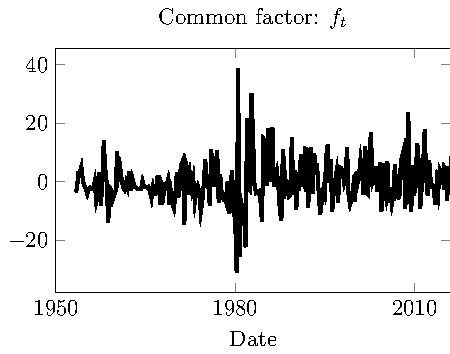
\includegraphics[width=0.5\textwidth]{figdata/body/factor.pdf}}\subfloat{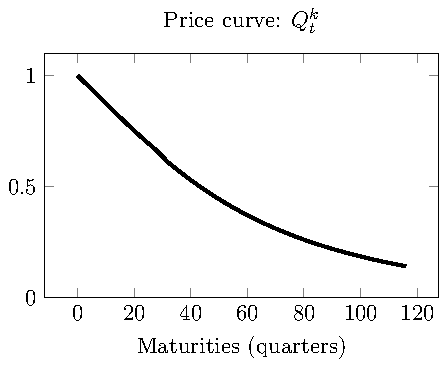
\includegraphics[width=0.5\textwidth]{figdata/body/pricecurve.pdf}}
	
	\hspace{4cm}{\scriptsize{}(a)}\hspace{7.3cm}{\scriptsize{}(b)\bigskip{}
	}%

	\end{minipage}
	
	\noindent %
	\noindent\begin{minipage}[t]{1\columnwidth}%
	{\footnotesize{}{}{}{}{}{}{}}{\scriptsize{}{}Notes: The left
	panel plots the time series for the common factor. The common factor
	is extracted as the first principal component from observed returns,
	the government surplus, output, and the risk-free rate. The right
	panel plots the bond price curve. We use data from Gurkaynak et al.
	for the period 1952-2017 to compute average yields for maturities
	spaced 4 quarters apart and then interpolate the yields.}%
	\end{minipage}
	\end{figure}

	
\begin{comment}
\begin{figure}[H]
\caption{\label{fig:inputs} INPUTS FOR TARGET PORTFOLIO}
\subfloat{\centering

\begin{tikzpicture}       
	\def\myplotFILENAME{figdata/body/factordata.csv}
	\pgfplotstableread[col sep=comma]{\myplotFILENAME}\myplotDataFactor

	\begin{axis}[
				title={Common factor: $f_t$},     
				xlabel={Date},     				
				height=0.25\textheight,
				width=0.5\textwidth,
				scaled x ticks = false,   
				x tick label style={/pgf/number format/.cd, 1000 sep={}},
				xmin=1950,xmax=2016, 	
				xtick={1950,1980,...,2017},
				legend pos=north east, 
				y tick label style={/pgf/number format/.cd, scaled y ticks = false, set thousands separator={}, fixed}
				] 

% Here we plot the data from the CSV file 

	\addplot[line width=1.5pt,color=black]  table[x=datealt, y=factor1] {\myplotDataFactor}; 
%\addlegendentry{$1^{st}$ Factor}
%\addplot[line width=1.5pt,color=orange]  table[x=datealt, y=factor2] {\myplotDataFactor}; 
%\addlegendentry{$2^{nd}$ Factor}
	\end{axis} 
\end{tikzpicture} }\subfloat{\centering

\begin{tikzpicture}       
	\def\myplotFILENAME{figdata/body/feds_mean.csv}
	\pgfplotstableread[col sep=comma]{\myplotFILENAME}\myplotData

	\begin{axis}[     
				title={Price curve: $Q^k_t$},     
				xlabel={Maturities (quarters)}, 
				height=0.25\textheight,
				width=0.5\textwidth,    
				ymin=0, 
				ymax=1.1
				] 
	
% Here we plot the data from the CSV file 
	
	\addplot[line width=1.5pt,color=black]  table[x=Maturities, y=DiscountFactor] {\myplotData}; 
	\end{axis} 
	
 \end{tikzpicture} }

\noindent\begin{minipage}[t]{1\columnwidth}%
\hspace{4cm}{\scriptsize{}(a)}\hspace{7.3cm}{\scriptsize{}(b)\bigskip{}
}%
\end{minipage}

\noindent %
\noindent\begin{minipage}[t]{1\columnwidth}%
{\footnotesize{}{}{}{}{}{}{}}{\scriptsize{}{}Notes: The left
panel plots the time series for the common factor. The common factor
is extracted as the first principal component from observed returns,
the government surplus, output, and the risk-free rate. The right
panel plots the bond price curve. We use data from Gurkaynak et al.
for the period 1952-2017 to compute average yields for maturities
spaced 4 quarters apart and then interpolate the yields.}%
\end{minipage}
\end{figure}
\end{comment}
\begin{comment}
\begin{figure}
\begin{tikzpicture}
\def\myplotFILENAME{figdata/body/factordata.csv}
\pgfplotstableread[col sep=comma]{\myplotFILENAME}\myplotDataFactor

\begin{axis}[     title={Factor},     xlabel={Date},     height=0.25\textheight,width=\textwidth,scaled x ticks = false,   x tick label style={/pgf/number format/.cd, 1000 sep={}}, xmin=1950,xmax=2016, xtick={1950,1980,...,2017},legend pos=north east,       y tick label style={/pgf/number format/.cd,           scaled y ticks = false,           set thousands separator={},           fixed}] 

% Here we plot the data from the CSV file 

\addplot[line width=1.5pt,color=black]  table[x=datealt, y=factor1] {\myplotDataFactor}; 
\addlegendentry{$1^{st}$ Factor}
$\addplot[line width=1.5pt,color=orange]  table[x=datealt, y=factor2] {\myplotDataFactor}; 
$\addlegendentry{$2^{nd}$ Factor}
\end{axis} 
\end{tikzpicture} \caption{Time series for the the common factor}
\end{figure}
 
\begin{figure}
 \begin{tikzpicture} 

\def\myplotFILENAME{figdata/body/feds_mean.csv}
\pgfplotstableread[col sep=comma]{\myplotFILENAME}\myplotData

\begin{axis}[     title={Discount Factor Over Maturities},     xlabel={Maturities (quarters)},     ylabel={Discount Factor},         width=10cm,     height=6cm,     ymin=0, ymax=1.1] 

% Here we plot the data from the CSV file 

\addplot[line width=1.5pt,color=black]  table[x=Maturities, y=DiscountFactor] {\myplotData}; 
\end{axis} 

\end{tikzpicture}

\caption{The figure plots the bond price curve $Q_{T}^{k}=\exp\{-ky_{T}^{k}\}$.
We use data from {[}cite GSK{]} for the period 1952-2017 to compute
average yields $y_{T}^{k}$ for maturities spaced 4 quarters apart
and then interpolate the yields to obtain $Q_{T}^{k}.$}
\end{figure}
\end{comment}

\begin{table}
\begin{centering}
\caption{FACTOR MODEL ESTIMATION (BASELINE)\label{tab: Factor model estimation}}
\medskip{}
 \medskip{}
 %
\begin{tabular}{>{\raggedright}p{0.68cm}>{\centering}p{0.68cm}>{\raggedright}p{0.68cm}>{\raggedright}p{0.68cm}>{\raggedright}p{0.68cm}>{\raggedright}p{0.68cm}>{\raggedright}p{0.68cm}>{\raggedright}p{0.68cm}>{\raggedright}p{0.68cm}>{\raggedright}p{0.68cm}>{\raggedright}p{0.68cm}>{\raggedright}p{0.68cm}>{\raggedright}p{0.68cm}>{\raggedright}p{0.68cm}>{\raggedright}p{0.68cm}}
\hline 
\raggedright{} & \multicolumn{11}{c}{{\tiny{}{}Excess returns $r_{t}^{j}$ for various maturities $j$}} & \multicolumn{3}{l}{}\tabularnewline
\hline 
\raggedright{} & \raggedright{}{\tiny{}{}6m} & \raggedright{}{\tiny{}{}12m} & \raggedright{}{\tiny{}{}18m} & \raggedright{}{\tiny{}{}24m} & \raggedright{}{\tiny{}{}30m} & \raggedright{}{\tiny{}{}36m} & \raggedright{}{\tiny{}{}42m} & \raggedright{}{\tiny{}{}48m} & \raggedright{}{\tiny{}{}54m} & \raggedright{}{\tiny{}{}60m} & \raggedright{}{\tiny{}{}120m} & \raggedright{}{\tiny{}{}$\ln G_{t}$} & \raggedright{}{\tiny{}{}$\ln\Theta_{t}$} & \raggedright{}{\tiny{}{}$f_{t}$}\tabularnewline
\raggedright{}{\scriptsize{}{}$\alpha_{k}$} & {\tiny{}{}0.086} & {\tiny{}{}0.155} & {\tiny{}{}0.220} & {\tiny{}{}0.245} & {\tiny{}{}0.284} & {\tiny{}{}0.315} & {\tiny{}{}0.346} & {\tiny{}{}0.344} & {\tiny{}{}0.372} & {\tiny{}{}0.304} & {\tiny{}{}0.444} & {\tiny{}{}0.005} & {\tiny{}{}0.005} & {\tiny{}{}0.024}\tabularnewline
\raggedright{} & \raggedright{}{\tiny{}{}\vspace{-6mm}
(0.014)} & \raggedright{}{\tiny{}{}\vspace{-6mm}
(0.025)} & \raggedright{}{\tiny{}{}\vspace{-6mm}
(0.033)} & \raggedright{}{\tiny{}{}\vspace{-6mm}
(0.035)} & \raggedright{}{\tiny{}{}\vspace{-6mm}
(0.039)} & \raggedright{}{\tiny{}{}\vspace{-6mm}
(0.039)} & \raggedright{}{\tiny{}{}\vspace{-6mm}
(0.038)} & \raggedright{}{\tiny{}{}\vspace{-6mm}
(0.037)} & \raggedright{}{\tiny{}{}\vspace{-6mm}
(0.037)} & \raggedright{}{\tiny{}{}\vspace{-6mm}
(0.043)} & \raggedright{}{\tiny{}{}\vspace{-6mm}
(0.030)} & \raggedright{}{\tiny{}{}\vspace{-6mm}
(nan)} & \raggedright{}{\tiny{}{}\vspace{-6mm}
(nan)} & \raggedright{}{\tiny{}{}\vspace{-6mm}
(0.501)}\tabularnewline
\raggedright{}{\scriptsize{}{}$\rho_{k}$} & {\tiny{}{}-0.107} & {\tiny{}{}-0.057} & {\tiny{}{}-0.041} & {\tiny{}{}-0.043} & {\tiny{}{}-0.042} & {\tiny{}{}-0.025} & {\tiny{}{}-0.022} & {\tiny{}{}-0.008} & {\tiny{}{}-0.022} & {\tiny{}{}-0.027} & {\tiny{}{}0.003} & {\tiny{}{}1.000} & {\tiny{}{}1.000} & {\tiny{}{}0.000}\tabularnewline
\raggedright{} & \raggedright{}{\tiny{}{}\vspace{-6mm}
(0.043)} & \raggedright{}{\tiny{}{}\vspace{-6mm}
(0.035)} & \raggedright{}{\tiny{}{}\vspace{-6mm}
(0.030)} & \raggedright{}{\tiny{}{}\vspace{-6mm}
(0.025)} & \raggedright{}{\tiny{}{}\vspace{-6mm}
(0.023)} & \raggedright{}{\tiny{}{}\vspace{-6mm}
(0.020)} & \raggedright{}{\tiny{}{}\vspace{-6mm}
(0.018)} & \raggedright{}{\tiny{}{}\vspace{-6mm}
(0.016)} & \raggedright{}{\tiny{}{}\vspace{-6mm}
(0.015)} & \raggedright{}{\tiny{}{}\vspace{-6mm}
(0.015)} & \raggedright{}{\tiny{}{}\vspace{-6mm}
(0.009)} & \raggedright{}{\tiny{}{}\vspace{-6mm}
(nan)} & \raggedright{}{\tiny{}{}\vspace{-6mm}
(nan)} & \raggedright{}{\tiny{}{}\vspace{-6mm}
(nan)}\tabularnewline
\raggedright{}{\scriptsize{}{}$\kappa_{k}$} & {\tiny{}{}0.028} & {\tiny{}{}0.074} & {\tiny{}{}0.118} & {\tiny{}{}0.157} & {\tiny{}{}0.199} & {\tiny{}{}0.230} & {\tiny{}{}0.257} & {\tiny{}{}0.285} & {\tiny{}{}0.306} & {\tiny{}{}0.345} & {\tiny{}{}0.404} & {\tiny{}{}-0.032} & {\tiny{}{}-0.047} & {\tiny{}{}0.000}\tabularnewline
\raggedright{} & \raggedright{}{\tiny{}{}\vspace{-6mm}
(0.002)} & \raggedright{}{\tiny{}{}\vspace{-6mm}
(0.003)} & \raggedright{}{\tiny{}{}\vspace{-6mm}
(0.004)} & \raggedright{}{\tiny{}{}\vspace{-6mm}
(0.004)} & \raggedright{}{\tiny{}{}\vspace{-6mm}
(0.005)} & \raggedright{}{\tiny{}{}\vspace{-6mm}
(0.005)} & \raggedright{}{\tiny{}{}\vspace{-6mm}
(0.005)} & \raggedright{}{\tiny{}{}\vspace{-6mm}
(0.005)} & \raggedright{}{\tiny{}{}\vspace{-6mm}
(0.005)} & \raggedright{}{\tiny{}{}\vspace{-6mm}
(0.005)} & \raggedright{}{\tiny{}{}\vspace{-6mm}
(0.004)} & \raggedright{}{\tiny{}{}\vspace{-6mm}
(0.016)} & \raggedright{}{\tiny{}{}\vspace{-6mm}
(0.008)} & \raggedright{}{\tiny{}{}\vspace{-6mm}
(nan)}\tabularnewline
\raggedright{}{\scriptsize{}{}$\sigma_{k}^{2}$} & {\tiny{}{}0.044} & {\tiny{}{}0.154} & {\tiny{}{}0.267} & {\tiny{}{}0.300} & {\tiny{}{}0.378} & {\tiny{}{}0.384} & {\tiny{}{}0.356} & {\tiny{}{}0.345} & {\tiny{}{}0.341} & {\tiny{}{}0.460} & {\tiny{}{}0.222} & {\tiny{}{}4.231} & {\tiny{}{}1.147} & {\tiny{}{}63.753}\tabularnewline
\raggedright{} & \raggedright{}{\tiny{}{}\vspace{-6mm}
(0.004)} & \raggedright{}{\tiny{}{}\vspace{-6mm}
(0.014)} & \raggedright{}{\tiny{}{}\vspace{-6mm}
(0.024)} & \raggedright{}{\tiny{}{}\vspace{-6mm}
(0.027)} & \raggedright{}{\tiny{}{}\vspace{-6mm}
(0.034)} & \raggedright{}{\tiny{}{}\vspace{-6mm}
(0.034)} & \raggedright{}{\tiny{}{}\vspace{-6mm}
(0.031)} & \raggedright{}{\tiny{}{}\vspace{-6mm}
(0.031)} & \raggedright{}{\tiny{}{}\vspace{-6mm}
(0.030)} & \raggedright{}{\tiny{}{}\vspace{-6mm}
(0.041)} & \raggedright{}{\tiny{}{}\vspace{-6mm}
(0.020)} & \raggedright{}{\tiny{}{}\vspace{-6mm}
(0.375)} & \raggedright{}{\tiny{}{}\vspace{-6mm}
(0.102)} & \raggedright{}{\tiny{}{}\vspace{-6mm}
(5.637)}\tabularnewline
\raggedright{}{\scriptsize{}{}R2} & {\tiny{}{}0.536} & {\tiny{}{}0.698} & {\tiny{}{}0.771} & {\tiny{}{}0.840} & {\tiny{}{}0.870} & {\tiny{}{}0.898} & {\tiny{}{}0.922} & {\tiny{}{}0.938} & {\tiny{}{}0.946} & {\tiny{}{}0.943} & {\tiny{}{}0.979} & {\tiny{}{}0.015} & {\tiny{}{}0.109} & {\tiny{}{}0.000}\tabularnewline
\hline 
\end{tabular}
\par\end{centering}
\noindent %
\noindent\begin{minipage}[t]{1\columnwidth}%
{\footnotesize{}{}{}{}{}{}{}}{\scriptsize{}{}Notes: This table
records the OLS estimates of the factor model (\ref{eq: factor model}).
Standards errors are in parenthesis. The sample for excess returns
and primary surpluses normalized by outputs is 1952-2017. The time
period is a quarter.}%
\end{minipage}
\end{table}

We use this factor model to construct the target portfolio using formula
(\ref{eq: w* TFP}). Since that formula requires interest rates and
returns for horizons beyond the twelve CRSP maturities, we extrapolate
factor loadings and volatilities of missing maturities using exponential
curves of the form $e^{0}-e^{0}\exp\left(-e^{1}j\right)$, where the
coefficient $e^{1}$ captures the slope and the coefficient $e^{0}$
bounds the range of values between $\left[0,e^{0}\right]$. We provide
additional details about the fit and discussion of robustness in online
Appendix \ref{sec:Additional-details-for-section 5}.

To implement formula (\ref{eq: w* TFP}), covariances $\Sigma_{t}$,
$\Sigma_{t}^{G}$, $\Sigma_{t}^{\Theta}$ can be directly constructed
using our observations above. We construct $\Sigma_{t}^{Q}$ using
the relationship $cov_{t}(\ln Q_{t+1}^{k},r_{t+1}^{j})\simeq cov_{t}(r_{t+1}^{k},r_{t+1}^{j})/Q_{t}^{1}.$
Weights $s_{t}^{G}[k],$ $s_{t}^{\Theta}[k]$, and $s_{t}^{Q}[k]$
can be constructed from our estimates since to the appropriate order
of approximation they satisfy $\frac{Q_{t}^{k}\Gamma^{k}G_{t}}{Q_{t}^{1}B_{t}}$,
$\frac{Q_{t}^{k}\Gamma^{k}T_{t}}{Q_{t}^{1}B_{t}}$, and $\frac{Q_{t}^{k+1}\Gamma^{k+1}}{Q_{t}^{1}\sum_{k=1}^{\infty}Q_{t}^{k}\Gamma^{k}}$
where $\Gamma:=\exp(\alpha)$ and $\alpha$ is the growth rate of
log $G$ as well as $\ln\Theta.$ The terms $\{Q_{t}^{k}\Gamma^{k}\}_{k}$
will play an important role in the expressions for the optimal portfolios.
Recall that $Q_{t}^{k}$ is the period-$t$ price of a bond with maturity
$k$ (see Figure \ref{fig:inputs} (b)) so $Q_{t}^{k}\Gamma^{k}$
is the price of that bond adjusted by the expected growth rate $\Gamma^{k}$
that occurs by the time this bond matures. We use $\hat{\beta}_{t}:=1-\frac{1}{\sum_{k=1}^{\infty}Q_{t}^{k}\Gamma^{k}}$
to denote the ``discount factor'' implied by this growth-adjusted
price curve.

Using these observations, we can construct the target portfolio $\omega_{t}^{*}$
for any arbitrary set of bond maturities. We denote the set of available
maturities as $\mathcal{G}$. For most of our discussion, we take
$\mathcal{G}$ to consist of all maturities up to 30 years, which
in our quarterly data specification means $\mathcal{G}=\{1,2,...,120\}$.
This choice is in line with issuance practices of the U.S. government.
We also discuss implications of choosing other sets $\mathcal{G}$.

We present the target portfolio as a sum of two portfolios, $\omega_{t}^{*}=\omega_{t}^{X}+\omega_{t}^{Q}$
where $\omega_{t}^{X}$, $\omega_{t}^{Q}$ have elements 
\begin{align}
\begin{split}\omega_{t}^{X}[j]=\left(\frac{1}{1-\hat{\beta}_{t}}\right)\left(\frac{\kappa_{\Theta}T_{t}-\kappa_{G}G_{t}}{Q_{t}^{1}B_{t}}\right)\left(\frac{\kappa_{j}}{\sigma_{j}^{2}}\chi^{2}\right) & ,\end{split}
\label{eq: components A and X-1}
\end{align}
\begin{equation}
\omega_{t}^{Q}[j]=\left(1-\hat{\beta}_{t}\right)\left(\sum_{\ell\notin\mathcal{G}}Q_{t}^{\ell+1}\Gamma^{\ell+1}\kappa_{\ell}\right)\left(\frac{\kappa_{j}}{\sigma_{j}^{2}}\chi^{2}\right)+\left(1-\hat{\beta}_{t}\right)Q_{t}^{j+1}\Gamma^{j+1},\label{eq: component Q-1}
\end{equation}
and the constant $\chi^{-2}:=\sigma_{f}^{-2}+\sum_{i\in\mathcal{G}}\kappa_{i}^{2}\sigma_{i}^{-2}$.
Portfolios $\omega_{t}^{X},$ $\text{\ensuremath{\omega_{t}^{Q}}}$
have natural economic interpretation. Portfolio $\omega_{t}^{X}$
equals $\Sigma_{t}^{-1}\Sigma_{t}^{G}s_{t}^{G}+\Sigma_{t}^{-1}\Sigma_{t}^{\Theta}s_{t}^{\Theta}$
and is the portfolio that hedges the primary surplus risk $\{T_{t+k}-G_{t+k}\}_{k}$.
Portfolio $\omega_{t}^{Q}=\Sigma_{t}^{-1}\Sigma_{t}^{Q}s_{t}^{Q}$
hedges the interest rate risk.

Formulas (\ref{eq: components A and X-1}) and (\ref{eq: component Q-1})
contain several observations about how these risks are hedged. Equation
(\ref{eq: components A and X-1}) shows how shocks to primary surpluses
are hedged. This expression shows that maturities with higher values
of $\frac{\kappa_{j}}{\sigma_{j}^{2}}$ have a bigger weight in the
portfolio that hedges primary surpluses. This ratio has a following
interpretation. Loading $\kappa_{j}$ captures how much the returns
of bonds of maturity $j$ co-move with a common factor, and $\sigma_{j}^{2}$
captures the volatility of the component of returns that is orthogonal
to the common factor. Thus, $\frac{\kappa_{j}}{\sigma_{j}^{2}}$ is
a measure of how good maturity $j$ is at hedging macroeconomic shocks.
The other parameters in (\ref{eq: components A and X-1}) are scaling
terms: $\frac{\kappa_{\Theta}T_{t}-\kappa_{G}G_{t}}{Q_{t}^{1}B_{t}}$
is the hedgeable part of primary surpluses in period $t$ in the market
value of debt, and $(1-\hat{\beta}_{t})^{-1}$ converts that statistic
into the present value, which under our balanced growth path factor
structure takes a particularly simple form.

Equation (\ref{eq: component Q-1}) shows that the portfolio that
hedges interest rate risk has a related but distinct structure. This
portfolio consists of two terms. The first term on the right hand
side of (\ref{eq: component Q-1}) has a similar structure to the
right hand side of (\ref{eq: components A and X-1}), that is, portfolio
weights depends on the ratio $\frac{\kappa_{j}}{\sigma_{j}^{2}}$
and scaling terms. Importantly, the scaling terms depend only on the
interest rates of the maturities not included in $\mathcal{G}$, that
is, $\left\{ \ell\notin\mathcal{G}\right\} $. So that if $\mathcal{G}$
has maturities for the first 30 years, this term captures fluctuations
in long interest rates beyond the 30 year horizon.

The second term in (\ref{eq: component Q-1}) has a very simple structure
in which holdings of maturity $j$ is proportional to $Q_{t}^{j+1}\Gamma^{j+1}$.
To understand the reason for this structure, and why it is different
from (\ref{eq: components A and X-1}), recall the maturity matching
principle from the discussion of equation (\ref{eq:maturity matching}).
When all maturities are available, the maturity matching principle
said that a good way to hedge interest rate risks was to align the
quantity of debt to the path of expected primary surpluses. With our
balanced growth specification, expected deficits grow at rate $\Gamma$,
and this principle will imply portfolio shares that are proportional
to $Q_{t}^{j+1}\Gamma^{j+1}$.

This discussion highlights several take-aways. First, the target portfolio
must have a component driven by maturity matching. In the context
of a market structure with a cap of the maximum maturity, we denote
the component driven by maturity matching as $\omega_{t}^{mm}[j]\equiv(1-\hat{\beta}_{t})\times\{Q_{t}^{j+1}\Gamma^{j+1}\}_{j}$
for all available maturities $j\in\mathcal{G}$. The deviations of
$\omega_{t}^{*}$ from $\omega_{t}^{mm}$ are determined by quantitative
strength of two forces: the ability of available bonds hedge primary
surpluses and very long interest rates. Second, if we increase the
number of maturities in $\mathcal{G}$, the relative importance of
the second force declines.

We now use our estimation to construct the target portfolio $\omega_{t}^{*}$.
We choose $\mathcal{G}$ to consist of first 30 year maturities and
plot implies $\omega_{t}^{*}$ in Figure \ref{fig: portfolio shares}
(a). For comparison, we also plot the actual U.S. portfolio of government
bonds in 2017. Both graphs show that portfolio shares decline in maturities,
roughly geometrically, but the U.S. portfolio overweights short maturities
and underweights long maturities. Thus, the duration of the target
portfolio is longer. The Macaulay duration, which measures the weighted
average time to maturity of cash flows, is approximately 5 years for
the U.S. portfolio and 9.6 years for the target portfolio.

Panel (b) of Figure \ref{fig: portfolio shares} sheds light on what
determines quantitative properties of $\omega_{t}^{*}$. Here we plot
component portfolios $\omega_{t}^{Q}$, $\omega_{t}^{X}$, and $\omega_{t}^{mm}$.
This panel shows that $\omega_{t}^{*}$ is extremely similar to $\omega_{t}^{mm}$.
This result comes from the interaction of two forces. The interest
rate risk hedging portfolio $\omega_{t}^{Q}$ has a bit longer duration
than $\omega_{t}^{mm},$ since longer maturities are better at hedging
interest rate risk beyond the 30 year horizon. At the same time $\omega_{t}^{X}$
has negative weights, reflecting the fact that primary surpluses co-move
negatively with returns in the data, and so negative holdings of those
bonds hedge risk.\footnote{For instance, consider states when tax revenues are low. The negative
covariance between long maturity rates and primary surplus means that
long interest rates will be high in those states. Thus, issuing fewer
long duration bonds is helpful because it offsets the loss in tax
revenues with lower debt service costs without raising distortionary
taxes. The negative (or long) positions in $\omega_{t}^{X}$ capture
this tradeoff.} These two effects approximately cancel out so that $\omega_{t}^{*}$
resembles portfolio $\omega_{t}^{mm}$.

Another observation from Figure \ref{fig: portfolio shares} is that
bonds offer modest ability for the government for hedging of the primary
surpluses. The ratio $\frac{\kappa_{j}}{\sigma_{j}^{2}}$ peaks for
medium-duration maturities but even then the role of these bonds in
hedging primary surpluses is fairly small. One way to quantify the
importance of hedging of interest rate risk vs primary surplus risk
is to compute shares $\frac{\left\Vert \omega_{t}^{Q}\right\Vert _{1}}{\left\Vert \omega_{t}^{Q}\right\Vert _{1}+\left\Vert \omega_{t}^{X}\right\Vert _{1}}$
and $\frac{\left\Vert \omega_{t}^{X}\right\Vert _{1}}{\left\Vert \omega_{t}^{Q}\right\Vert _{1}+\left\Vert \omega_{t}^{X}\right\Vert _{1}}$,
where $\left\Vert \cdot\right\Vert _{1}$ denotes the $l_{1}$ norm
(i.e., the sum of absolute values). Using this metric, the importance
of hedging of interest rate risk is approximately 85\% in the target
portfolio, and the importance of hedging of the primary surplus risk
is 15\%. The poor ability of bonds to hedge primary surplus risk should
not be surprising given the observations in Table \ref{tab:covariances}.
As we highlighted in that table, covariances of returns on bonds with
macroeconomic variables are fairly low, especially compared to the
volatility of those returns.

\begin{figure}[H]
\caption{\label{fig: portfolio shares} TARGET PORTFOLIO, COMPONENTS, AND U.S.
PORTFOLIO}
\subfloat{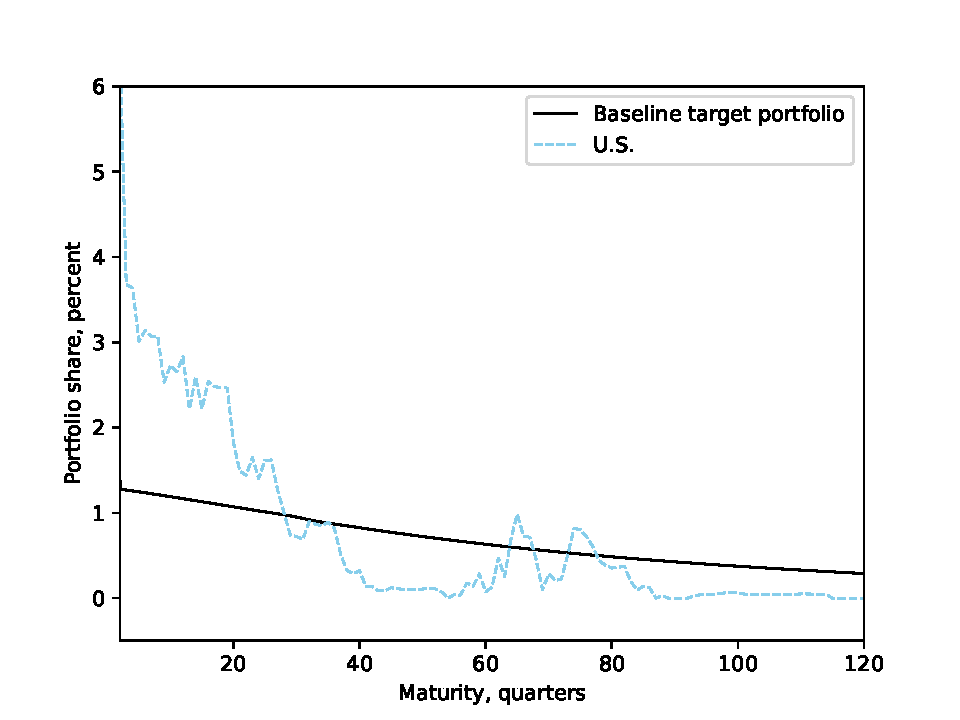
\includegraphics[width=0.5\textwidth]{figdata/body/opt_us}}\subfloat{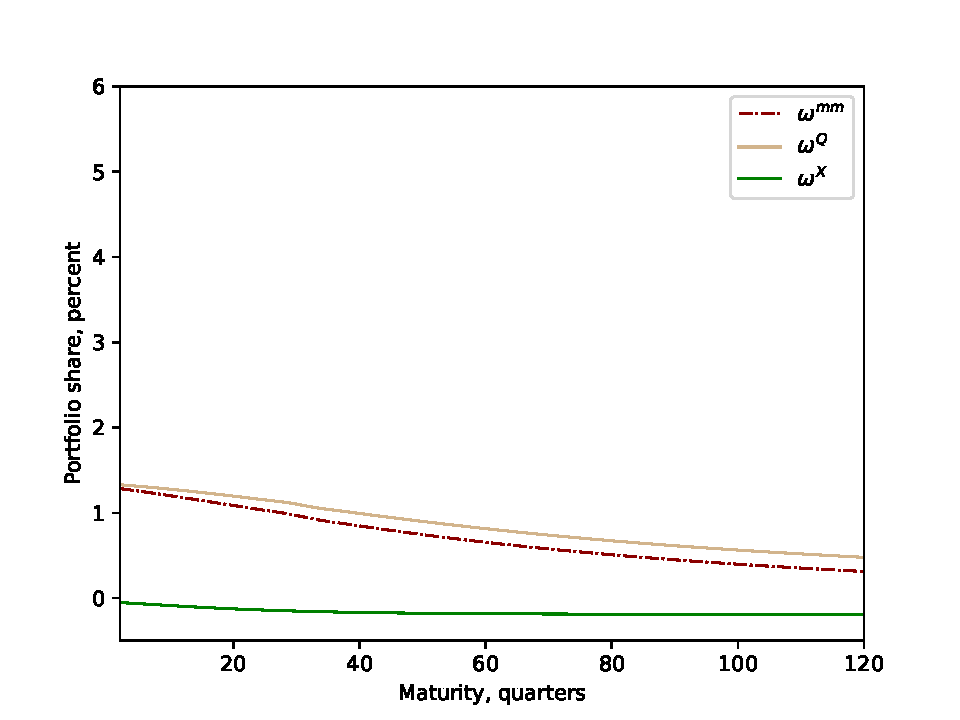
\includegraphics[width=0.5\textwidth]{figdata/body/main_comp}}

\noindent\begin{minipage}[t]{1\columnwidth}%
\hspace{4cm}{\scriptsize{}(a)}\hspace{7.3cm}{\scriptsize{}(b)\bigskip{}
}%
\end{minipage}

\noindent\begin{minipage}[t]{1\columnwidth}%
{\footnotesize{}{}{}{}{}{}{}}{\scriptsize{}{}Notes: Portfolio
shares of securities with maturities from 2 quarters to 120 quarters.
In panel (a) we plot the target portfolio and compare it to the 2017
U.S. debt portfolio. In panel (b) we plot the maturity matching portfolio
$\omega_{t}^{mm}$ and the two components of the target portfolio
that hedge interest rate risk $\omega_{t}^{Q}$, and primary surplus
risk $\omega_{t}^{X}$, respectively.}%
\end{minipage}
\end{figure}

We next discuss the role of certain assumptions made in the baseline
calculations.

\paragraph*{Multifactor models}

Our baseline empirical specification (\ref{eq: factor model}) assumes
that there is one factor $f_{t}$. The bond pricing literature going
back to the seminal work of \citet{litterman1991common} showed that
a small number of factors explains vast fraction of volatility of
bond returns but typically uses more than one factor.\footnote{For example, \citeauthor{litterman1991common} used a 3 factor model
for bond excess returns. They show that the first three principal
components of bond returns explained more than 96\% of variation in
their sample. Based on the shape of the factor loadings, they interpreted
the factors as\emph{ level, slope, }and\emph{ curvature.}} We now discuss a multi-factor extension of our factor model (\ref{eq: factor model}).

Our general multifactor specification replaces $\kappa_{\iota}f_{t}$
with $\sum_{m}\kappa_{m,\iota}f_{t}^{m}$ where $m$ is the index
for factors. In this section, we present the result for a two-factor
model where factors correspond to the first two principal components
of the observed bond returns, the government surplus, output, and
the risk-free rate. This two-factor specification explains over 98\%
of bond excess returns.\footnote{We experimented with adding more factors and did not find any meaningful
changes in the results.} 

We relegate most of the details about the estimation to online Appendix
\ref{sec:Additional-details-for-section 5}and briefly summarize the
main takeaways here. The second factor is less volatile as compared
to the first factor. The factor loadings on both factors are statistically
significant for all the returns but have different shapes as a function
of maturity. The loadings on the first factor are monotonically increasing
in maturity, while those on the second factor are hump shaped. This
corresponds to the level and curvature factors in the \citet{litterman1991common}
terminology. Finally, only the first factor has statistically significant
loadings for $\ln G_{t}$ and $\ln\Theta_{t}$. Overall, while the
two factors are necessary for a more accurate description of returns,
the second factor matters little for spending and tax revenue risk.

The multi-factor specification preserves the tractability of our one-factor
model. One can still derive the analogue of expressions (\ref{eq: components A and X-1})
and (\ref{eq: component Q-1}) and those expressions capture the same
economic forces that we emphasized in our baseline specification.
We plot the target portfolio $\omega_{t}^{*}$ implied by the two-factor
model in Figure \ref{fig:mf}(a).\footnote{Here and in the rest of the section, we follow a convention of setting
statistically insignificant regression coefficients to zero when we
implement our formulas.} For comparison, we also plot the U.S. portfolio and the growth-adjusted
price curve $\omega_{t}^{mm}$ that are the same as in Figure \ref{fig:mf}(a).
The two-factor specification slightly shifts portfolio towards shorter
maturities but the overall difference from the baseline specification
is small, with second factor reducing the Macaulay duration from 9.6
to 9.5 years.

In our empirical specification, we built on the\textbf{ }work of \citet{litterman1991common}
and others (for instance, \citet{campbell1998econometrics}, \citet{CochranePiazzesiAER2005},
and \citet{LudvigsonNgRFS2009}) who express bond returns as being
driven by factors common to all maturities and the residuals that
are maturity specific. A particularly convenient feature of this approach
is that the covariance matrix is easily invertible. There exists another
tradition in finance, the so-called affine term structure literature,
that assumes that it is the stochastic discount factor process that
is driven by a small number of factors, and then uses that process
to derive prices and returns of bonds of various maturities (see,
e.g., \citealp{dai2000specification}, \citealp{piazzesi2010affine}).
This approach uses no maturity specific shock $\varepsilon_{t}^{j}$,
so the covariance matrix $\Sigma_{t}$ is not invertible, which implies
that there are multiple optimal portfolios. We assess the role of
idiosyncratic shocks $\varepsilon_{t}^{j}$ in our setting, by sending
the estimated $\sigma_{j}^{2}\to0$ for each $j$ and kept the factor
loadings $\{\kappa_{m,\iota}\}_{m,\iota}$ at their estimated values.
We report our findings in panel (b) of Figure \ref{fig:mf}. This
figure shows that the limiting target portfolio is quite similar to
the target portfolio computed using the estimated $\{\sigma_{j}^{2}\}_{j}$.
This is not surprising given that the orthogonal variation captures
less than 2\% of the variation in returns.

\begin{figure}[H]
\begin{centering}
\caption{\label{fig:mf} ROLE OF MULTIPLE FACTORS}
\par\end{centering}
\subfloat{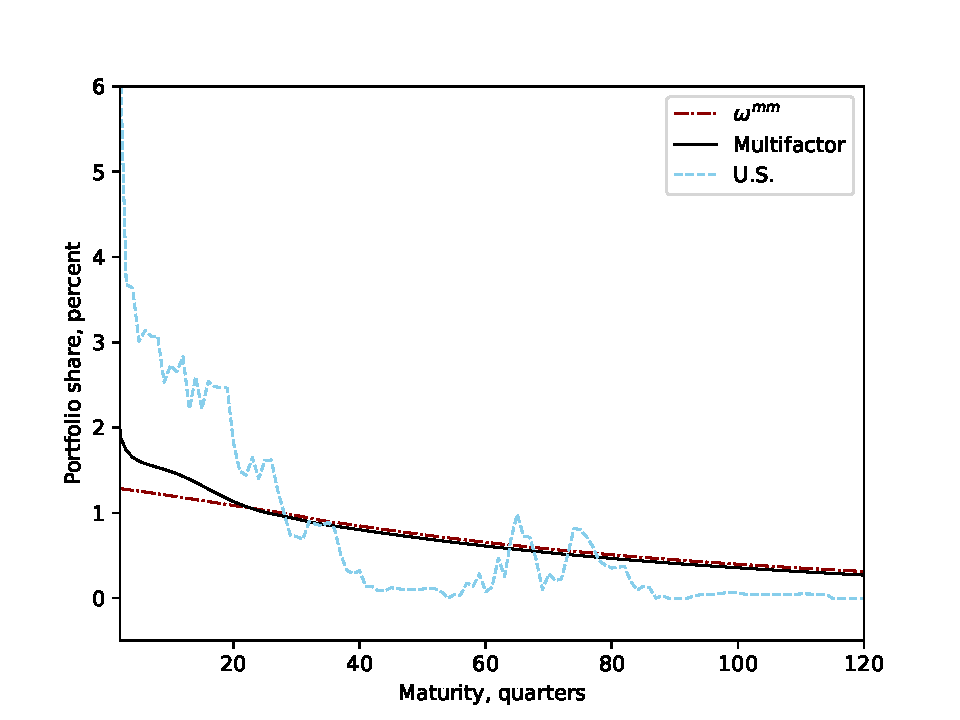
\includegraphics[width=0.5\textwidth]{figdata/body/multifactor}}\subfloat{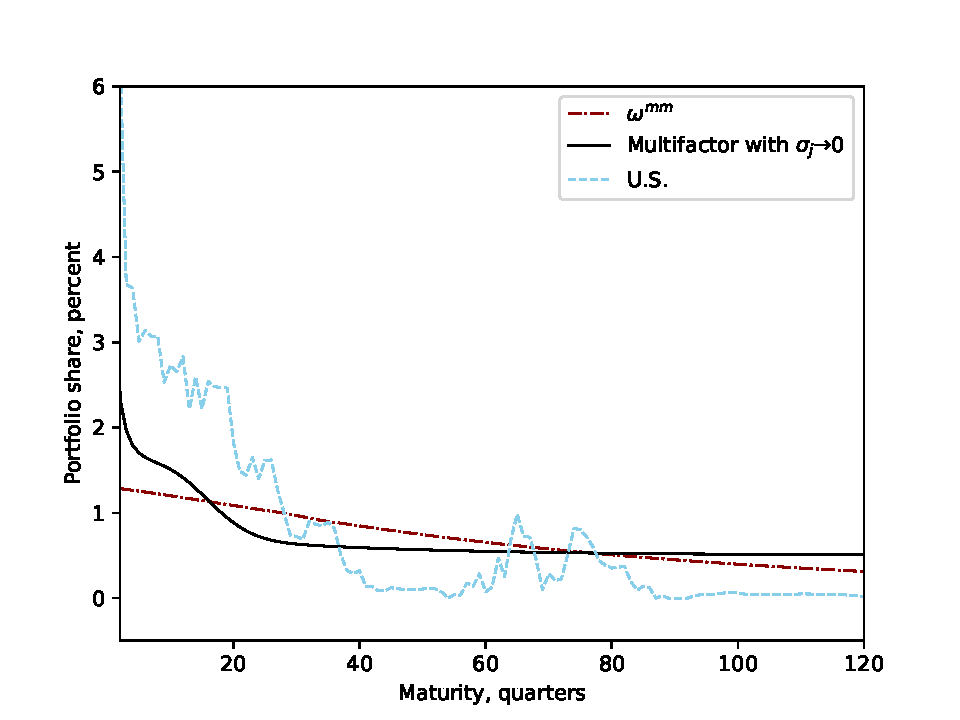
\includegraphics[width=0.5\textwidth]{figdata/body/noise}}

\noindent\begin{minipage}[t]{1\columnwidth}%
\hspace{4cm}{\scriptsize{}(a)}\hspace{7.3cm}{\scriptsize{}(b)\bigskip{}
}%
\end{minipage}

\noindent\begin{minipage}[t]{1\columnwidth}%
{\footnotesize{}{}{}{}{}{}{}}{\scriptsize{}{}Notes: Portfolio
shares of securities with maturities from 2 quarters to 120 quarters.
In panel (a) we compare the maturity matching portfolio $\omega_{t}^{mm}$
to the target portfolio with multiple factors and the U.S. debt portfolio.
In panel (b) we compare the target portfolio with multiple factors
to the limiting target portfolio as send the loadings on idiosyncratic
components $\sigma_{j}^{2}\to0$.}%
\end{minipage}
\end{figure}


\paragraph*{Departures from stationarity}

The baseline factor model assumed stationarity implying that expected
deficits and output grow at a constant rate and covariances are constant.
In online Appendix \ref{sec:Additional-details-for-section 5}, we
discuss several departures from stationarity. Here we summarize the
main results.

First, we turn on the autoregressive components in dynamic factor
model. The optimal portfolio is largely same with these changes. This
is because the excess returns are not very autocorrelated so the estimated
$\rho_{f}$ is close to zero. 

Next we investigate predictability in drivers of primary deficits.
First, we estimate the top equation of (\ref{eq: factor model}) with
a more flexible autoregressive structure. We cannot reject that spending
and TFP are unit roots. However, economies sometimes experience transitory
increases in spending levels. For instance, the public spending during
the COVID-19 pandemic represents such a case. Our expressions for
the target portfolio provide guidance on how the optimal portfolio
should respond to these temporary shocks. In online Appendix \ref{sec:Additional-details-for-section 5},
we consider several experiments with unexpected transitory increases
in spending at date $t$ parameterized by the size of the initial
impulse and the speed of mean reversion.

The general pattern is that after a transitory increase in spending,
the target portfolio ``tilts'' with lower holdings of short maturity
debt and higher holdings of long maturity debt. For a given debt level,
high transitory spending leads to lower primary surpluses in the short-run
and higher primary surpluses in the long run. The maturity matching
motive implicit in the inter-temporal weights on the interest rate
hedging component calls for down-weighting maturities when expected
surpluses are low and shift the portfolio towards longer maturities
when primary surpluses are high.

We also allow for time-varying covariances which we estimate using
a Generalized Autoregressive Conditional Heteroskedasticity (GARCH)
structure. With heteroskedastic shocks, there is in-sample variation
of the covariances and this would generate variation in portfolios
even if we kept $\left(G_{t},\left\{ Q_{t}^{k}\right\} _{k}\right)$
unchanged. However, we find that the portfolios are quite stable.
The is because the time-varying volatility of the common factor shows
up in both the covariances in returns with spending, tax revenues
and the covariances of returns with each other. Since the optimal
portfolio depends on the ratio of these two covariances, the effect
of time-varying risk is muted in how it affects the target portfolio.

\subsection{Price effects \label{subsec:Price-Effects}}

In our previous discussion, we used equation (\ref{eq: w* TFP}) that
implicitly assume that prices of government bonds do not depend on
bond supplies. A large empirical finance literature (see \citet{KrishnamurthyVissingJorgensenJPE2012},
\citet{GreenwoodVayanosRFS2014} and more recently \citet{mian2022goldilocks})
has documented that changes in supply of bonds affect their prices.
In this section, we use empirical estimates of price responses to
evaluate optimal portfolio formation with price effects. For quantitative
evaluation, we will use the generalization of the setup from Section
\ref{sec: price impact} that allows for price effects for bonds of
all maturities.\footnote{See online Appendix \ref{sec:Additional-details-for extentions} for
the exact formulas and more details.}

To compute the optimal portfolio with price effects, we need to estimate
equation (\ref{eq: price response}) which includes nonlinear functions
$\left\{ \varphi_{k,t}\left(\tilde{B}_{t}^{k}\right)\right\} _{k}$.
Following the discussion from Section \ref{sec: price impact}, we
assume that $\left\{ \varphi_{k,t}\right\} _{k}$ are affine functions
of the face value of outstanding debts and thus semi-elasticities
$\left\{ \varphi_{k,t}^{\prime}\right\} _{k}$ are constants. We then
leverage estimates from existing literature to recover these constants.

There is a growing empirical finance literature that estimates semi-elasticities
$\left\{ \frac{\partial\ln\text{yields}_{t}^{k}}{\partial\text{Bond supply}_{t}}\right\} _{k}$,
which capture the effect of changes in bond supply on bond yields
of different maturities. These elasticities are obtained using various
instrumental variable designs that capture exogenous supply-shifters.
A common finding is that these elasticities are positive and increasing
in maturities. To incorporate price effects, in principle, we need
estimates of semi-elasticities $\left\{ \frac{\partial\ln\text{yields}_{t}^{k}}{\partial\tilde{B}_{t}^{k}}\right\} _{k}$
for all $k$, but typically the literature provides such estimates
only measures of total supply such as in total debt in \citet{KrishnamurthyVissingJorgensenJPE2012}
or maturity-weighted debt in \citet{GreenwoodVayanosRFS2014}. Under
the assumption that the portfolio shares are constant when total debt
changes, we can back out semi-elasticities we need to construct price
effects. In online Appendix \ref{sec:Additional-details-for-section 5},
we use this assumption and estimates from \citet{GreenwoodVayanosRFS2014}
to construct the matrix $\Lambda_{t}.$

We can now describe the optimal portfolio of public debts with price
effects. We use a version of formula (\ref{eq: w* price}) that relaxes
the assumption that demand for risk-free bond is perfectly elastic.\footnote{See equation (\ref{eq: price effects with costly bond without h})
in online Appendix \ref{sec:Additional-details-for extentions}.} Formula (\ref{eq: w* price}) and its generalizations prescribes
a non-trivial dependence of portfolio $\omega_{t}$ on portfolio $\omega_{t-1}.$
To facilitate comparisons with the target portfolio $\omega_{t}^{*}$
we focus on $\omega^{ss}=\lim_{t\to\infty}\omega_{t}$, or the the
long run portfolio when the transition dynamics have settled down.\footnote{For computing the long run portfolio, we need specify how matrices
$D_{t}$ and $\Lambda_{t}$ evolve with $t$. Under the assumption
that $\left\{ Q_{t}^{k}\right\} $ are set to sample averages and
implication of government optimality that $\mathbb{E}_{t}\tau_{t+\ell}=\tau_{t}$,
we have $D_{t+\ell}=\Gamma^{\ell}D_{t}$ where $\Gamma$ is the growth
rate of output along the balanced growth path. Under our assumption
that the semi-elasticities $\varphi_{k,t}^{\prime}$ are constants,
and we have $\Lambda_{t+\ell}=\Lambda_{t}.$}

\begin{comment}
\[
\omega_{t}\approx\omega_{t}^{*}-\frac{d_{t}}{Y_{t}}\Sigma_{t}^{-1}\Lambda_{t}^{QE}\left(\omega_{t}-\omega_{t-1}^{+}\right),
\]
where $d_{t}=\frac{Y_{t}\sum_{k=1}^{\infty}Q_{t}^{k}}{\left(Q_{t}^{1}\right)^{2}}\frac{\xi^{2}\left(\tau_{t}\right)}{-\xi^{\prime}\left(\tau_{t}\right)}$
and $\omega_{t-1}^{+}$ be the vector of $\{Q_{t}^{k}\widetilde{B}_{t-1}^{k+1}/B_{t}\}_{k\neq1}$.
We can write this as $\overline{\omega}_{T-1}^{+,k}=\underbrace{\frac{Q_{t}^{k}}{Q_{t-1}^{k+1}}}_{1/Q^{rf}}\times\underbrace{\frac{Q_{t-1}^{k+1}\widetilde{B}_{t-1}^{k+1}}{B_{t-1}}}_{\omega_{T-1}\left[k+1\right]}\times\underbrace{\frac{B_{t-1}}{B_{t}}}_{1/\Gamma}$

Lets do the stationary case in which $\frac{\overline{Q}_{T}^{i}}{\overline{Q}_{T-1}^{i+1}}\frac{\overline{B}_{T-1}}{\overline{B}_{T}}=\frac{1}{\Gamma Q^{0}}$,
$\frac{d_{t}}{Y_{t}}=-\left(\sum_{k=1}^{\infty}\mathbb{E}Q_{t}^{k}\right)\frac{\xi^{2}\left(\tau\right)}{\xi^{\prime}\left(\tau\right)}$,
and $\Sigma_{t}^{-1}\Lambda_{t}^{QE}=\Sigma^{-1}\Lambda^{QE}$. First
note that we can write the $\omega^{+}$ portfolio as 
\[
\omega_{T-1}^{+}=\underbrace{\left[\begin{array}{cccc}
0 & \frac{1}{\Gamma Q^{0}} & 0 & ...\\
0 & 0 & \frac{1}{\Gamma Q^{0}} & ...\\
.. & ... & ... & ...
\end{array}\right]}_{L^{+}}\omega_{T-1}
\]
and then compute the limiting portfolio as 
\begin{align*}
\omega^{lim} & \approx\omega^{*}-d\Sigma^{-1}\Lambda\left(\omega^{lim}-L^{+}\omega^{lim}\right)\\
\omega^{lim} & \approx\omega^{*}-d\Sigma^{-1}\Lambda\left(I-L^{+}\right)\omega^{lim}\\
\omega^{lim}+d\Sigma^{-1}\Lambda\left(I-L^{+}\right)\omega^{lim} & \approx\omega^{*}\\
\left[I+d\Sigma^{-1}\Lambda\left(I-L^{+}\right)\right]\omega^{lim} & \approx\omega^{*}\\
\omega^{lim} & \approx\left[I+d\Sigma^{-1}\Lambda\left(I-L^{+}\right)\right]^{-1}\omega^{*}
\end{align*}
\end{comment}


\paragraph*{Optimal Portfolio}

Figure \ref{fig: portfolio shares PE} panel (a) reports the optimal
steady state portfolio $\omega^{ss}$ in our preferred habitat model
and compares it to the target portfolio in the Section \ref{sec: target portfolio}.
We see that the optimal portfolio with price effects sits in between
the optimal portfolio without price effects and the observed U.S.
portfolio.

With price effects, the government faces an additional trade-off when
issuing longer maturities relative to hedging motives. As discussed
in Section \ref{sec: target portfolio}, issuing long maturities helps
hedge interest rate risk, but it requires constant rebalancing due
to a cap on the maximum maturity. For instance, the optimal portfolio
without price effects that we computed in Section \ref{sec: target portfolio}
uses all available maturities. Since the maximum maturity is 30 years,
to maintain that portfolio, every period the government has to issue
new 30 year bonds. Our estimates of price effects suggest that long
bonds are expensive to reissue. Thus, to economize the cost of issuances,
the optimal portfolio with price effects tilts towards shorter maturities
and away from longer maturities. For our calibration, the Macaulay
duration of the optimal portfolio is $6.15$ years. This duration
is still higher than the U.S. debt portfolio which is about $5$ years
but lower than the duration of the optimal portfolio ignoring the
price effects which was $9.6$ years.

This discussion also suggests that the tradeoff between costly reissuances
and hedging depends on the cap on the maximum maturity. The ability
to issue longer maturities mechanically reduces the amount of debt
that needs to be rebalanced, and has an additional benefit of better
hedging of interest rate risk as highlighted by the discussion of
equation (\ref{eq: component Q-1}) in the previous section. Thus,
one should expect the optimal portfolio with and without price effects
to come closer as we expand the set of available maturities. We verify
this in panel (b) of Figure \ref{fig: portfolio shares PE} where
we plot the optimal portfolios assuming $N=200$ or 50 years. The
difference in Macaulay durations of the optimal portfolio with and
without price effects with $N=200$ is only 6 months. %
\begin{comment}
The economics underlying this outcome flows from discussion at the
end of Section \ref{sec: price impact} and the discussion of equation
(\ref{eq: component Q-1}): As the number of available maturities
grow, $\omega_{t}^{*}$ close to portfolio that hedges interest rate
risk, so price responses have small effects on the optimal portfolio.
\end{comment}

\begin{comment}
the definition if $\omega_{t-1}^{+}$ is$\{Q_{t}^{k}\widetilde{B}_{t-1}^{k+1}/B_{t}\}_{k\neq1}$.
If $t-1$ we had $\omega_{t-1}=\omega_{t}^{mm}$, then 
\[
\widetilde{B}_{t-1}^{k+1}=\mathbb{E}_{t-1}X_{t+k}
\]
and thus 
\[
B_{t}\omega_{t-1}^{+}[k]=Q_{t}^{k}\mathbb{E}_{t}X_{t+k}=B_{t}\omega_{t}^{mm}[k]
\]
\end{comment}

\begin{figure}[H]
\begin{centering}
\caption{\label{fig: portfolio shares PE} OPTIMAL PORTFOLIO WITH PRICE EFFECTS}
\par\end{centering}
\begin{centering}
\subfloat{\centering{}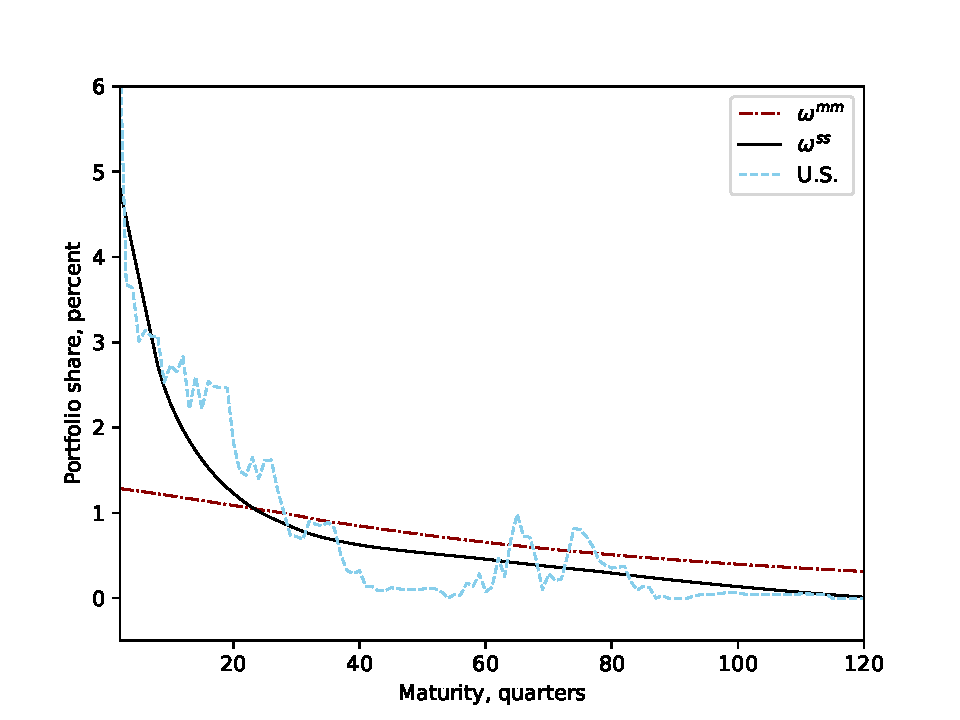
\includegraphics[width=0.5\textwidth]{figdata/body/opt_pe}}\subfloat{\centering{}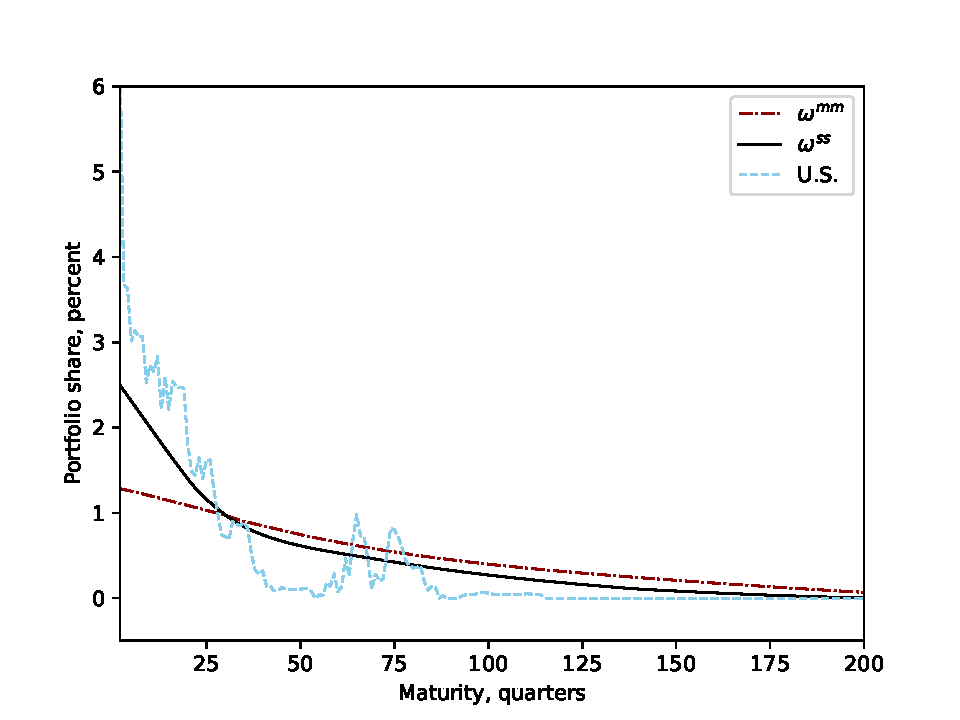
\includegraphics[width=0.5\textwidth]{figdata/body/opt_pe_N50}}
\par\end{centering}
\noindent\begin{minipage}[t]{1\columnwidth}%
\hspace{4cm}{\scriptsize{}(a)}\hspace{7.3cm}{\scriptsize{}(b)\bigskip{}
}%
\end{minipage}

\noindent\begin{minipage}[t]{1\columnwidth}%
{\footnotesize{}{}{}{}{}{}{}}{\scriptsize{}{}Notes: Portfolio
shares of securities with maturities from 2 quarters to $N$ quarters.
In panel (a) we set $N=120$ and plot the optimal portfolio with price
effects and compare it to the maturity matching portfolio $\omega_{t}^{mm}$
and the U.S. debt portfolio. In panel (b) we repeat the exercise with
$N=200$ quarters. The price effects are calibrated using \citet{GreenwoodVayanosRFS2014}.}%
\end{minipage}
\end{figure}


\subsection{Household heterogeneity\label{subsec:Imperfect-substitutes-empirical}}

To get a sense of the magnitude of the inequality-hedging portfolio
in the optimal portfolio (\ref{optimal portfolio with heterogenity}),
we use the following back-of-the-envelope calculation. Assume that
a household type $h=L$ represents a group of individuals who are
in the left-tail (or bottom $L$ percentile) of the income distribution,
and that the planner sets $\mu_{L,t}=1$. Then $\Sigma_{t}^{ineq}[j,k]$
depends on how the income share of the bottom $L$ percentile covaries
with returns. We can use our factor model in equation (\ref{eq: factor model})
with an additional equation 
\[
\ln\frac{Y_{t}}{y_{L,t}}=\alpha_{ineq}+\rho_{ineq}\ln\frac{Y_{t-1}}{y_{L,t-1}}+\kappa_{ineq}f_{t}+\sigma_{ineq}\epsilon_{t}^{ineq},
\]
to parameterize $\Sigma_{t}^{-1}\Sigma_{t}^{ineq}$ with two new objects:
$\kappa_{ineq}$, a loading of inequality on the common factor, and
$\rho_{ineq}$, the first-order autocorrelation in a measure of inequality. 

We set $L=25\%$ and use income share data from \citet{GuvenenEtAllJPE2014}
to obtain $\kappa_{ineq}=0.002$ and $\rho_{ineq}=0.92$.\footnote{\citet{GuvenenEtAllJPE2014} use SSA data and provide means as well
as quantiles of labor earnings at an annual frequency from 1978-2011.
We first detrend the raw measure of inequality and then project it
onto the unemployment rate to obtain a quarterly inequality series.
We estimated $\kappa_{ineq}$ and $\rho_{ineq}$ by using OLS. } Our estimates suggest that the adjustment to the target portfolio
is very small, and this comes from a weak correlation of bond returns
with movements in income inequality.

To get a sense of what heterogeneous trading frictions mean for the
duration of an optimal portfolio, we capture the differences in consumption
risk using a parsimonious formulation that sets $\ln\left(M_{\mathbb{N},t+k}\right)=(1+\psi)\ln\left(M_{\mathbb{T},t+k}\right)$;
the scalar parameter $\psi$ is intended to measure strength of trading
frictions. When non-traders face more risk, so that multiplier $\ln\left(M_{\mathbb{N},T+t}\right)$
is more volatile than $\ln\left(M_{\mathbb{T},t+k}\right)$, the parameter
$\psi>0$. Substituting into the definition of $\Sigma_{t}^{M}$ and
using the counterpart of the traders' Euler equation we get 
\[
\Sigma_{t}^{M}[k,j]=\psi\mu_{\mathbb{N},k}\left[\mathbb{E}_{t}r_{t+1}^{j}-\text{cov}_{t}\left(\ln Q_{t+1}^{k-1},r_{t+1}^{j}\right)\right],
\]
where all the terms in the square bracket on the right-hand side can
be measured from return data that we used in Section \ref{sec: target portfolio}.
In online Appendix \ref{sec:Additional-details-for-section 5}, we
use estimates from factor model (\ref{eq: factor model}) to quantify
those terms for a special case in which the government trades a risk-free
and a growth-adjusted consol and verify that imperfect risk sharing
lengthens the optimal maturity.

\section{Debt portfolios in neoclassical models\label{sec: Comparing to neoclassical}}

Several papers including \citet{LucasStokeyJME1983}, \citet{zhu1992optimal}
and \citet{Chari_etalJPE1994}, study optimal public portfolios in
``neoclassical'' models with complete markets and a representative
agent who has time separable expected utility preferences over consumption
and leisure. \citet{AngeletosQJE2002} showed that it is both feasible
and optimal for a government with access to a sufficiently big set
of zero coupon bonds to implement a complete market allocation. He
derived explicit expressions for the required portfolio. \citet{BueraNicolini_etalJME2004}
and \citet{FarhiJPE2010}) found that plausible calibrations of the
neoclassical model requires an optimal portfolio with huge long and
short positions.\footnote{\citet{Lustig_etalJME2008} study a nominal version of the neoclassical
model and impose short-selling as well as maximum maturity restrictions
on the government portfolio. They find that these restrictions are
binding and that an optimal portfolio issues debt almost exclusively
in the maximal maturity bond.} Those portfolios differ markedly from the simple portfolio that we
obtained in Section \ref{sec: target portfolio}.

In this section, we want to understand sources of those differences.
We also want to see how well our simple statistical rules for forming
an optimal portfolio perform in environments where some of the assumptions
used to derive our rules are violated, e.g., absence of income and
price effects.\footnote{In online Appendix \ref{sec:Closed-Economy}, we extend our methods
to study the target portfolio in a closed economy.} We follow \citet{BueraNicolini_etalJME2004} and assume that households
are identical, and that they maximize $\mathbb{E}_{0}\sum_{t=0}^{\infty}\beta^{t}\left[\frac{C_{t}^{1-1/IES}}{1-1/IES}-\frac{Y_{t}^{1+1/\gamma}}{1+1/\gamma}\right]$.
The economy is closed, households and the government trade securities
that are in in zero net supply, and the government chooses issuances
and taxes, bond sales and purchases to finance an exogenous stochastic
government expenditure process. This economy satisfies all of the
conditions that underly our benchmark economy except that it is closed
and that income effects are present.

We first construct an optimal bond portfolio using standard numerical
methods. We call this the \emph{theoretical} optimal portfolio. We
follow \citet{BueraNicolini_etalJME2004} and set $IES=1/2$ and $\gamma=1$.
We assume that $\ln G_{t}$ follows an AR(1) process and calibrate
the mean, variance, and first-order autocorrelation of this process
to match the primary surplus to GDP ratio in the U.S. data. We discretize
this AR(1) process by confining possible realizations to be on a grid
with 20 points. We set the initial level of debt to be four times
(quarterly) output in a corresponding complete market economy.\footnote{See online Appendix \ref{sec:appendix neoclassical portfolios } for
detail on how we compute the complete market allocation and the theoretical
portfolio.}

Since the Markov state $s^{t}$ can take 20 possible values, results
of \citet{AngeletosQJE2002} imply that an optimal allocation can
be achieved using only the bonds with the first 20 maturities. We
use formulas that Angeletos derived in Corollary to his Theorem 1
to compute that optimal portfolio and report it in the green line
in Figure \ref{fig: Government-portfolio-shares_Angeletos_and_us}.\footnote{Actually, there are 20 different portfolios, one for each possible
value of $G$. Here we plot portfolio for one of the middle values
$\left(s=10\right)$ of realizations of $G$ for concreteness, but
it is representative of the portfolio shapes in all other states.} By construction, the ratio of the total market value debt to annual
GDP is close to 1, but this conceals large variations in market values
of positions at specific maturities. Consistent with findings of Buera
and Nicolini, our optimal portfolio exhibits huge long-short positions
and variations in them across Markov states. Market values of bonds
of a given maturity can range \emph{several thousand times} annual
GDP.

\begin{figure}
\centering\caption{\label{fig: Government-portfolio-shares_Angeletos_and_us} COMPARISON
TO NEOCLASSICAL PORTFOLIOS}
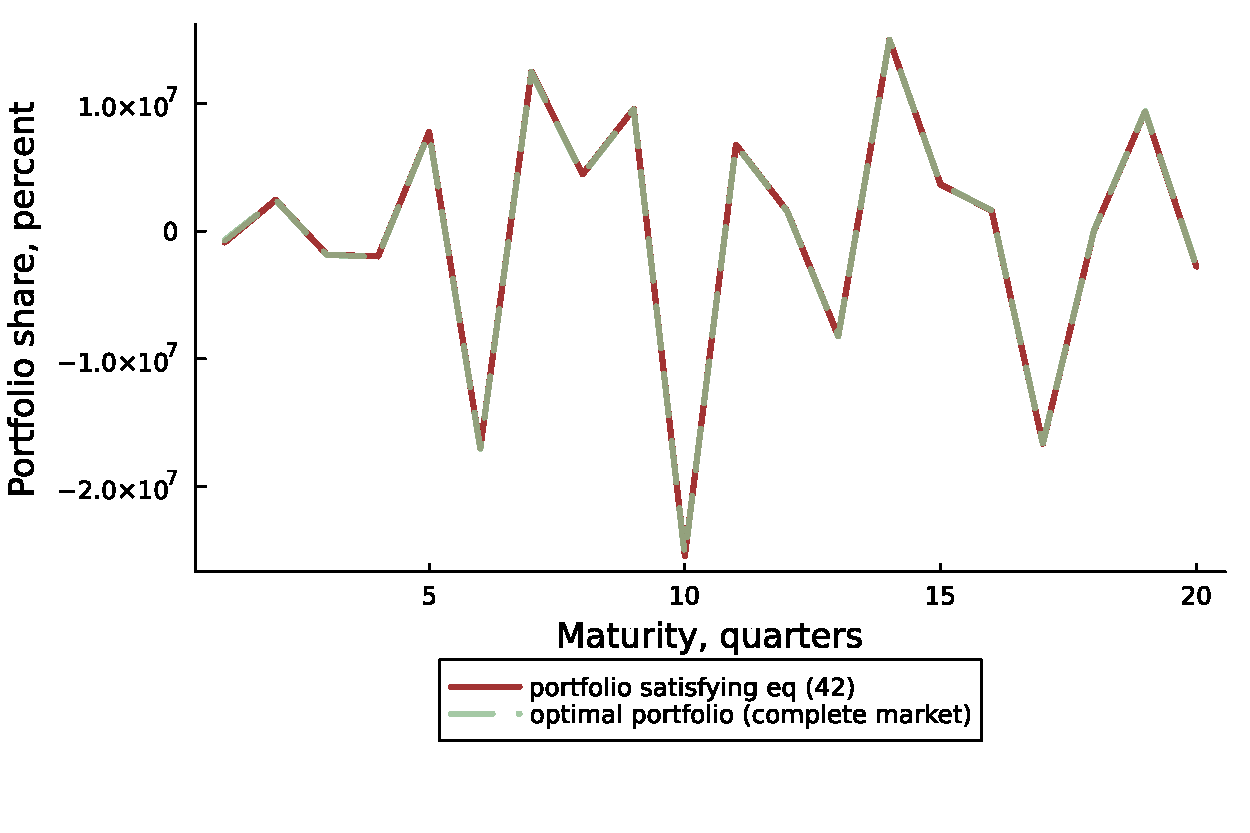
\includegraphics[scale=0.5]{figdata/body/ABN_BEGGS_20_states_bin_1_State_10}

\noindent\begin{minipage}[t]{1\columnwidth}%
{\scriptsize{}Notes: Government portfolio shares $\omega^{i}$ of
20 pure discount bonds of maturities $i\in\text{\ensuremath{\left\{ 1,\dots,20\right\} } }$
quarters. The green line is the portfolio implementing the complete
market allocation following \citet{AngeletosQJE2002}. The dark line
is the portfolio defined by problem (\ref{eq: tolerance}) taken for
the average state, that is $s=10$ in the ergodic distribution of
$G$. The tolerance is $\epsilon=10^{-8}$.}%
\end{minipage}{\scriptsize{}{}{}{}{}{}{}}{\scriptsize\par}
\end{figure}

What would our statistical summary approach to approximating an optimal
portfolio tell us for this economy? Returns on different bonds are
highly correlated in the neoclassical economy, which makes the matrix
of returns $\Sigma$ nearly singular. For that reason, we focus on
formula (\ref{eq: main result matrix form}), which does not require
inverting $\Sigma$. To make formula (\ref{eq: w* TFP}) operational,
we fix a tolerance level $\epsilon>0$ and let $s_{t}=s_{10}$, study
portfolios $\omega_{t}^{*}$ that satisfy 
\begin{equation}
\left\Vert \Sigma_{t}\omega_{t}^{*}-\left[\Sigma_{t}^{Q}s_{t}^{Q}+\Sigma_{t}^{G}s_{t}^{G}+\Sigma_{t}^{\Theta}s_{t}^{\Theta}\right]\mathtt{}\right\Vert \leq\epsilon,\label{eq: tolerance}
\end{equation}
where $\left\Vert \cdot\right\Vert $ is the $L^{1}$ norm. For sufficiently
small tolerance levels that we have studied, we found that a portfolio
that satisfies (\ref{eq: tolerance}) is very close to the theoretical
optimal portfolio computed above. The dashed line in Figure \ref{fig: Government-portfolio-shares_Angeletos_and_us}
presents this portfolio for $\epsilon=10^{-8}$. Thus, in the Angeletos
environment, ignoring income and price effects in deriving equation
(\ref{eq: w* TFP}) does not impair its ability to approximate an
optimal portfolio well.

Since our statistical formulas are reliable guides for constructing
an optimal portfolios in the neoclassical model, we can use them to
understand what drives differences between our prescribed optimal
government portfolio and the one that emerges from the standard growth
model. In Table \ref{tab:covariances abn-1-1}, we produce version
of Table \ref{tab:covariances} but now estimated from simulations
of a neoclassical growth model instead of U.S. data. We scale the
moments simulated from the neoclassical model by 100 for ease of comparison.
We find that simulations of the neoclassical model generate counterfactual
statistics for volatilities of bond prices and also for their co-movements
with macroeconomic aggregates. For instance, for long maturities the
variance of returns is 300 times smaller than their counterparts in
U.S. data. The covariances of returns with primary government surpluses
are only 10-20 times smaller, indicating much higher correlations.
Furthermore, returns and surpluses are positively correlated and of
opposite sign from those in U.S. data. 
\begin{table}[H]
\centering

\caption{{\small{}{}{}{}{}{}{}DATA vs NEOCLASSICAL MODEL\label{tab:covariances abn-1-1}}}
\medskip{}

\centering

\medskip{}
 %
\begin{tabular}[t]{>{\raggedright}p{0.75cm}>{\centering}p{2cm}>{\centering}p{3cm}>{\centering}p{2cm}>{\centering}p{2cm}}
\hline 
\raggedright{}{\tiny{}{}} & \multicolumn{2}{c}{{\small{}Neoclassical Model}} & \multicolumn{2}{c}{Data}\tabularnewline
\hline 
{\scriptsize{}Mat} & {\scriptsize{}100 x Var(r)} & \raggedright{}{\scriptsize{}100 x Cov( r, X/Y)} & {\scriptsize{}Var(r)} & \raggedright{}{\scriptsize{}Cov( r, X/Y)}\tabularnewline
\hline 
\raggedright{}{\scriptsize{}6m} & {\footnotesize{}0.02} & {\footnotesize{}0.29} & {\footnotesize{}0.09} & {\footnotesize{}-0.01}\tabularnewline
\raggedright{}{\scriptsize{}12m} & {\footnotesize{}0.12} & {\footnotesize{}0.83} & {\footnotesize{}0.49} & {\footnotesize{}-0.10}\tabularnewline
\raggedright{}{\scriptsize{}18m} & {\footnotesize{}0.30} & {\footnotesize{}1.30} & {\footnotesize{}1.10} & {\footnotesize{}-0.17}\tabularnewline
\raggedright{}{\scriptsize{}24m} & {\footnotesize{}0.54} & {\footnotesize{}1.80} & {\footnotesize{}1.80} & {\footnotesize{}-0.26}\tabularnewline
\raggedright{}{\scriptsize{}30m} & {\footnotesize{}0.82} & {\footnotesize{}2.20} & {\footnotesize{}2.80} & {\footnotesize{}-0.31}\tabularnewline
\raggedright{}{\scriptsize{}36m} & {\footnotesize{}1.10} & {\footnotesize{}2.50} & {\footnotesize{}3.60} & {\footnotesize{}-0.40}\tabularnewline
\raggedright{}{\scriptsize{}42m} & {\footnotesize{}1.40} & {\footnotesize{}2.90} & {\footnotesize{}4.40} & {\footnotesize{}-0.45}\tabularnewline
\raggedright{}{\scriptsize{}48m} & {\footnotesize{}1.70} & {\footnotesize{}3.20} & {\footnotesize{}5.40} & {\footnotesize{}-0.50}\tabularnewline
\raggedright{}{\scriptsize{}54m} & {\footnotesize{}2.00} & {\footnotesize{}3.40} & {\footnotesize{}6.10} & {\footnotesize{}-0.56}\tabularnewline
\raggedright{}{\scriptsize{}60m} & {\footnotesize{}2.30} & {\footnotesize{}3.70} & {\footnotesize{}7.80} & {\footnotesize{}-0.62}\tabularnewline
\raggedright{}{\scriptsize{}120m} & {\footnotesize{}3.60} & {\footnotesize{}4.60} & {\footnotesize{}10.00} & {\footnotesize{}-0.75	}\tabularnewline
\end{tabular} \medskip{}

{\scriptsize{}{}{}{}{}{}{}{}}%
\noindent\begin{minipage}[t]{1\columnwidth}%
{\footnotesize{}{}{}{}{}{}Notes: We simulate the neoclassical
model for 265 quarters that correspond to the sample period 1952-2017.
The values in the columns for the Neoclassical model are multiplied
by 100. Excess returns 6m, 12m, ... are the nominal excess returns
in Fama maturity portfolios corresponding to 6-12 months, 12-18 months,
... maturity bins, respectively. The values in the data column are
quarterly and in percentage points.}%
\end{minipage}{\scriptsize{}{}{}{}{}{}{}}{\scriptsize\par}
\end{table}


\subsection{Reconciling the neoclassical portfolio}

Since the matrix $\Sigma_{t}$ in the neoclassical setup is nearly
singular, other portfolios also approximately satisfy equation (\ref{eq: w* TFP})
and attain levels of welfare that are close to welfare attainable
by trading a complete set of Arrow securities. To ensure that our
results are not driven by lack of invertibility of $\Sigma_{t}$,
we consider a special case in which the underlying Markov state $s_{t}$
takes two values and the exogenous spending process $G_{t}$ is calibrated
to the same moments as above. The advantage of the two state setup
is that we can implement the complete market allocation with a one-period
bond and a consol that pays one unit of consumption in perpetuity.
In this case $\omega^{*}$ is a scalar and represents the share in
the consol.

First, we use the formula from \citet{AngeletosQJE2002}, and then
we implement formula (\ref{eq: w*}) using objects constructed from
the model-simulated economy. In this portfolio, it is optimal for
the government to issue debt of $7$ to $8$ times annual GDP in the
consol. This finding is consistent with findings from a similar exercise
in \citet{AngeletosQJE2002} and confirms that in the neoclassical
growth model, long maturity debt is an excellent hedge against primary
surplus risk. As before, from the lens of our formula, we can trace
the source of this large position to the values of the covariance
of returns and spending, and the volatility of the returns on the
consol. In the calibrated model, the ergodic averages of $cov_{t}\left(X_{t+1},r_{t+1}^{consol}\right)/var_{t}(r_{t+1}^{consol})=1.48$
and $var_{t}\left(r_{t+1}^{consol}\right)=\left(0.18\%\right)^{2}$
as compared to $-0.061$ and $(3.5\%)^{2}$ in the data\footnote{We approximate the return on the consol by constructing an weighted
average of the 11 CRSP portfolios.} implying an hedging spending risk component that is positive, large
and equals $7.82$ times GDP in line with shares obtain from using
the formula from \citet{AngeletosQJE2002}.

Our analysis calls for sources of variation in bond returns that are
orthogonal to fiscal risks. \citet{BEGS4_old} described extensions
of a neoclassical growth model with discount factor shocks in the
spirit of \citet{Albuquerque_etalJF2016} and shows that the model
can produce less extreme portfolios. We can modify the two state risk-free
bond and consol setup in a similar fashion to illustrate the main
insight of how introducing discount factor shocks can help realign
theoretical results with statistics summarized in Tables \ref{tab:covariances}
and thereby imply an optimal public portfolio closer to those prescribed
in Section \ref{sec: target portfolio}.

To that end, we introduce a state-dependent discount factor, $\delta(s^{t})\beta^{t}$
and calibrate $\delta(s^{t})$ so that its mean is one and we additionally
match the sign and the magnitude of the ratio $cov_{t}\left(X_{t+1},r_{t+1}^{consol}\right)/var_{t}(r_{t+1}^{consol})$
in the ergodic distribution to its data counterpart. The calibrated
model produces volatile returns with variance of quarterly returns
equal $\left(4\%\right)^{2}$ which is roughly in line with variance
of long bonds in the U.S. Applying either \citet{AngeletosQJE2002}
formula or our expression (\ref{eq: w* TFP}), we find that matching
these asset pricing moments lowers the consol share of total debt
by an order of magnitude to $70\%$ of GDP and the rest $30\%$ in
the risk-free bond. These holdings are much more similar to ones we
found in Section \ref{sec: target portfolio}. We conclude that neoclassical
settings that misrepresents the asset return movements are an inappropriate
tool for studying optimal public portfolios whose composition depend
critically on the properties of co-movements between returns and macroeconomic
variables.

\section{Concluding remarks\label{sec:Conclusion}}

We have studied determinants of optimal public portfolios in a broad
class of dynamic stochastic equilibrium models that encompass various
specifications of attitudes towards risk, heterogeneities among households,
limits on market participations, and sources of liquidity. We use
small noise expansions to summarize determinants of optimal public
portfolios in terms of a small number of statistics that are functions
only of asset prices and macroeconomic variables. For recent U.S.
data, we find that an optimal portfolio is simple, stable over time,
and has bond shares that decay approximately exponentially with bond
maturity. We show that differences between our paper's optimal public
portfolio and those prescribed by earlier neoclassical models come
from features of those earlier models that lead them to misrepresent
observed covariances of asset returns with macroeconomic aggregates.

This paper focuses exclusively on timing protocols in which a government
commits to a fiscal plan and cannot default. Natural next steps would
explore alternative timing protocols by proceeding along lines advocated
by \citet{ArellanoRamanarayananJPE2012}, \citet{AAHW2019}, \citet{BocolaDovisAER2019},
and others. %We plan  to take steps in
%those directions.
\section{Data Availability\label{sec:Data-Availability}}
Code replicating the tables and figures in this article can be found in \citet{delannoy2024_managingpublicportfolios} in the Harvard Dataverse,  \url{https://doi.org/10.7910/DVN/I4HZ3S}.



\pagebreak{}

\vspace{0in}

\bibliographystyle{econ_aer}
\bibliography{BEGS4_new}

\vspace{0in}

\end{document}
